% !TEX TS-program = lualatex
\documentclass[aspectratio=169,8pt]{beamer}

\newcommand{\DocID}{IFOG-VPROTO-SLIDE-001}
\newcommand{\DocVersion}{v4.0.1}
\newcommand{\DocDate}{2026-11-26}

% --- Fonts & Vietnamese UTF-8 Support (LuaLaTeX) ---
\usepackage{fontspec}
\setmainfont{Noto Sans}
\setsansfont{Noto Sans}
\setmonofont{DejaVu Sans Mono}[Scale=0.84]
\usefonttheme[onlymath]{serif}

% --- Academic Math, Tables, Graphics & Vector Drawing ---
\usepackage{amsmath,amssymb,mathtools}
\usepackage{booktabs,tabularx,array,colortbl}
\usepackage{graphicx}
\usepackage{xcolor}
\usepackage{tikz}
\usetikzlibrary{arrows.meta,positioning,fit,shapes.geometric,backgrounds,calc,decorations.pathreplacing}
\usepackage{pgfplots}
\pgfplotsset{compat=1.18}
\usepackage[american]{circuitikz}
\usepackage[most]{tcolorbox}

% --- Restrained Academic Color Palette (IEEE / SPIE / Doctoral Seminar) ---
\definecolor{AcadNavy}{HTML}{0F294A}
\definecolor{AcadNavyDark}{HTML}{091A30}
\definecolor{AcadSlate}{HTML}{2B5B84}
\definecolor{AcadTeal}{HTML}{0E6251}
\definecolor{AcadTealBg}{HTML}{EEF7F5}
\definecolor{AcadBg}{HTML}{F6F8FB}
\definecolor{AcadRule}{HTML}{C7D3E0}
\definecolor{AcadText}{HTML}{1A202C}
\definecolor{AcadMuted}{HTML}{52606D}
\definecolor{AcadCrimson}{HTML}{8B1E3F}
\definecolor{AcadAmber}{HTML}{9C6500}
\definecolor{AcadAmberBg}{HTML}{FDF9EE}

% --- Beamer Academic Theme Configuration ---
\usetheme{default}
\usecolortheme{default}
\setbeamertemplate{navigation symbols}{}
\setbeamercolor{normal text}{fg=AcadText,bg=white}
\setbeamercolor{structure}{fg=AcadNavy}
\setbeamercolor{frametitle}{fg=AcadNavy,bg=white}
\setbeamercolor{item}{fg=AcadSlate}
\setbeamercolor{subitem}{fg=AcadTeal}
\setbeamercolor{enumerate item}{fg=AcadNavy}
\setbeamercolor{section in head/foot}{fg=white,bg=AcadNavy}
\setbeamercolor{section in head/foot shaded}{fg=white!55!AcadNavy,bg=AcadNavy}

\setbeamersize{text margin left=0.55cm,text margin right=0.55cm}
\setbeamerfont{itemize/enumerate subbody}{size=\scriptsize}

% Subtle Top Academic Section Breadcrumb Bar
\setbeamertemplate{headline}{%
  \leavevmode%
  \begin{beamercolorbox}[wd=\paperwidth,ht=0.34cm,dp=0.10cm,leftskip=0.20cm,rightskip=0.20cm]{section in head/foot}%
    \tiny\insertsectionnavigationhorizontal{\dimexpr\paperwidth-0.40cm\relax}{}{\hfill}%
  \end{beamercolorbox}%
}

% Clean 2-Line Academic Frametitle (Zero Top Clipping)
\makeatletter
\setbeamertemplate{frametitle}{%
  \nointerlineskip%
  \begin{beamercolorbox}[wd=\paperwidth,sep=0pt,leftskip=0.55cm,rightskip=0.55cm]{frametitle}%
    \vspace{0.12cm}%
    \noindent\raisebox{-0.03cm}{\textcolor{AcadTeal}{\rule{3pt}{0.34cm}}}\hspace{0.15cm}%
    {\normalsize\bfseries\insertframetitle}\par
    \ifx\insertframesubtitle\@empty\else%
      \vspace{0.01cm}%
      \noindent\hspace{0.26cm}{\scriptsize\color{AcadMuted}\insertframesubtitle}\par
    \fi%
    \vspace{0.05cm}%
    \noindent\textcolor{AcadRule}{\rule{\dimexpr\paperwidth-1.10cm\relax}{0.45pt}}%
    \vspace{0.04cm}%
  \end{beamercolorbox}%
}
\makeatother

% Crisp Academic Footline
\setbeamertemplate{footline}{%
  \vbox{%
    \hbox{\textcolor{AcadRule}{\rule{\paperwidth}{0.4pt}}}%
    \nointerlineskip%
    \hbox{%
      \begin{beamercolorbox}[wd=.44\paperwidth,ht=0.30cm,dp=0.11cm,leftskip=0.55cm]{footline}%
        \tiny\color{AcadMuted}\textbf{ifog-vproto \DocVersion} \enspace|\enspace \texttt{IFOG-SIM-SPEC-007}%
      \end{beamercolorbox}%
      \begin{beamercolorbox}[wd=.36\paperwidth,ht=0.30cm,dp=0.11cm,center]{footline}%
        \tiny\color{AcadMuted}\textit{\insertsectionhead}%
      \end{beamercolorbox}%
      \begin{beamercolorbox}[wd=.20\paperwidth,ht=0.30cm,dp=0.11cm,rightskip=0.55cm]{footline}%
        \hfill\tiny\color{AcadNavy}\textbf{\insertframenumber\ / \inserttotalframenumber}%
      \end{beamercolorbox}%
    }%
  }%
}

% --- Academic Styled Boxes (Hairline Borders, Compact Academic Typography) ---
\newtcolorbox{eqbox}[1][]{%
  enhanced,
  colback=AcadBg,
  colframe=AcadRule,
  borderline west={2.2pt}{0pt}{AcadNavy},
  arc=1.5pt,
  boxrule=0.4pt,
  left=5pt,right=5pt,top=2.5pt,bottom=2.5pt,
  toptitle=1.5pt,bottomtitle=1.5pt,
  fontupper=\scriptsize,
  before upper={\raggedright\setlength{\abovedisplayskip}{1.5pt}\setlength{\belowdisplayskip}{1.5pt}\setlength{\abovedisplayshortskip}{1pt}\setlength{\belowdisplayshortskip}{1pt}\setlength{\jot}{1.5pt}},
  fonttitle=\bfseries\scriptsize\color{AcadNavy},
  coltitle=AcadNavy,
  colbacktitle=AcadNavy!8!white,
  title={#1}
}

\newtcolorbox{remarkbox}[1][]{%
  enhanced,
  colback=AcadTealBg,
  colframe=AcadTeal!35,
  borderline west={2.2pt}{0pt}{AcadTeal},
  arc=1.5pt,
  boxrule=0.4pt,
  left=5pt,right=5pt,top=2.5pt,bottom=2.5pt,
  toptitle=1.5pt,bottomtitle=1.5pt,
  fontupper=\scriptsize,
  before upper={\raggedright\setlength{\abovedisplayskip}{1.5pt}\setlength{\belowdisplayskip}{1.5pt}},
  fonttitle=\bfseries\scriptsize\color{AcadTeal},
  coltitle=AcadTeal,
  colbacktitle=AcadTeal!12!white,
  title={#1}
}

\newtcolorbox{notebox}[1][]{%
  enhanced,
  colback=AcadAmberBg,
  colframe=AcadAmber!40,
  borderline west={2.2pt}{0pt}{AcadAmber},
  arc=1.5pt,
  boxrule=0.4pt,
  left=5pt,right=5pt,top=2.5pt,bottom=2.5pt,
  toptitle=1.5pt,bottomtitle=1.5pt,
  fontupper=\scriptsize,
  before upper={\raggedright\setlength{\abovedisplayskip}{1.5pt}\setlength{\belowdisplayskip}{1.5pt}},
  fonttitle=\bfseries\scriptsize\color{AcadAmber},
  coltitle=AcadAmber,
  colbacktitle=AcadAmber!12!white,
  title={#1}
}

\newcommand{\eqtag}[1]{\hfill{\tiny\color{AcadSlate}\texttt{(#1)}}}

\begin{document}

% ==============================================================================
% SLIDE 1: ACADEMIC TITLE SLIDE
% ==============================================================================
\begin{frame}[plain]
\begin{tikzpicture}[remember picture,overlay]
  \fill[AcadNavyDark] (current page.south west) rectangle (current page.north east);
  \fill[AcadNavy] (current page.north west) rectangle ([yshift=-5.45cm]current page.north east);
  \fill[AcadTeal] ([yshift=-5.45cm]current page.north west) rectangle ([yshift=-5.62cm]current page.north east);
  % Clean subtle geometric Sagnac coil rings on upper right (no text collision)
  \begin{scope}[shift={([xshift=-2.15cm,yshift=-2.65cm]current page.north east)}]
    \foreach \r/\op in {2.10/0.06, 1.80/0.08, 1.50/0.11, 1.20/0.14} {
      \draw[white,opacity=\op,line width=0.85pt] (0,0) circle (\r cm);
    }
    \draw[AcadTeal!70!white,opacity=0.30,line width=1.0pt,-{Stealth[length=2mm]}] (60:1.50cm) arc (60:-30:1.50cm);
    \draw[AcadAmber!75!white,opacity=0.30,line width=1.0pt,-{Stealth[length=2mm]}] (120:1.20cm) arc (120:210:1.20cm);
  \end{scope}
\end{tikzpicture}

\vspace{0.55cm}
{\scriptsize\color{AcadTealBg}\textbf{CHUYÊN ĐỀ KHOA HỌC \& KIẾN TRÚC BẢN SAO SỐ QUANG–ĐIỆN TỬ} \enspace|\enspace \texttt{\DocID}}\\[0.32cm]
{\LARGE\bfseries\color{white} Closed-Loop IFOG Multi-Scale Virtual Prototype}\\[0.20cm]
{\normalsize\color{AcadTealBg} Phương pháp luận, Mô hình Toán học và Quy trình Mô phỏng Con quay Sợi quang Vòng kín}\\[0.28cm]
{\footnotesize\color{white!82!gray} Đa thang thời gian 3 Tầng \enspace$\bullet$\enspace Điều biến 6 Trạng thái Đối xứng \enspace$\bullet$\enspace Chuẩn FMI 3.0 FMU \enspace$\bullet$\enspace Hiệu chuẩn Ngược $<5\%$}

\vspace{1.35cm}
\begin{columns}[T]
  \begin{column}{0.235\textwidth}
    \begin{tcolorbox}[colback=AcadNavy!90!black,colframe=AcadTeal!80,arc=2pt,boxrule=0.5pt,left=6pt,right=6pt,top=4pt,bottom=4pt]
      {\large\bfseries\color{white} $10^{11}\times$}\\[-1pt]
      {\scriptsize\color{AcadTealBg} Dải thang thời gian\\$153\text{ ns} \leftrightarrow 10\text{ giờ}$}
    \end{tcolorbox}
  \end{column}
  \begin{column}{0.235\textwidth}
    \begin{tcolorbox}[colback=AcadNavy!90!black,colframe=AcadTeal!80,arc=2pt,boxrule=0.5pt,left=6pt,right=6pt,top=4pt,bottom=4pt]
      {\large\bfseries\color{white} 53 / 53}\\[-1pt]
      {\scriptsize\color{AcadTealBg} Công thức truy vết\\(\texttt{EQ-01}..\texttt{EQ-53})}
    \end{tcolorbox}
  \end{column}
  \begin{column}{0.235\textwidth}
    \begin{tcolorbox}[colback=AcadNavy!90!black,colframe=AcadTeal!80,arc=2pt,boxrule=0.5pt,left=6pt,right=6pt,top=4pt,bottom=4pt]
      {\large\bfseries\color{white} 23 / 23}\\[-1pt]
      {\scriptsize\color{AcadTealBg} Cổng \& Kịch bản thật\\(\texttt{100\%} C++/Py cov)}
    \end{tcolorbox}
  \end{column}
  \begin{column}{0.235\textwidth}
    \begin{tcolorbox}[colback=AcadNavy!90!black,colframe=AcadTeal!80,arc=2pt,boxrule=0.5pt,left=6pt,right=6pt,top=4pt,bottom=4pt]
      {\large\bfseries\color{white} $< 1\%$}\\[-1pt]
      {\scriptsize\color{AcadTealBg} Sai số dự báo sau\\Hiệu chuẩn ngược}
    \end{tcolorbox}
  \end{column}
\end{columns}

\vspace{0.55cm}
{\scriptsize\color{white!75!gray}
\textbf{Nền tảng \& Đặc tả:} \texttt{ifog-vproto \DocVersion} (\texttt{IFOG-SIM-SPEC-007} v7.0; tương thích ngược \texttt{SPEC-006/005/004}) \hfill \textbf{Ngày:} \DocDate\\
\textbf{Chuẩn mực học thuật:} IEEE Std 952-2020 \enspace$\bullet$\enspace IEEE Std 1666.1-2016 (SystemC-AMS) \enspace$\bullet$\enspace FMI 3.0.2 \enspace$\bullet$\enspace Lefèvre (3rd Ed.)
}
\end{frame}

% ==============================================================================
% SECTION I: TỔNG QUAN & CƠ SỞ VẬT LÝ
% ==============================================================================
\section{I. Tổng quan}

% SLIDE 2: ĐẶT VẤN ĐỀ & NỘI DUNG TRÌNH BÀY
\begin{frame}{Đặt vấn đề Khoa học \& Cấu trúc Báo cáo}{Thách thức mô phỏng đa vật lý – đa thang thời gian của IFOG vòng kín}
\begin{columns}[T]
  \begin{column}{0.53\textwidth}
    \begin{eqbox}[1. Bài toán Khoa học Cốt lõi]
      \begin{itemize}\setlength\itemsep{3.5pt}
        \item \textbf{Độ cứng thang thời gian 11 bậc độ lớn:} Quá độ mạch TIA, cộng hưởng điện–âm học MIOC và gai reset $2\pi$ diễn ra ở thang $\Delta t \approx 153\text{--}306\text{ ns}$ ($f_s \approx 3.3\text{--}6.5\text{ MHz}$), trong khi đánh giá trôi Bias Instability \& Rate Random Walk (IEEE Std 952) đòi hỏi chuỗi đo $10\text{ giờ}$ ($3.6\times 10^4\text{ s}$).
        \item \textbf{Khoảng cách mô hình datasheet so với phần cứng ($>40\%$):} Các hiệu ứng ký sinh phi tuyến ghép nối chéo — \emph{Deadband}, \emph{Bunny Ears}, rò nhiễu $1/f$ qua bậc 3 TIA, xuyên nhiễu điện dung $C_{\text{xtalk}}\dot{V}$, ứng suất đàn hồi–quang và phản xạ ngược Rayleigh/facet — chi phối sai số thực tế của con quay cấp dẫn đường.
        \item \textbf{Yêu cầu bài toán ngược (Inverse Problem):} Cần tự động ước lượng các tham số ký sinh không đo trực tiếp được từ dữ liệu phòng thí nghiệm (AVAR tĩnh, ramp tốc độ chậm, buồng nhiệt) kèm khoảng tin cậy thống kê $95\%$.
      \end{itemize}
    \end{eqbox}
  \end{column}
  \begin{column}{0.45\textwidth}
    \begin{remarkbox}[2. Cấu trúc Nội dung (6 Phần)]
      \begin{enumerate}\setlength\itemsep{3pt}
        \item \textbf{Cơ sở Vật lý IFOG:} Sơ đồ giao thoa kế Sagnac vòng kín và các nguồn sai số không thuận nghịch.
        \item \textbf{Kiến trúc 3 Tầng \& Quy trình:} Tách miền thời gian $10^{11}\times$, quy trình 6 bước và hợp đồng an toàn đóng.
        \item \textbf{Tầng 1 (Quang–Nhiệt Offline):} Ma trận Jones phân lát phổ, quấn Quadrupole/Octupole, Shupe, ứng suất và LUT v2.
        \item \textbf{Tầng 2 (SystemC-AMS \& DSP):} MIOC bậc 2, mạch TIA+$C_{\text{xtalk}}$, Blanking, DSP 6-State đối xứng, IMU 3 trục và BIT.
        \item \textbf{FMI 3.0 \& Tầng 3:} Đóng gói FMU chuẩn công nghiệp, AVAR 5 vùng chế độ kép và Hiệu chuẩn ngược 3 giai đoạn.
        \item \textbf{Thực nghiệm \& Kiểm chứng:} Phân tích định lượng 23 kịch bản, độ phủ $100\%$, CI/CD chọn lọc theo \texttt{git diff}.
      \end{enumerate}
    \end{remarkbox}
  \end{column}
\end{columns}

\vspace{0.14cm}
\begin{notebox}[Tính nhất quán giữa Lý thuyết và Thực thi (Spec-to-Code Traceability)]
  Mọi phương trình ký hiệu \texttt{(EQ-01)}..\texttt{(EQ-53)} trong bài trình bày tương ứng 1-đối-1 với đặc tả toán học \texttt{IFOG-SIM-SPEC-004..007} và được kiểm chứng tự động bằng 53 bộ kiểm thử công thức độc lập trên lõi C++17 / Python 3.12.
\end{notebox}
\end{frame}

% SLIDE 3: NGUYÊN LÝ VẬT LÝ IFOG VÒNG KÍN (TIKZ FIG 1)
\begin{frame}{Nguyên lý Vật lý Con quay Sợi quang Vòng kín (Closed-Loop IFOG)}{Cấu trúc giao thoa kế Sagnac tối thiểu (Minimum Configuration) \& vòng hồi tiếp triệt pha}
\begin{center}
\begin{tikzpicture}[
    scale=0.78, transform shape,
    opt/.style={rectangle,rounded corners=2pt,draw=AcadNavy,fill=AcadBg,thick,align=center,font=\scriptsize,minimum height=0.80cm,inner sep=3.5pt},
    elec/.style={rectangle,rounded corners=2pt,draw=AcadTeal,fill=AcadTealBg,thick,align=center,font=\scriptsize,minimum height=0.80cm,inner sep=3.5pt},
    dsp/.style={rectangle,rounded corners=2pt,draw=AcadCrimson,fill=AcadCrimson!7,thick,align=center,font=\scriptsize,minimum height=0.80cm,inner sep=3.5pt},
    oarr/.style={-{Stealth[length=2mm]},thick,AcadNavy},
    earr/.style={-{Stealth[length=2mm]},thick,AcadTeal},
    farr/.style={-{Stealth[length=2mm]},thick,AcadCrimson}
]
  % Optical top path
  \node[opt,minimum width=1.85cm] (sld) {\textbf{Nguồn SLD}\\$\bar{\lambda}=1550\text{ nm}$\\$L_c\approx 60\ \mu\text{m}$};
  \node[opt,right=0.65cm of sld,minimum width=1.65cm] (cpl) {\textbf{Bộ tách 3 dB}\\(Coupler)\\Tách / Thu tia};
  \node[opt,right=0.75cm of cpl,minimum width=2.45cm] (mioc) {\textbf{Chip MIOC ($\text{LiNbO}_3$)}\\Phân cực + Y-junction\\Bộ điều biến pha $\phi_{\text{MIOC}}(t)$};

  % Fiber Coil (Sagnac Loop) on right — clean non-overlapping labels
  \begin{scope}[shift={($(mioc.east)+(2.55,0)$)}]
    \draw[AcadNavy,very thick,fill=AcadBg] (0,0) circle (1.08cm);
    \draw[AcadSlate,thick] (0,0) circle (0.93cm);
    \draw[AcadSlate,thin] (0,0) circle (0.79cm);
    \node[align=center,font=\scriptsize,AcadNavy] at (0,0) {\textbf{Cuộn sợi PM}\\$L,\,D,\,N_{\text{turns}}$\\$\tau = n_{\text{eff}}L/c$};
    \draw[AcadTeal,thick,-{Stealth[length=1.8mm]}] (128:1.24cm) arc (128:52:1.24cm) node[midway,above,font=\tiny,AcadTeal]{CW};
    \draw[AcadCrimson,thick,-{Stealth[length=1.8mm]}] (-52:1.24cm) arc (-52:-128:1.24cm) node[midway,below,font=\tiny,AcadCrimson]{CCW};
    % External rotation indicator on right of coil
    \draw[AcadAmber,thick,-{Stealth[length=1.8mm]}] (-32:1.30cm) arc (-32:32:1.30cm) node[midway,right,font=\scriptsize\bfseries,AcadAmber]{$\Omega_{\text{in}}(t)$};
    \coordinate (coilTop) at (155:1.08cm);
    \coordinate (coilBot) at (-155:1.08cm);
  \end{scope}

  % Optical connections
  \draw[oarr] (sld) -- (cpl);
  \draw[oarr,<->] (cpl) -- node[above,font=\tiny]{$P_0$} (mioc);
  \draw[oarr] ([yshift=0.22cm]mioc.east) -- (coilTop);
  \draw[oarr] (coilBot) -- ([yshift=-0.22cm]mioc.east);

  % Electronic & DSP bottom path
  \node[elec,below=1.10cm of cpl,minimum width=2.05cm] (pd) {\textbf{Photodiode + TIA}\\$\mathcal{R}P_{\text{det}} \to V_{\text{TIA}}(t)$\\6 nhiễu + $G_2,G_3$};
  \node[elec,right=0.60cm of pd,minimum width=1.95cm] (adc) {\textbf{ADC + Blanking}\\Bỏ mẫu gai $[k_s,k_e]$\\$N_{\text{ADC}}$ bit + Jitter};
  \node[dsp,right=0.60cm of adc,minimum width=2.70cm] (dsp) {\textbf{FPGA DSP (6-State)}\\Vòng 1: Khóa Sagnac ($\Delta\phi_{\text{step}}$)\\Vòng 2: Khóa $V_\pi$ ($\hat{g}_{\text{DAC}}$)};
  \node[elec,right=0.60cm of dsp,minimum width=2.05cm] (dac) {\textbf{DAC + Driver}\\Bậc thang + Reset $2\pi$\\$V_{\text{drv}}(t)$ ($N_{\text{DAC}}$ bit)};

  % Electronic connections
  \draw[oarr] (cpl.south) -- node[right,font=\tiny]{$P_{\text{det}}(t)$} (pd.north);
  \draw[earr] (pd) -- (adc);
  \draw[earr] (adc) -- node[above,font=\tiny]{$y[n]$} (dsp);
  \draw[farr] (dsp) -- node[above,font=\tiny]{$\phi_{\text{cmd}}$} (dac);
  \draw[farr] (dac.north) -- ++(0,0.34) -| node[pos=0.73,left,font=\tiny,AcadCrimson]{$V_{\text{drv}}(t)$} (mioc.south);
  % Digital output cleanly under DSP (above crosstalk bus)
  \draw[farr] (dsp.south) -- ++(0,-0.32) node[below,font=\tiny\bfseries,AcadCrimson,fill=white,inner sep=1pt]{$\Omega_{\text{out}}[n] = \Delta\phi_{\text{step}}[n] / \mathrm{SF}_{\text{CL}}$};
  % Crosstalk parasitic bus routed cleanly below digital output
  \draw[AcadAmber,dashed,thick,-{Stealth[length=1.8mm]}] (dac.south) -- ++(0,-0.78) -| node[pos=0.28,below,font=\tiny,AcadAmber]{Xuyên nhiễu PCB: $i_{\text{xtalk}} = G_{\text{xtalk}}V_{\text{drv}} + C_{\text{xtalk}}\dot{V}_{\text{drv}}$} (pd.south);
\end{tikzpicture}
\end{center}

\vspace{0.08cm}
\begin{columns}[T]
  \begin{column}{0.49\textwidth}
    \begin{eqbox}[Cơ chế Triệt pha (Nulling) Vòng kín]
      Khi cuộn sợi quay với vận tốc góc $\Omega_{\text{in}}$, hai tia CW/CCW lệch pha Sagnac $\Delta\phi_S = K_{\text{opt}}\Omega_{\text{in}}$. Bộ DSP bơm bậc thang pha $\Delta\phi_{\text{step}}$ (kèm điều biến đối xứng $\psi_s$ và reset $2\pi$) sao cho $\Delta\phi_{\text{NR}} + \Delta\phi_{\text{fb}} = 0$ tại mọi chu kỳ $\tau$.
    \end{eqbox}
  \end{column}
  \begin{column}{0.49\textwidth}
    \begin{remarkbox}[Ưu điểm Học thuật của Kiến trúc Vòng kín]
      Điểm làm việc luôn giữ cố định tại vị trí nhạy cực đại của hàm $\cos(\cdot)$, giúp hệ số tỷ lệ $\mathrm{SF}_{\text{CL}}$ tuyến tính trong dải rộng ($\pm 700^\circ/\text{s}$), độc lập với biến thiên công suất nguồn $P_0$ và độ tương phản vân $V$.
    \end{remarkbox}
  \end{column}
\end{columns}
\end{frame}

% ==============================================================================
% SECTION II: KIẾN TRÚC & QUY TRÌNH
% ==============================================================================
\section{II. Kiến trúc \& Quy trình}

% SLIDE 4: KIẾN TRÚC 3 TẦNG + THANG THỜI GIAN 11 BẬC (TIKZ FIG 2)
\begin{frame}{Phương pháp Mô phỏng Đa thang đo: Kiến trúc 3 Tầng + FMI 3.0}{Phân tách miền vật lý trên 11 bậc thang thời gian ($153\text{ ns} \to 10\text{ giờ}$)}
\begin{center}
% Multi-scale logarithmic time axis
\begin{tikzpicture}[scale=0.92, transform shape]
  % Top logarithmic axis
  \draw[-{Stealth[length=2.2mm]},thick,AcadSlate] (0,0) -- (14.4,0);
  \foreach \x/\lbl in {0.4/$10^{-7}\text{ s}$, 2.6/$10^{-5}\text{ s}$, 4.8/$10^{-3}\text{ s}$, 7.0/$10^{-1}\text{ s}$, 9.2/$10^{1}\text{ s}$, 11.4/$10^{3}\text{ s}$, 13.6/$10^{4}\text{ s}$} {
    \draw[AcadSlate,thick] (\x,-0.08) -- (\x,0.08);
    \node[below,font=\tiny,AcadMuted] at (\x,-0.08) {\lbl};
  }
  \fill[AcadTeal,opacity=0.22] (0.5,0.12) rectangle (8.7,0.44);
  \node[font=\tiny\bfseries,AcadTeal] at (4.6,0.28) {Tầng 2 (SystemC-AMS Fast-Scale): $\Delta t = 153\text{ ns} \dots 60\text{ s}$};
  \fill[AcadAmber,opacity=0.35] (7.0,0.12) rectangle (8.7,0.44);
  \node[above,font=\tiny\bfseries,AcadAmber] at (7.85,0.44) {Vùng chồng $[0.1, 5]\text{ s}$ ($<5\%$)};
  \fill[AcadNavy,opacity=0.16] (7.0,0.12) rectangle (13.8,0.44);
  \node[font=\tiny\bfseries,AcadNavy] at (11.25,0.28) {Tầng 3 (Slow-Scale AVAR): $10\text{ ms} \dots 10\text{ h}$};
\end{tikzpicture}

\vspace{0.10cm}
\begin{tikzpicture}[
    scale=0.87, transform shape,
    box/.style={rectangle,rounded corners=2.5pt,draw=AcadNavy,fill=AcadBg,thick,align=center,font=\scriptsize,minimum width=3.55cm,minimum height=1.22cm,inner sep=3.5pt},
    t2box/.style={rectangle,rounded corners=2.5pt,draw=AcadTeal,fill=AcadTealBg,thick,align=center,font=\scriptsize,minimum width=4.05cm,minimum height=1.22cm,inner sep=3.5pt},
    fmubox/.style={rectangle,rounded corners=2.5pt,draw=AcadAmber,fill=AcadAmberBg,thick,align=center,font=\scriptsize,minimum width=4.05cm,minimum height=0.98cm,inner sep=3.5pt},
    arr/.style={-{Stealth[length=2mm]},thick,AcadNavy},
    tarr/.style={-{Stealth[length=2mm]},thick,AcadTeal}
]
  \node[box] (t1) {\textbf{TẦNG 1: Offline Solvers}\\{\tiny Python 3.12 / NumPy / SciPy}\\Jones phân cực + Cuộn dây Quad/Oct\\Shupe + Ứng suất + $K_{\text{opt}}(t)$};
  \node[t2box,right=1.75cm of t1] (t2) {\textbf{TẦNG 2: Fast-Scale Core}\\{\tiny C++17 \texttt{-O3 -fPIC} / SystemC-AMS}\\Quang + MIOC bậc 2 + TIA + $C_{\text{xtalk}}$\\ADC/DAC + DSP 2/4/6-State + BIT};
  \node[box,right=1.75cm of t2] (t3) {\textbf{TẦNG 3: Long-Term \& Calibration}\\{\tiny Python + FMPy + SciPy TRF}\\Ma trận $\mathbf{K}$, AVAR 5 vùng 10 giờ\\23 kịch bản + \texttt{InverseCalibrator}};

  \node[box,fill=AcadNavy!8,below=0.58cm of t1,minimum height=0.98cm] (cfg) {\textbf{Cấu hình \& Ràng buộc}\\{\tiny \texttt{schema\_v6.json} (Rule 11)}\\Ổn định Jury + Seed tất định};
  \node[fmubox,below=0.58cm of t2] (fmu) {\textbf{FMI 3.0 Co-Sim FMU (\texttt{ifog\_core.fmu})}\\{\tiny 75 hàm C-API | 22 biến SI (\texttt{VR 0..21})}\\Tương đương \texttt{0.00e+00 rad/s}};
  \node[box,draw=AcadTeal,fill=AcadTeal!8,below=0.58cm of t3,minimum height=0.98cm] (viz) {\textbf{Phân tích \& Xuất Báo cáo (\texttt{viz/})}\\23 hình 300-DPI + \texttt{report.md}\\HTML (KaTeX/Plotly) + PDF};

  \draw[arr] (cfg) -- (t1);
  \draw[arr] (cfg.east) -- ++(0.45,0) |- ([yshift=-0.34cm]t2.west);
  \draw[arr] (t1) -- node[above,font=\tiny]{\texttt{phys\_params.json}} node[below,font=\tiny]{\texttt{shupe\_lut.bin} v2} (t2);
  \draw[tarr] (t2) -- node[above,font=\tiny]{\texttt{sim\_out.bin} (32 B)} node[below,font=\tiny]{\texttt{micro/dsp} (64 B)} (t3);
  \draw[tarr,<->] (t2) -- (fmu);
  \draw[arr] (fmu.east) -- ++(0.60,0) |- ([yshift=-0.34cm]t3.west);
  \draw[tarr] (t3) -- (viz);
\end{tikzpicture}
\end{center}

\vspace{0.06cm}
\scriptsize
\renewcommand{\arraystretch}{1.06}
\begin{tabularx}{\textwidth}{@{}p{2.2cm} p{2.5cm} p{2.7cm} >{\raggedright\arraybackslash}X@{}}
\toprule
\textbf{Thành phần} & \textbf{Động cơ tính toán} & \textbf{Bước thời gian} & \textbf{Vai trò vật lý \& Chuẩn đầu ra} \\
\midrule
\textbf{Tier 1} & Python / SciPy & Tĩnh \& Nhiệt $0..10\text{ h}$ & Giải quang phân cực, 2D nhiệt CN/FEM $\to$ \texttt{phys\_params.json}, \texttt{shupe\_lut.bin} v2 (56 B) \\
\textbf{Tier 2} & C++17 / SystemC-AMS & $\Delta t = \tau/K \approx 153\text{ ns}$ & Mô phỏng vòng kín chuẩn bit tốc độ cao ($\approx 1.1\text{ s}$/s thực), ghi log 32 B / 64 B \\
\textbf{FMI 3.0 FMU} & \texttt{ifog\_core.so} & Bước $H \ge 1\text{ ms}$ (ZOH) & Hộp đen đồng mô phỏng Simulink/FMPy; mở 7 tham số ký sinh chỉnh nóng lúc chạy \\
\textbf{Tier 3} & Python / Multiprocess & $\Delta t_{\text{slow}}=10\text{ ms}$, $10\text{ h}$ & Ghép AVAR 5 vùng IEEE 952 ($<5\%$), 23 kịch bản, hiệu chuẩn ngược \texttt{calibrated\_params.json} \\
\bottomrule
\end{tabularx}
\end{frame}

% SLIDE 5: QUY TRÌNH MÔ PHỎNG KHOA HỌC ĐẦU–CUỐI (TIKZ FIG 3)
\begin{frame}{Quy trình Mô phỏng Khoa học Đầu–Cuối (End-to-End Methodology)}{Chuỗi thực thi 6 bước khép kín đảm bảo tính lặp lại và kiểm soát sai số toán học}
\begin{center}
\begin{tikzpicture}[
    scale=0.88, transform shape,
    wfstep/.style={rectangle,rounded corners=2.5pt,draw=AcadNavy,fill=AcadBg,thick,align=center,font=\scriptsize,minimum width=2.25cm,minimum height=1.85cm,inner sep=3.5pt},
    badge/.style={circle,fill=AcadNavy,text=white,font=\tiny\bfseries,inner sep=1.8pt},
    arr/.style={-{Stealth[length=2mm]},thick,AcadTeal}
]
  \node[wfstep] (s1) {\textbf{Nạp \& Kiểm tra}\\JSON \texttt{schema\_v6}\\Rule 11 Fail-Closed:\\$0<K_{\text{tot},1}<1$\\$K_{\text{tot},2}\le 0.1K_{\text{tot},1}$};
  \node[wfstep,right=0.42cm of s1] (s2) {\textbf{Giải Tầng 1}\\Jones $N_{\text{spec}}$ lát\\Quấn Quad/Oct\\Nhiệt CN / FEM\\$\to$ LUT v2 (6 kênh)};
  \node[wfstep,right=0.42cm of s2,draw=AcadTeal,fill=AcadTealBg] (s3) {\textbf{Chạy Tầng 2}\\SystemC-AMS \texttt{-O3}\\Single / IMU 3 trục\\hoặc FMI 3.0 FMU\\Ghi nhị phân 32/64B};
  \node[wfstep,right=0.42cm of s3] (s4) {\textbf{Phân tích Tầng 3}\\Quét Deadband\\FFT 100 Hz ($\mathbf{K}$)\\AVAR 5 vùng 10h\\Chống đếm trùng BI};
  \node[wfstep,right=0.42cm of s4] (s5) {\textbf{Hiệu chuẩn Ngược}\\Tối ưu TRF 3 bước\\AVAR+Ramp+Nhiệt\\10 tham số ẩn\\+ 95\% CI JSON};
  \node[wfstep,right=0.42cm of s5,draw=AcadSlate,fill=AcadNavy!7] (s6) {\textbf{Kiểm chứng \& BC}\\53 Formula Tests\\23 ảnh 300-DPI\\ \texttt{report.md/.html}\\Explorer HTML};

  \foreach \i/\nd in {1/s1, 2/s2, 3/s3, 4/s4, 5/s5, 6/s6} {
    \node[badge] at (\nd.north west) {\i};
  }
  \draw[arr] (s1) -- (s2);
  \draw[arr] (s2) -- (s3);
  \draw[arr] (s3) -- (s4);
  \draw[arr] (s4) -- (s5);
  \draw[arr] (s5) -- (s6);

  % Feedback validation loop
  \draw[AcadCrimson,dashed,thick,-{Stealth[length=2mm]}] (s5.south) -- ++(0,-0.42) -| node[pos=0.25,below,font=\tiny\bfseries,AcadCrimson]{Vòng kiểm tra chéo (Cross-Validation) trên lõi C++ thật: sai số dự báo $<5\%$ (đạt $0.034\%$)} (s3.south);
\end{tikzpicture}
\end{center}

\vspace{0.18cm}
\begin{columns}[T]
  \begin{column}{0.49\textwidth}
    \begin{eqbox}[Cơ chế Thực thi Linh hoạt qua CLI (31 Chế độ)]
      \begin{itemize}\setlength\itemsep{2.5pt}
        \item \textbf{Mô phỏng đơn lẻ theo bài toán:} \texttt{./scripts/run\_sim.sh --mode <mode>} (ví dụ \texttt{td\_blanking}, \texttt{dyn\_bode\_sweep}, \texttt{dyn\_sine\_electro\_optic}, \texttt{eng\_imu\_3axis}, \texttt{fmi\_gate}, \texttt{spec007\_calibration}).
        \item \textbf{Mô phỏng theo nhóm chuyên đề:} \texttt{full} (Gates 1--4), \texttt{td\_all}, \texttt{eng\_all}, \texttt{dyn\_all}, \texttt{spec007\_all}.
        \item \textbf{Chạy trọn bộ 23/23 kịch bản chuẩn:} \texttt{./scripts/run\_all\_scenarios.sh} tự động sinh toàn bộ đồ thị 300-DPI, \texttt{report.md}, \texttt{report.html} và \texttt{index.html}.
      \end{itemize}
    \end{eqbox}
  \end{column}
  \begin{column}{0.49\textwidth}
    \begin{remarkbox}[Cơ sở Học thuật LTF/Lefèvre \& Hợp đồng Tin cậy]
      \begin{itemize}\setlength\itemsep{2.0pt}
        \item \textbf{Tham chiếu chuẩn mực LTF (IEEE 1666.1) \& Lefèvre:} Mô phỏng tương tự dùng \textbf{Hàm truyền Tuyến tính LTF} (\texttt{sca\_ltf\_nd} trong SystemC-AMS TDF, kết hợp giải tích ma trận mũ ZOH cho hệ cứng $\omega_0\Delta t>0.2$) ghép nối chuẩn bit với DSP vòng kín theo Lefèvre (3rd Ed.) \& IEEE Std 952-2020.
        \item \textbf{Tất định (Rule 10) \& An toàn đóng (Rule 11):} Hạt giống tường minh (\texttt{seed}); từ chối chạy ngay nếu vi phạm ổn định Jury hoặc lệch kích thước struct nhị phân.
        \item \textbf{Độ chính xác IEEE-754 64-bit:} Bảo toàn gói pha modulo-$2\pi$ dưới $10^{-15}\text{ rad}$ qua hàng tỷ chu kỳ $\tau$.
      \end{itemize}
    \end{remarkbox}
  \end{column}
\end{columns}
\end{frame}

% SLIDE 6: HỆ SỐ & THAM SỐ ĐẦU VÀO CẦN THIẾT CỦA MÔ PHỎNG
\begin{frame}{Bộ Hệ số \& Tham số Đầu vào Chuẩn của Mô phỏng}{\texttt{configs/baseline\_1km\_spec007.json} (\texttt{schema\_v6.json}) \enspace|\enspace Chuẩn đơn vị SI}
\begin{columns}[T]
  \begin{column}{0.495\textwidth}
    \begin{eqbox}[1. Quang học Cuộn sợi PM \& Nguồn SLD (\texttt{optics})]
      \tiny\setlength{\tabcolsep}{2.2pt}\renewcommand{\arraystretch}{1.16}
      \begin{tabularx}{\linewidth}{@{}p{1.48cm} p{2.32cm} >{\raggedright\arraybackslash}X@{}}
        \textbf{Tham số} & \textbf{Giá trị chuẩn} & \textbf{Ý nghĩa vật lý} \\
        \midrule
        $L,\,D,\,n_{\text{eff}}$ & $1000\text{ m},\,0.1\text{ m},\,1.468$ & Cuộn sợi PM ($\tau=4.90\,\mu\text{s}$) \\
        $\bar{\lambda},\,\Delta\lambda$ & $1550\text{ nm},\,40\text{ nm}$ & Phổ nguồn SLD ($L_c\approx 60\,\mu\text{m}$) \\
        $P_{\text{pk}},\,L_B,\,\text{ER}$ & $100\,\mu\text{W},\,2\text{ mm},\,60\text{ dB}$ & Công suất PD, độ dài phách, ER \\
        $n_2,\,A_{\text{eff}},\,\kappa$ & $2.6\text{e-}20,\,50\,\mu\text{m}^2,\,0.5005$ & Hệ số Kerr \& lệch Y-junction \\
      \end{tabularx}
    \end{eqbox}
    \vspace{0.10cm}
    \begin{eqbox}[2. Chip MIOC, Phản xạ ngược \& Nhiệt–Cơ (\texttt{mioc, spec007})]
      \tiny\setlength{\tabcolsep}{2.2pt}\renewcommand{\arraystretch}{1.16}
      \begin{tabularx}{\linewidth}{@{}p{1.48cm} p{2.32cm} >{\raggedright\arraybackslash}X@{}}
        \textbf{Tham số} & \textbf{Giá trị chuẩn} & \textbf{Ý nghĩa vật lý} \\
        \midrule
        $V_\pi,\,\epsilon_{V_\pi},\,\alpha_{V_\pi}$ & $3.0\text{ V},\,2\%,\,380\text{ ppm/K}$ & Áp nửa sóng \& trôi nhiệt $V_\pi$ \\
        $\gamma_{\text{nl}},\,\alpha_{\text{RAM}}$ & $2\text{e-}4\text{/V}^2,\,2\text{e-}5\text{/V}$ & Méo bậc 2 MIOC \& điều biên RAM \\
        $f_{\text{el}},\,f_{\text{ac}},\,\zeta_{\text{ac}}$ & $25\text{ MHz},\,4.2\text{ MHz},\,0.08$ & Cộng hưởng điện–âm $\text{LiNbO}_3$ \\
        $R_{\text{fac}},\,\alpha_R,\,S$ & $-65\text{ dB},\,4.5\text{e-}5,\,1.5\text{e-}3$ & Phản xạ đầu nối \& Rayleigh \\
        $N_{\text{t}},\,\alpha_{\text{bob}},\,D_{\text{th}}$ & $3200,\,12\text{ ppm/K},\,8.4\text{e-}7$ & Quấn Quad/Oct \& dẫn nhiệt \\
      \end{tabularx}
    \end{eqbox}
  \end{column}
  \begin{column}{0.495\textwidth}
    \begin{remarkbox}[3. Mạch TIA, Xuyên nhiễu PCB \& Nguồn Nhiễu (\texttt{afe, noise})]
      \tiny\setlength{\tabcolsep}{2.2pt}\renewcommand{\arraystretch}{1.16}
      \begin{tabularx}{\linewidth}{@{}p{1.48cm} p{2.32cm} >{\raggedright\arraybackslash}X@{}}
        \textbf{Tham số} & \textbf{Giá trị chuẩn} & \textbf{Ý nghĩa vật lý} \\
        \midrule
        $\mathcal{R},\,I_d,\,R_f$ & $0.95\text{ A/W},\,5\text{ nA},\,50\text{ k}\Omega$ & Độ nhạy PD, dòng tối, hồi tiếp \\
        $C_{\text{tot}},\,C_f,\,f_{\text{GBW}}$ & $3\text{ pF},\,0.25\text{ pF},\,150\text{ MHz}$ & Điện dung ký sinh \& LTF TIA \\
        $G_2,\,G_3,\,V_{\text{rail}}$ & $2\text{e-}3,\,5\text{e-}4,\,\pm 5\text{ V}$ & Phi tuyến bậc 2/3 \& đường ray \\
        $C_{\text{xt}},\,G_{\text{xt}}$ & $2.5\text{ pF},\,15\text{ nS}$ & Xuyên nhiễu điện dung \& dẫn \\
        $e_n,\,i_n,\,\sigma_{1/f}$ & $4\text{ nV},\,2\text{ pA},\,5\,\mu\text{V}$ & Nhiễu op-amp \& $1/f$ 5 cực \\
      \end{tabularx}
    \end{remarkbox}
    \vspace{0.10cm}
    \begin{notebox}[4. ADC / DAC, DSP \& Miền Chậm AVAR (\texttt{adc\_dac, dsp, slow})]
      \tiny\setlength{\tabcolsep}{2.2pt}\renewcommand{\arraystretch}{1.16}
      \begin{tabularx}{\linewidth}{@{}p{1.48cm} p{2.32cm} >{\raggedright\arraybackslash}X@{}}
        \textbf{Tham số} & \textbf{Giá trị chuẩn} & \textbf{Ý nghĩa vật lý} \\
        \midrule
        $K,\,[k_s,k_e]$ & $16,\,[4,15]\;(\Delta t{=}306\text{ ns})$ & Mẫu con/$\tau$ \& cửa sổ Blanking \\
        $N_{\text{AD/DA}},\,\sigma_t$ & $16\text{ bit},\,16\text{ bit},\,\text{jitter [s]}$ & Lượng tử hóa \& rung đồng hồ \\
        \texttt{mode},\,$\alpha$,\,$K_{\text{tot}}$ & \texttt{2s/4s/6s},\,$\pi/3$,\,$0.25/0.02$ & Chế độ DSP, góc \& lợi vòng \\
        $\phi_{\text{PRBS}},\,\Delta\phi_{\max}$ & $3\text{e-}4\text{ rad},\,20\text{ rad}$ & PRBS chống Deadband \& kẹp \\
        $B,\,K_{\text{rrw}},\,R$ & $0.0038,\,0.022,\,0.025$ & Nền dài hạn AVAR $10\text{ h}$ @ $100\text{ Hz}$ \\
      \end{tabularx}
    \end{notebox}
  \end{column}
\end{columns}
\end{frame}

% ==============================================================================
% SECTION III: TẦNG 1 — QUANG HỌC & NHIỆT–CƠ OFFLINE
% ==============================================================================
\section{III. Tầng 1: Quang–Nhiệt}

% SLIDE 6: TẦNG 1 (1/2) — QUANG HỌC JONES, SAGNAC & KERR
% SLIDE 7: TẦNG 1 (1/3) — QUANG HỌC JONES, SAGNAC & KERR
\begin{frame}{Tầng 1 (1/3): Quang học Phân cực Phân lát Phổ, Sagnac \& Hiệu ứng Kerr}{\texttt{tier1\_offline/jones\_spectral.py} \enspace|\enspace \texttt{EQ-04, EQ-05, EQ-07, EQ-08, EQ-52}}
\begin{columns}[T]
  \begin{column}{0.55\textwidth}
    \begin{eqbox}[1. Ma trận Jones Phân lát Phổ \& Thuận nghịch Lorentz \eqtag{EQ-04, 05}]
      \begin{align*}
        \mathbf{J}_{\text{CW}}(\omega_k) &= \textstyle\prod_{j=1}^{M}\mathbf{R}(-\theta_j)\operatorname{diag}\!\bigl(e^{-i\Delta\beta_k\Delta z_j/2},\,e^{+i\Delta\beta_k\Delta z_j/2}\bigr)\mathbf{R}(\theta_j) \\
        \mathbf{J}_{\text{CCW}}(\omega_k) &= \mathbf{J}_{\text{CW}}^{T}(\omega_k), \qquad \Delta\beta_k = \frac{2\pi}{L_B}\frac{\omega_k}{\bar{\omega}} \\
        V &= \frac{\left|\textstyle\sum_{k=1}^{N_{\text{spec}}} w_k\,\mathbf{E}_{\text{CW},k}^\dagger\mathbf{E}_{\text{CCW},k}\right|}{\frac{1}{2}\textstyle\sum_{k=1}^{N_{\text{spec}}} w_k\bigl(\|\mathbf{E}_{\text{CW},k}\|^2+\|\mathbf{E}_{\text{CCW},k}\|^2\bigr)} \\
        \phi_{\text{pol}} &= \arg\!\left(\textstyle\sum_{k=1}^{N_{\text{spec}}} w_k\,\mathbf{E}_{\text{CW},k}^\dagger\mathbf{E}_{\text{CCW},k}\right)
      \end{align*}
    \end{eqbox}
    \vspace{0.07cm}
    \begin{eqbox}[2. Hệ số Sagnac, Sai số Kerr \& Chiều dài Kết hợp \eqtag{EQ-07, 08, 52}]
      \begin{align*}
        K_{\text{opt},0} &= \frac{2\pi L D}{\bar{\lambda} c}, \qquad L_c = \frac{\bar{\lambda}^2}{\Delta\lambda_{\text{FWHM}}} \\
        \Delta\phi_{\text{Kerr}} &= \eta_{\text{coh}}\frac{2\pi n_2}{\bar{\lambda} A_{\text{eff}}} L\,(P_{\text{CW}} - P_{\text{CCW}})
      \end{align*}
    \end{eqbox}
  \end{column}
  \begin{column}{0.43\textwidth}
    \begin{remarkbox}[Giải thích Đại lượng \& Cơ sở Vật lý]
      \begin{itemize}\setlength\itemsep{2.4pt}
        \item \textbf{Phân lát phổ ($w_k, \omega_k$, $N_{\text{spec}}=64..128$):} Rời rạc hóa phổ nguồn rộng SLD theo phân bố Gauss để mô phỏng chính xác cơ chế khử kết hợp phân cực trong sợi PM.
        \item \textbf{Thuận nghịch Lorentz ($\mathbf{J}_{\text{CCW}}=\mathbf{J}_{\text{CW}}^T$):} Hai tia CW/CCW đi ngược chiều qua cùng chuỗi đoạn sợi lưỡng chiết (độ dài phách $L_B$, góc lệch $\theta_j$); sai số trôi $\phi_{\text{pol}}$ chỉ xuất hiện do tỷ số tắt phân cực hữu hạn của MIOC.
        \item \textbf{Độ tương phản $V \in [0,1]$:} Đo mức độ suy giảm biên độ vân giao thoa do năng lượng rò sang trục phân cực phụ.
        \item \textbf{Hệ số tỷ lệ quang $K_{\text{opt},0}$ [s]:} Quy đổi vận tốc góc $\Omega$ [rad/s] thành pha Sagnac $\Delta\phi_S = K_{\text{opt}}\Omega$.
        \item \textbf{Hiệu ứng quang phi tuyến Kerr ($\Delta\phi_{\text{Kerr}}$):} Phát sinh khi Y-junction chia công suất không đều ($P_{\text{CW}}\ne P_{\text{CCW}}$); nguồn băng rộng ($L_c\approx 60\ \mu\text{m}$) làm hệ số $\eta_{\text{coh}}\ll 1$, triệt tiêu mạnh trôi Kerr.
      \end{itemize}
    \end{remarkbox}
  \end{column}
\end{columns}
\end{frame}

% SLIDE 8: TẦNG 1 (2/3) — QUẤN CUỘN RỜI RẠC, SHUPE, ỨNG SUẤT & LUT V2 (TIKZ FIG 4)
\begin{frame}{Tầng 1 (2/3): Quấn cuộn Rời rạc, Nhiệt Shupe, Ứng suất \& LUT v2}{\texttt{tier1\_offline/shupe\_thermal.py} \enspace|\enspace \texttt{EQ-09, EQ-45..EQ-49}}
\begin{columns}[T]
  \begin{column}{0.56\textwidth}
    \begin{eqbox}[1. Pha Nhiệt Shupe \& Ứng suất Đàn hồi–Quang \eqtag{EQ-09, 45, 46}]
      \begin{align*}
        \Delta\phi_{\text{thermo}}(t) &= \Delta\phi_{\text{Shupe}}(t) + \Delta\phi_{\text{stress}}(t) \\
        \Delta\phi_{\text{Shupe}}(t) &= \frac{\beta_0}{c}\!\left(\frac{dn}{dT}+n_{\text{eff}}\alpha_f\right)\textstyle\sum_{i=0}^{N_{\text{turns}}-1}(L-2z_i)\,\dot{T}(r_i,z_{\text{ax},i},t)\,\Delta z_i \\
        \Delta\phi_{\text{stress}}(t) &= \frac{\beta_0}{c}\!\left(-\frac{n_{\text{eff}}^3}{2}(p_{11}+2p_{12})\right)E_f(\alpha_{\text{bob}}-\alpha_f) \\
                                      &\qquad \times \textstyle\sum_{i=0}^{N_{\text{turns}}-1}(L-2z_i)\,\dot{\varepsilon}_{\text{th}}(r_i,t)\,\Delta z_i
      \end{align*}
    \end{eqbox}
    \vspace{0.07cm}
    \begin{eqbox}[2. Biến thiên $K_{\text{opt}}(t), V_\pi(t)$ \& LUT v2 \eqtag{EQ-47..49}]
      \begin{align*}
        K_{\text{opt}}(t) &= K_{\text{opt},0}\!\left[1 + (\alpha_{\text{bob}}+\alpha_f)\Delta\bar{T}(t) - \frac{\Delta\bar{\lambda}(t)}{\bar{\lambda}_0}\right] \\
        V_\pi(t) &= V_{\pi,0}\bigl(1 + \alpha_{V_\pi}\Delta T_{\text{MIOC}}(t)\bigr)
      \end{align*}
      {\scriptsize\texttt{shupe\_lut.bin} v2: Header 24 B + Record 56 B \texttt{(<7d)}: $(t_s,\phi_{\text{Shupe}},\phi_{\text{stress}},V_{\text{eff}},\phi_{\text{pol}},V_\pi,k_{\text{rel}})$.}
    \end{eqbox}
  \end{column}
  \begin{column}{0.42\textwidth}
    % TikZ Fig 4: Quadrupole vs Octupole winding cross-section
    \begin{tcolorbox}[colback=white,colframe=AcadRule,arc=1.5pt,boxrule=0.4pt,left=3pt,right=3pt,top=3pt,bottom=3pt,title={\bfseries\scriptsize\color{AcadNavy} Mặt cắt Quấn Đối xứng: Quadrupole vs Octupole},colbacktitle=AcadNavy!8!white]
      \centering
      \begin{tikzpicture}[scale=0.69, transform shape]
        % Quadrupole block
        \node[font=\scriptsize\bfseries,AcadNavy] at (1.5,2.50) {Quadrupole (4 lớp: \texttt{+ - - +})};
        \fill[AcadBg] (0,0) rectangle (3.0,2.2);
        \draw[AcadNavy,thick] (0,0) rectangle (3.0,2.2);
        \foreach \y/\col/\lbl in {0.35/AcadTeal/+, 0.85/AcadCrimson/-, 1.35/AcadCrimson/-, 1.85/AcadTeal/+} {
          \foreach \x in {0.45, 1.05, 1.65, 2.25, 2.65} {
            \draw[\col,fill=\col!20] (\x,\y) circle (0.17cm);
            \node[\col,font=\tiny\bfseries] at (\x,\y) {\lbl};
          }
        }
        \node[font=\tiny,AcadMuted] at (1.5,-0.25) {Triệt tiêu bậc 1 $\nabla_r \dot{T}$};

        % Octupole block
        \node[font=\scriptsize\bfseries,AcadTeal] at (5.65,2.50) {Octupole (8 lớp: \texttt{+ - - + - + + -})};
        \fill[AcadTealBg] (4.15,0) rectangle (7.15,2.2);
        \draw[AcadTeal,thick] (4.15,0) rectangle (7.15,2.2);
        \foreach \y/\col/\lbl in {0.20/AcadTeal/+, 0.46/AcadCrimson/-, 0.72/AcadCrimson/-, 0.98/AcadTeal/+, 1.24/AcadCrimson/-, 1.50/AcadTeal/+, 1.76/AcadTeal/+, 2.02/AcadCrimson/-} {
          \foreach \x in {4.55, 5.10, 5.65, 6.20, 6.75} {
            \draw[\col,fill=\col!20] (\x,\y) circle (0.105cm);
          }
        }
        \node[font=\tiny,AcadTeal] at (5.65,-0.25) {Triệt tiêu bậc 2 $\nabla_r^2\dot{T}$ ($-47.7\%$ Shupe)};

        % Heat gradient arrow on right
        \draw[AcadAmber,thick,-{Stealth[length=2mm]}] (7.42,0.1) -- (7.42,2.1) node[midway,right,font=\tiny,align=left,AcadAmber]{$r$\\$\dot{T}(r)$};
      \end{tikzpicture}
    \end{tcolorbox}
    \vspace{0.07cm}
    \begin{remarkbox}[Ý nghĩa Vật lý Trọng số $(L-2z_i)$]
      \begin{itemize}\setlength\itemsep{2pt}
        \item Hai vòng sợi đối xứng tâm $z_i$ và $L-z_i$ có trọng số $(L-2z_i)$ trái dấu nhau $\Rightarrow$ đặt xen kẽ kiểu \textbf{Octupole} khử cả gradient nhiệt bậc 1 và bậc 2.
        \item $\Delta\phi_{\text{stress}}$ phát sinh từ chênh lệch giãn nở $(\alpha_{\text{bob}}-\alpha_f)$ qua hệ số quang–đàn hồi $(p_{11}, p_{12})$.
      \end{itemize}
    \end{remarkbox}
  \end{column}
\end{columns}
\end{frame}

% SLIDE 9: TẦNG 1 (3/3) — ĐẦU RA TẦNG 1 (phys_params.json, shupe_lut.bin) -> TẦNG 2 & CHỨNG MINH TOÁN HỌC
\begin{frame}{Tầng 1 (3/3): Đầu ra Tầng 1 (\texttt{phys\_params.json}, \texttt{shupe\_lut.bin}) $\to$ Tầng 2 \& Chứng minh Tách tầng}{\texttt{ifog\_config.cpp}, \texttt{optical\_envelope\_tdf.cpp} \enspace|\enspace Ánh xạ trường dữ liệu \& Cơ sở Tách thang Đoạn nhiệt}
\begin{columns}[T]
  \begin{column}{0.51\textwidth}
    \begin{eqbox}[1. Đầu ra Tĩnh \texttt{phys\_params.json} (6 Trường Lõi $\to$ C++ Tầng 2)]
      \tiny\setlength{\tabcolsep}{2.0pt}\renewcommand{\arraystretch}{1.06}
      \begin{tabularx}{\linewidth}{@{}p{1.85cm} >{\raggedright\arraybackslash}X@{}}
        \textbf{Trường JSON} & \textbf{Khối C++ Tầng 2 sử dụng trực tiếp} \\
        \midrule
        \texttt{visibility\_V} ($V$) & \texttt{OpticalEnvelope} ($P_{\text{det}}$), điểm tĩnh \texttt{AFE/DSP} \\
        \texttt{phi\_pol\_rad} ($\phi_{\text{pol}}$) & Cộng trực tiếp vào pha bất thuận nghịch $\Delta\phi_{\text{NR}}[m]$ \\
        \texttt{K\_opt\_rad\_per\_rad\_s} & Sagnac $\Delta\phi_S=K_{\text{opt}}\Omega_{\text{in}}$ \& $\Omega_{\text{out}}=\Delta\phi_{\text{step}}/K_{\text{opt}}$ \\
        \texttt{tau\_s} ($\tau\approx 4.90\,\mu\text{s}$) & Bước cụm \texttt{set\_timestep($\tau$)}, $\Delta t=\tau/K$, lọc $1/f$ \\
        \texttt{delta\_nu\_eff\_Hz} & Hệ số RIN ($\propto 1/\Delta\nu_{\text{eff}}$) ở \texttt{AFE} \& $L_c$ tán xạ ngược \\
        \texttt{delta\_phi\_kerr\_rad} & Pha lệch Kerr tĩnh $\Delta\phi_{\text{Kerr}}$ trong $\Delta\phi_{\text{NR}}[m]$ \\
      \end{tabularx}
      \vspace{1pt}\\
      {\tiny\color{AcadMuted} + 7 trường chẩn đoán: \texttt{P\_static\_max/min, f\_eigen\_Hz, L\_coherence\_m, sigma\_phi\_back\_rad, seed, n\_spec, m\_segments}.}
    \end{eqbox}
    \vspace{0.05cm}
    \begin{eqbox}[2. Đầu ra Động \texttt{shupe\_lut.bin} v2 (Header 24 B + Record 56 B \texttt{<7d>})]
      {\tiny Khóa nhị phân \texttt{static\_assert(sizeof(ShupeLutRecordV2)==56)}:
      $\mathbf{r}[j] = \bigl[t_s,\,\Delta\phi_{\text{Shupe}},\,\Delta\phi_{\text{stress}},\,V(t),\,\phi_{\text{pol}}(t),\,V_\pi(t),\,k_{\text{rel}}(t)\bigr]$.
      Tại mỗi mẫu con TDF $t_k=m\Delta t$, \texttt{OpticalEnvelope\_TDF} nội suy tuyến tính $O(1)$ cả 6 kênh: $\Delta\phi_{\text{th}}=\Delta\phi_{\text{Shupe}}+\Delta\phi_{\text{stress}}$, $K_{\text{opt}}(t_k)=K_{\text{opt},0}\,k_{\text{rel}}(t_k)$, cập nhật động $V(t_k),\,\phi_{\text{pol}}(t_k),\,V_\pi(t_k)$.}
    \end{eqbox}
  \end{column}
  \begin{column}{0.475\textwidth}
    % Compact TikZ Tier 1 -> Tier 2 Mapping
    \begin{tcolorbox}[colback=white,colframe=AcadRule,arc=1.5pt,boxrule=0.4pt,left=3pt,right=3pt,top=1pt,bottom=1pt,toptitle=1pt,bottomtitle=1pt,title={\bfseries\scriptsize\color{AcadNavy} Sơ đồ Dòng Tham số Tầng 1 $\to$ 4 Khối C++ Tầng 2},colbacktitle=AcadNavy!8!white]
      \centering
      \begin{tikzpicture}[
          scale=0.57, transform shape,
          art/.style={rectangle,rounded corners=2pt,draw=AcadNavy,fill=AcadBg,thick,align=center,font=\tiny,minimum width=2.45cm,minimum height=0.62cm,inner sep=2pt},
          blk/.style={rectangle,rounded corners=2pt,draw=AcadTeal,fill=AcadTealBg,thick,align=center,font=\tiny,minimum width=2.85cm,minimum height=0.42cm,inner sep=2pt},
          arr/.style={-{Stealth[length=1.5mm]},semithick,AcadNavy}
      ]
        \node[art] (pp) at (0,0.56) {\textbf{\texttt{phys\_params.json}}\\6 trường lõi SI};
        \node[art,draw=AcadAmber,fill=AcadAmberBg] (lut) at (0,-0.44) {\textbf{\texttt{shupe\_lut.bin} v2}\\6 kênh động $(t_k)$};

        \node[blk] (opt) at (4.60,0.92) {\textbf{\texttt{OpticalEnvelope\_TDF}} ($V,K_{\text{opt}},\phi_{\text{pol}},\phi_{\text{Kerr}}$, LUT)};
        \node[blk] (afe) at (4.60,0.34) {\textbf{\texttt{AnalogFrontEnd\_TDF}} ($\tau/K,\,\Delta\nu_{\text{eff}}\!\to\!\text{RIN}$)};
        \node[blk] (pnk) at (4.60,-0.24) {\textbf{\texttt{PinkNoise\_TDF}} ($\tau\to$ IIR $1/f$ 5 cực)};
        \node[blk] (dsp) at (4.60,-0.82) {\textbf{\texttt{DigitalDSP\_SC}} ($K_{\text{opt}}\!\to\!\Omega_{\text{out}},\,V,\tau$)};

        \draw[arr] (pp.east) -- (opt.west);
        \draw[arr] (pp.east) -- (afe.west);
        \draw[arr] (pp.east) -- (pnk.west);
        \draw[arr] (pp.east) -- (dsp.west);
        \draw[arr,AcadAmber] (lut.east) -- (opt.west);
      \end{tikzpicture}
    \end{tcolorbox}
    \vspace{0.05cm}
    \begin{remarkbox}[3. Chứng minh Toán học Tính Hợp lý của Phép Tách Tầng 1 $\to$ 2]
      {\scriptsize
      \textbf{1) Tách thang đoạn nhiệt (Adiabatic Scale Separation):}
      \[
        \varepsilon_{\text{th}} = \frac{\tau_{\text{opt}}}{\tau_{\text{th}}} = \frac{n_{\text{eff}}L/c}{R^2/D_{\text{th}}} \approx \frac{4.9{\times}10^{-6}\text{ s}}{10^2\text{--}10^3\text{ s}} < 10^{-7} \ll 1
      \]
      Nhiệt chậm hơn $10^7\times$ chu kỳ quang $\Rightarrow$ nội suy LUT có sai số $\mathcal{O}(\Delta t_{\text{LUT}}^2\|\ddot{\phi}\|_\infty)\ll 10^{-12}\text{ rad}$ (tăng tốc $>10^5\times$).

      \vspace{2.5pt}
      \textbf{2) Rút gọn Bao quang (Carrier–Envelope Decoupling):}
      Vì $f_{\text{opt}}\approx 193\text{ THz}\gg f_{\text{mod}}\approx 102\text{ kHz}$ và $L_c\approx 60\,\mu\text{m}\ll L$, tích phân phổ Jones (\texttt{EQ-05}) khử kết hợp tức thời trong một chu kỳ $\tau$, thu gọn chính xác vân giao thoa về 2 bất biến $(V,\phi_{\text{pol}})$ tại mọi pha điều biến.}
    \end{remarkbox}
  \end{column}
\end{columns}
\end{frame}

% ==============================================================================
% SECTION IV: TẦNG 2 — ĐỘNG HỌC SYSTEMC-AMS & DSP
% ==============================================================================
\section{IV. Tầng 2: Động học \& DSP}

% SLIDE 9: TẦNG 2 (1/5) — KIẾN TRÚC SYSTEMC-AMS TDF/DE (TIKZ FIG 5)
\begin{frame}{Tầng 2 (1/5): Kiến trúc Đồng mô phỏng SystemC / SystemC-AMS}{\texttt{tier2\_sysc\_ams/} \enspace|\enspace Kết nối miền TDF/LTF liên tục ($\Delta t = \tau/K$) và miền DE số chuẩn bit}
\begin{center}
\begin{tikzpicture}[
    scale=0.83, transform shape,
    tdf/.style={rectangle,rounded corners=2.5pt,draw=AcadNavy,fill=AcadBg,thick,align=center,font=\scriptsize,minimum width=3.35cm,minimum height=1.18cm,inner sep=3.5pt},
    de/.style={rectangle,rounded corners=2.5pt,draw=AcadTeal,fill=AcadTealBg,thick,align=center,font=\scriptsize,minimum width=3.35cm,minimum height=1.18cm,inner sep=3.5pt},
    arr/.style={-{Stealth[length=2mm]},thick,AcadNavy},
    darr/.style={-{Stealth[length=2mm]},thick,AcadTeal,dashed}
]
  % Domain background regions
  \begin{scope}[on background layer]
    \draw[dashed,AcadSlate!60,rounded corners=4pt,fill=AcadNavy!3] (-2.1,-2.95) rectangle (7.4,0.95);
    \node[font=\tiny\bfseries,AcadSlate,anchor=north west] at (-2.0,0.92) {Miền Liên tục Thời gian Thực — SystemC-AMS TDF/LTF (IEEE 1666.1)};
    \draw[dashed,AcadTeal!70,rounded corners=4pt,fill=AcadTeal!4] (7.85,-2.95) rectangle (11.95,0.95);
    \node[font=\tiny\bfseries,AcadTeal,anchor=north west] at (7.95,0.92) {Miền Sự kiện Rời rạc (DE)};
  \end{scope}

  \node[tdf] (opt) at (0,0) {\textbf{OpticalEnvelope\_TDF}\\rate=$K$, MIOC bậc 2 + trễ $\tau$\\LUT v2 + Backscatter};
  \node[tdf] (afe) at (5.1,0) {\textbf{AnalogFrontEnd\_TDF}\\rate=$K$, 6-noise + $C_{\text{xtalk}}\dot{V}$\\Hybrid LTF + Phi tuyến $G_2,G_3$};
  \node[tdf] (adc) at (9.9,0) {\textbf{ADC\_Bridge\_TDF2DE}\\Blanking $[k_s,k_e]$ + Jitter\\Lượng tử $N_{\text{ADC}}$ bit};

  \node[tdf] (dac) at (0,-2.15) {\textbf{DAC\_Driver\_TDF}\\\texttt{set\_delay(1)} (phá vòng)\\Driver LTF bậc 2 + Rail};
  \node[tdf] (pink) at (5.1,-2.15) {\textbf{PinkNoise\_TDF}\\rate=$1$ mỗi $\tau$\\Bộ lọc IIR $1/f$ 5 cực};
  \node[de] (dsp) at (9.9,-2.15) {\textbf{DigitalDSP\_SC (DE)}\\2/4/6-State + FIFO $d=2$\\PRBS + Anti-Windup + BIT};

  \draw[arr] (opt) -- node[above,font=\tiny]{$P_{\text{det}}[m]$} (afe);
  \draw[arr] (afe) -- node[above,font=\tiny]{$V_{\text{TIA}}[m]$} (adc);
  \draw[darr] (adc) -- node[right,font=\tiny]{\texttt{sc\_buffer}} (dsp);
  \draw[darr] (dsp.south) -- ++(0,-0.55) -| node[pos=0.25,below,font=\tiny]{\texttt{sc\_buffer<int32\_t>} (\texttt{dac\_code})} (dac.south);
  \draw[arr] (dac) -- node[left,font=\tiny]{$V_{\text{drv}}[m]$} (opt);
  \draw[AcadAmber,thick,-{Stealth[length=2mm]}] (dac.north east) -- node[above,sloped,font=\tiny,AcadAmber]{$i_{\text{xtalk}}$} (afe.south west);
  \draw[arr] (pink) -- node[right,font=\tiny]{$v_{1/f}$} (afe);
  \draw[arr] (pink) -- node[above,font=\tiny]{$v_{1/f,\text{dac}}$} (dac);
\end{tikzpicture}
\end{center}

\vspace{0.10cm}
\begin{columns}[T]
  \begin{column}{0.32\textwidth}
    \begin{remarkbox}[1. Phá vòng Đại số ($d=2$)]
      \texttt{DAC\_Driver\_TDF} đặt \texttt{set\_delay(1)} kết hợp ranh giới delta-cycle DE tạo đúng độ trễ pipeline $d=2$ khớp $L_1(z)=K_{\text{tot}}/[z^2(z-1)]$. Kênh \texttt{sc\_buffer} tránh treo DSP khi mã ADC lặp.
    \end{remarkbox}
  \end{column}
  \begin{column}{0.33\textwidth}
    \begin{eqbox}[2. Bộ giải LTF Chuẩn IEEE 1666.1 \& Lai ZOH]
      Kế thừa mô hình \textbf{Linear Transfer Function (\texttt{sca\_ltf\_nd})} của Accellera SystemC-AMS; khi hệ cứng ($\omega_0\Delta t > 0.2$), tự chuyển sang ma trận mũ giải tích ZOH \texttt{ExactSecondOrderLtf} triệt dao động giả Nyquist ($\approx 1.1\text{ s}$/s thực).
    \end{eqbox}
  \end{column}
  \begin{column}{0.32\textwidth}
    \begin{notebox}[3. Chuẩn Nhị phân Không mất mẫu]
      Khóa cứng kích thước tại thời điểm biên dịch bằng \texttt{static\_assert}: \texttt{SimRecord=32 B}, \texttt{MicroRecord=64 B}, \texttt{DspTraceRecord=64 B}, \texttt{ShupeLutRecordV2=56 B}.
    \end{notebox}
  \end{column}
\end{columns}
\end{frame}

% SLIDE 10: TẦNG 2 (2/5) — ĐỘNG HỌC MIOC BẬC 2, GIAO THOA PD & PHẢN XẠ NGƯỢC
\begin{frame}{Tầng 2 (2/5): Động học MIOC Bậc 2, Giao thoa PD \& Phản xạ ngược}{\texttt{optical\_envelope\_tdf.cpp} \enspace|\enspace \texttt{EQ-06, EQ-10..13, EQ-50, EQ-52}}
\begin{columns}[T]
  \begin{column}{0.55\textwidth}
    \begin{eqbox}[1. Động học Điện–Âm học MIOC Bậc 2 \& Pha Điều biến \eqtag{EQ-11, 12, 50}]
      \begin{align*}
        H_{\text{MIOC}}(s) &= \frac{\omega_{\text{mioc}}^2}{s^2 + 2\zeta_{\text{mioc}}\omega_{\text{mioc}}s + \omega_{\text{mioc}}^2}, \quad V_{\text{eff,mioc}} = \mathcal{L}^{-1}\{H_{\text{MIOC}}\}*V_{\text{drv}} \\
        \phi_{\text{MIOC}}[m] &= \frac{\pi(1+\epsilon_{V_\pi})}{V_\pi(t)}\,V_{\text{eff,mioc}}[m] + \gamma_{\text{nl}}\,V_{\text{eff,mioc}}^2[m] \\
        \Delta\phi_{\text{mod}}[m] &= \operatorname{wrap}_{2\pi}\!\bigl(\phi_{\text{MIOC}}[m] - \phi_{\text{MIOC}}[m - K_{\text{delay}}]\bigr)
      \end{align*}
    \end{eqbox}
    \vspace{0.08cm}
    \begin{eqbox}[2. Tổng Pha Không thuận nghịch \& Công suất PD \eqtag{EQ-06, 13, 52}]
      \begin{align*}
        \Delta\phi_{\text{NR}}[m] &= K_{\text{opt}}(t)\Omega_{\text{in}}[m] + \Delta\phi_{\text{Shupe}} + \Delta\phi_{\text{stress}} + \Delta\phi_{\text{pol}} + \Delta\phi_{\text{Kerr}} \\
                                  &\quad + \Delta\phi_{\text{Faraday}} + \Delta\phi_{\text{VRE}} + \Delta\phi_{\text{back}}[m] \\
        \sigma_{\phi,\text{back}} &= \sqrt{2(R_{\text{facet}} + R_{\text{Ray}} L_c)} \\
        P_{\text{det}}[m] &= \frac{P_0}{2}\bigl(1 + \alpha_{\text{RAM}}V_{\text{eff,mioc}}[m]\bigr) \\
                          &\quad \times \bigl(1 + V_{\text{eff}}(t)\cos(\Delta\phi_{\text{NR}}[m] + \Delta\phi_{\text{mod}}[m])\bigr)
      \end{align*}
    \end{eqbox}
  \end{column}
  \begin{column}{0.43\textwidth}
    \begin{remarkbox}[Phân tích Cơ chế Vật lý]
      \begin{itemize}\setlength\itemsep{2.5pt}
        \item \textbf{Hàm truyền $H_{\text{MIOC}}(s)$ trước bộ trễ $K_{\text{delay}}$:} Khi điện áp DAC nhảy bậc, tinh thể áp điện $\text{LiNbO}_3$ kích thích sóng âm đàn hồi ($f_{\text{mioc}}\sim 25\text{ MHz}$, $\zeta_{\text{mioc}}\sim 0.35$). Cả tia CW và CCW đều nhận dao động tắt dần này lệch nhau đúng thời gian truyền quang $\tau = n_{\text{eff}}L/c$.
        \item \textbf{Sai lệch $V_\pi$ \& Méo bậc 2 ($\epsilon_{V_\pi}, \gamma_{\text{nl}}$):} $\epsilon_{V_\pi}$ gây lỗi bậc reset $2\pi$ (cần Vòng 2 bù); $\gamma_{\text{nl}}V^2$ gây dịch điểm làm việc ở 4-state.
        \item \textbf{Toán tử gói pha $\operatorname{wrap}_{2\pi}(x) = x - 2\pi\operatorname{round}(x/2\pi)$:} Chống mất chữ số có nghĩa dấu phẩy động khi góc pha tích lũy đạt hàng triệu radian.
        \item \textbf{Điều biên dư $\alpha_{\text{RAM}}$:} Thay đổi tổn hao dẫn sóng theo điện áp MIOC, tạo thành phần DC ký sinh nếu chuỗi điều biến mất đối xứng.
        \item \textbf{Phản xạ ngược ($\sigma_{\phi,\text{back}}$):} Tổng hợp phản xạ đầu nối MIOC ($R_{\text{facet}}$) và tán xạ Rayleigh dọc chiều dài kết hợp $L_c$ tạo nhiễu pha tự kết hợp (lọc Ornstein--Uhlenbeck $f_c\approx 15\text{ mHz}$).
      \end{itemize}
    \end{remarkbox}
  \end{column}
\end{columns}
\end{frame}

% SLIDE 11: TẦNG 2 (3/5) — MẠCH TIA, XUYÊN NHIỄU & BLANKING (CIRCUITIKZ + TIKZ FIG 6)
\begin{frame}{Tầng 2 (3/5): Mạch TIA, Xuyên nhiễu $C_{\text{xtalk}}$, 6 Nhiễu \& Cửa sổ Blanking}{\texttt{analog\_frontend\_tdf.cpp}, \texttt{adc\_dac\_bridge.cpp} \enspace|\enspace \texttt{EQ-14..19, EQ-35, EQ-51}}
\begin{columns}[T]
  \begin{column}{0.53\textwidth}
    \begin{eqbox}[1. Nút cộng Dòng TIA \& Mật độ Phổ 6 Nhiễu \eqtag{EQ-14, 15, 51}]
      \begin{align*}
        I_{\text{in}}[m] &= \mathcal{R}P_{\text{det}}[m] + G_{\text{xtalk}}V_{\text{drv}}[m] + i_w[m] \\
                         &\quad + C_{\text{xtalk}}\frac{V_{\text{drv}}[m]-V_{\text{drv}}[m-1]}{\Delta t_{\text{fast}}} \\
        S_{i,\text{tot}} &= 2q(\mathcal{R}P_{\text{det}}+I_d) + \frac{4k_BT}{R_f} + (\mathcal{R}P_{\text{det}})^2\text{RIN} + i_n^2 + \frac{e_n^2}{R_f^2}
      \end{align*}
    \end{eqbox}
    \vspace{0.08cm}
    \begin{eqbox}[2. Hàm truyền TIA, Phi tuyến Bậc 3, Blanking \& Jitter \eqtag{EQ-16..19, 35}]
      \begin{align*}
        H_{\text{TIA}}(s) &= \frac{-R_f\omega_0^2}{s^2+2\zeta\omega_0 s+\omega_0^2}, \qquad C_{f,\text{opt}} = \sqrt{\frac{C_{\text{in}}}{2\pi R_f f_{\text{GBW}}}} \\
        V_{\text{out,nl}} &= \operatorname{clip}\!\bigl(V_{\text{lin}} + G_2 V_{\text{lin}}^2 + G_3 V_{\text{lin}}^3 + v_{1/f},\; V_{\min},\; V_{\max}\bigr) \\
        \eta_b &= \frac{k_{\text{end}}-k_{\text{start}}+1}{K}, \quad \text{ARW}_{\text{eff}} \propto \frac{1}{\sqrt{\eta_b}}, \quad \sigma_{V,\text{jit}} = \left|\frac{dV}{dt}\right|\sigma_{t,\text{jit}}
      \end{align*}
    \end{eqbox}
  \end{column}
  \begin{column}{0.45\textwidth}
    % Circuitikz + TikZ Fig 6: TIA Equivalent Circuit & Blanking Window
    \begin{tcolorbox}[colback=white,colframe=AcadRule,arc=1.5pt,boxrule=0.4pt,left=3pt,right=3pt,top=2pt,bottom=2pt,title={\bfseries\scriptsize\color{AcadNavy} Sơ đồ Mạch Tương đương TIA + $C_{\text{xtalk}}$ (\texttt{circuitikz})},colbacktitle=AcadNavy!8!white]
      \centering
      \begin{circuitikz}[scale=0.46, transform shape, american]
        \draw (0,0) node[ground]{} to[I, l=$\mathcal{R}P_{\text{det}}$] (0,1.85) -- (1.4,1.85) coordinate (sum);
        \draw (-1.3,2.80) node[left,font=\scriptsize,AcadAmber]{$V_{\text{drv}}$} to[C, l=$C_{\text{xtalk}}$, color=AcadAmber] (1.4,2.80) -- (sum);
        \draw (sum) -- (2.2,1.85) node[op amp, anchor=-, scale=0.80] (op) {};
        \draw (op.+) -- ++(0,-0.45) node[ground]{};
        \draw (sum) -- (1.4,3.45) to[R, l_=$R_f$] (4.4,3.45) -- (4.4,1.45) -- (op.out);
        \draw (1.9,4.40) to[C, l=$C_f$] (3.9,4.40);
        \draw (1.9,3.45) -- (1.9,4.40) (3.9,3.45) -- (3.9,4.40);
        \draw (op.out) -- (5.05,1.45) node[rectangle,draw=AcadTeal,fill=AcadTealBg,right,font=\scriptsize,align=center]{$G_2,G_3$\\$+v_{1/f}$};
      \end{circuitikz}
    \end{tcolorbox}
    \vspace{0.06cm}
    \begin{tcolorbox}[colback=white,colframe=AcadRule,arc=1.5pt,boxrule=0.4pt,left=3pt,right=3pt,top=2pt,bottom=2pt,title={\bfseries\scriptsize\color{AcadTeal} Nguyên lý Cửa sổ ADC Blanking trong 1 Chu kỳ $\tau$},colbacktitle=AcadTeal!10!white]
      \centering
      \begin{tikzpicture}[scale=0.58, transform shape]
        \draw[-{Stealth[length=1.8mm]},AcadSlate] (0,0) -- (7.5,0) node[right,font=\tiny]{$t\ (0 \to \tau)$};
        \draw[-{Stealth[length=1.8mm]},AcadSlate] (0,-0.25) -- (0,1.65) node[above,font=\tiny]{$V_{\text{TIA}}(t)$};
        % Blanking reject zone
        \fill[AcadCrimson!14] (0,0) rectangle (2.3,1.48);
        \node[font=\tiny\bfseries,AcadCrimson] at (1.15,1.35) {Bỏ gai $[0, k_s)$};
        % Sampling integrate zone
        \fill[AcadTeal!16] (2.3,0) rectangle (6.7,1.48);
        \node[font=\tiny\bfseries,AcadTeal] at (4.5,1.35) {Tích phân sạch $[k_s, k_e]$ ($\eta_b$)};
        % Ringing + settling waveform
        \draw[AcadNavy,thick] (0,0.45) -- (0.25,1.30) -- (0.55,0.12) -- (0.95,1.02) -- (1.35,0.46) -- (1.85,0.78) -- (2.3,0.68) -- (6.9,0.70);
        \draw[dashed,AcadCrimson] (2.3,0) -- (2.3,1.48);
        \draw[dashed,AcadTeal] (6.7,0) -- (6.7,1.48);
        \node[below,font=\tiny] at (2.3,0) {$k_{\text{start}}$};
        \node[below,font=\tiny] at (6.7,0) {$k_{\text{end}}$};
      \end{tikzpicture}
    \end{tcolorbox}
  \end{column}
\end{columns}
\end{frame}

% SLIDE 12: TẦNG 2 (4/5) — MÔ HÌNH TOÁN HỌC ĐẦY ĐỦ 3 KIẾN TRÚC DSP: 2-STATE, 4-STATE & 6-STATE
\begin{frame}{Tầng 2 (4/5): Mô hình Toán học 3 Kiến trúc DSP — 2-State, 4-State \& 6-State}{\texttt{digital\_dsp\_sc.cpp} \enspace|\enspace \texttt{EQ-01..03, EQ-20..23, EQ-31..34} (Khớp 100\% mã nguồn C++)}
\begin{columns}[T]
  \begin{column}{0.49\textwidth}
    \begin{eqbox}[1. DSP 2 Trạng thái Cổ điển (Square-Wave, 1 Vòng) \eqtag{EQ-20}]
      \begin{align*}
        \psi^{(2)} &= \bigl[+\tfrac{\pi-\alpha}{2},\; -\tfrac{\pi-\alpha}{2}\bigr], \qquad \Delta\phi_b = \pm(\pi-\alpha) \\
        e_\Omega^{(2)} &= (-1)^n\bigl(y[n] - y[n-1]\bigr) = 2S_\alpha\,\Delta\phi_{\text{NR}} \\
        K_{I1}^{(2)} &= \frac{K_{\text{tot},1}}{2S_\alpha}, \qquad K_{I2}^{(2)} = 0 \;\; (\textbf{Không có Vòng 2 khóa } V_\pi)
      \end{align*}
    \end{eqbox}
    \vspace{0.07cm}
    \begin{eqbox}[2. DSP 4 Trạng thái Lefèvre (2 Vòng Sagnac + $V_\pi$) \eqtag{EQ-01..03}]
      \begin{align*}
        \psi^{(4)} &= \bigl[+\pi,\; +\alpha,\; -\pi,\; +\alpha\bigr], \qquad \bar{\psi}^{(4)} = \frac{\alpha}{2} \ne 0 \\
        e_\Omega^{(4)} &= (y_2-y_1) + (y_4-y_3) = 4S_\alpha\,\Delta\phi_{\text{NR}}, \quad K_{I1}^{(4)}=\frac{K_{\text{tot},1}}{4S_\alpha} \\
        e_{V_\pi}^{(4)} &= (y_3+y_4) - (y_1+y_2) = 4\pi S_\alpha\,\epsilon_{V_\pi}, \quad K_{I2}^{(4)}=\frac{K_{\text{tot},2}}{4\pi S_\alpha}
      \end{align*}
    \end{eqbox}
  \end{column}
  \begin{column}{0.49\textwidth}
    \begin{remarkbox}[3. DSP 6 Trạng thái Đối xứng ($\alpha^*=\pi/3$, $\sum\psi_s=0$) \eqtag{EQ-31..33}]
      \begin{align*}
        \psi^{(6)} &= \bigl[+\tfrac{2\pi}{3},\,-\tfrac{2\pi}{3},\,0,\,-\tfrac{2\pi}{3},\,+\tfrac{2\pi}{3},\,0\bigr], \quad \psi_{s+3}=-\psi_s \\
        e_\Omega^{(6)} &= (y_4+y_5+y_6) - (y_1+y_2+y_3) = 6S_\alpha\,\Delta\phi_{\text{NR}} \;\; (\text{Vòng 1}) \\
        e_{V_\pi}^{(6)} &= 2(y_2+y_5) - (y_1+y_3+y_4+y_6) = 8\pi S_\alpha\,\epsilon_{V_\pi} \;\; (\text{Vòng 2}) \\
        e_{\text{asym}}^{(6)} &= (y_1-y_3) + (y_6-y_4) \;\; (\text{Kênh 3: Giám sát RAM/xtalk})
      \end{align*}
    \end{remarkbox}
    \vspace{0.07cm}
    \begin{notebox}[4. Luật Tích phân Anti-Windup \& Ổn định Jury chung \eqtag{EQ-20..23, 34}]
      \begin{align*}
        \Delta\phi_{\text{step}}[n+1] &= \operatorname{clamp}\!\bigl(\Delta\phi_{\text{step}}[n] + K_{I1}e_\Omega[n],\; -\Delta\phi_{\max},\; +\Delta\phi_{\max}\bigr) \\
        L_1(z) &= \frac{K_{\text{tot},1}}{z^2(z-1)},\quad 0<K_{\text{tot},1}<1,\quad K_{\text{tot},2}\le 0.1K_{\text{tot},1} \\
        \Omega_{\text{out}}[n] &= \Delta\phi_{\text{step}}[n] / \mathrm{SF}_{\text{CL}}, \quad \phi_{\text{ramp}} \leftarrow \operatorname{wrap}_{2\pi}(\phi_{\text{ramp}}+\Delta\phi_{\text{step}})
      \end{align*}
    \end{notebox}
  \end{column}
\end{columns}
\end{frame}

% SLIDE 13: TẦNG 2 (5/5) — SO SÁNH TRỰC QUAN 2-STATE vs 4-STATE vs 6-STATE (PGFPLOTS + BẢNG 8 TIÊU CHÍ)
\begin{frame}{Tầng 2 (5/5): So sánh Dạng sóng \& Hiệu năng — 2-State vs 4-State vs 6-State}{Lý giải toán học vì sao 6-State là kiến trúc tối ưu cho IFOG cấp dẫn đường}
\begin{center}
  % PGFPlots 3-curve comparison: 2-State, 4-State, 6-State
  \begin{tcolorbox}[colback=white,colframe=AcadRule,arc=1.5pt,boxrule=0.4pt,left=4pt,right=4pt,top=2pt,bottom=2pt,title={\bfseries\scriptsize\color{AcadNavy} Dạng sóng Pha Lái Tức thời $\psi[k]/\pi$ trên MIOC (\texttt{pgfplots} — 2-State vs 4-State vs 6-State)},colbacktitle=AcadNavy!8!white]
    \centering
    \begin{tikzpicture}
      \begin{axis}[
        width=0.95\linewidth, height=2.95cm,
        xlabel={\tiny Chu kỳ thời gian truyền $k$ ($\tau = 4.90\,\mu\text{s}$)},
        ylabel={\tiny $\psi[k]/\pi$},
        xmin=0, xmax=6, ymin=-1.15, ymax=1.20,
        xtick={0,1,2,3,4,5,6},
        ytick={-1.0,-0.667,0,0.667,1.0},
        yticklabels={$-1$,$-\frac{2}{3}$,$0$,$+\frac{2}{3}$,$+1$},
        grid=major, grid style={dashed,AcadRule},
        tick label style={font=\tiny},
        legend columns=3,
        legend style={font=\tiny,at={(0.5,1.05)},anchor=south,draw=none,fill=none,column sep=6pt}
      ]
        % 2-State Square-Wave (+/- (pi-alpha)/2 at alpha=pi/4 -> +/- 0.375 pi)
        \addplot[const plot,AcadSlate,thick,densely dotted] coordinates {
          (0,0.375) (1,-0.375) (2,0.375) (3,-0.375) (4,0.375) (5,-0.375) (6,-0.375)
        };
        \addlegendentry{2-State ($\pm\frac{3}{8}V_\pi$, không Vòng 2)}
        % 4-State Lefevre (+pi, +alpha, -pi, +alpha at alpha=pi/4 -> +1, +0.25, -1, +0.25)
        \addplot[const plot,AcadCrimson,thick,dashed] coordinates {
          (0,1.0) (1,0.25) (2,-1.0) (3,0.25) (4,1.0) (5,0.25) (6,0.25)
        };
        \addlegendentry{4-State ($1.0\,V_\pi$, $\bar{\psi}=\frac{\alpha}{2}\ne 0$)}
        % 6-State Official Anti-Periodic (+2/3, -2/3, 0, -2/3, +2/3, 0)
        \addplot[const plot,AcadTeal,very thick] coordinates {
          (0,0.667) (1,-0.667) (2,0.0) (3,-0.667) (4,0.667) (5,0.0) (6,0.0)
        };
        \addlegendentry{6-State Chính thức ($\frac{2}{3}V_\pi$, $\bar{\psi}=0$)}
      \end{axis}
    \end{tikzpicture}
  \end{tcolorbox}
\end{center}

\vspace{0.05cm}
\scriptsize
\renewcommand{\arraystretch}{1.05}
\begin{tabularx}{\textwidth}{@{}p{2.75cm} >{\raggedright\arraybackslash}X >{\raggedright\arraybackslash}X >{\raggedright\arraybackslash}X@{}}
\toprule
\textbf{Tiêu chí so sánh} & \textbf{2-State (Cổ điển)} & \textbf{4-State (Lefèvre Ch. 8)} & \textbf{6-State (Chính thức \texttt{SPEC-005..007})} \\
\midrule
\textbf{Chu kỳ khung / BW} & $2\tau$ (BW cao nhất) & $4\tau$ (BW $= 2544\text{ Hz}$, $\tau_g=65.2\,\mu\text{s}$) & $6\tau$ (BW $= 1642\text{ Hz}$, $\tau_g=103.3\,\mu\text{s}$) \\
\textbf{Khóa $V_\pi$ (Vòng 2)} & \textcolor{AcadCrimson}{\textbf{Không có}} ($K_{I2}=0$ $\to$ lỗi SF khi $V_\pi$ trôi) & \textcolor{AcadTeal}{\textbf{Có}} ($e_{V_\pi}^{(4)} = 4\pi S_\alpha\epsilon_{V_\pi}$) & \textcolor{AcadTeal}{\textbf{Có}} ($e_{V_\pi}^{(6)} = 8\pi S_\alpha\epsilon_{V_\pi}$, nhạy $2\times$) \\
\textbf{Áp đỉnh MIOC \& DC} & $0.375\,V_\pi$, $\bar{\psi}=0$ & \textcolor{AcadCrimson}{$1.000\,V_\pi$}, \textcolor{AcadCrimson}{$\bar{\psi}=\alpha/2\ne 0$} & \textcolor{AcadTeal}{\textbf{$0.667\,V_\pi$ ($-33.3\%$)}}, \textcolor{AcadTeal}{\textbf{$\bar{\psi}=0$}} \\
\textbf{Khử RAM/xtalk/$\gamma_{\text{nl}}$} & Không tách lỗi $V_\pi$ & Kém: trôi $354.56\,^\circ/\text{h}$ ($0\text{ dB}$) & \textcolor{AcadTeal}{\textbf{Triệt để: $5.04{\times}10^{-5}\,^\circ/\text{h}$ ($+136.9\text{ dB}$)}} \\
\textbf{Giám sát BIT \& Dùng} & Không có $e_{\text{asym}}$; kiểm thử cơ bản & Không có $e_{\text{asym}}$; tham chiếu cũ & \textcolor{AcadTeal}{\textbf{Có $e_{\text{asym}}^{(6)}$}}; chuẩn dẫn đường/IMU 3 trục \\
\bottomrule
\end{tabularx}
\end{frame}

% SLIDE 12: KỸ THUẬT HỆ THỐNG — IMU 3 TRỤC, VRE, FARADAY & BIT/FDIR
\begin{frame}{Mô hình Kỹ thuật Hệ thống: IMU 3 Trục, Rung động VRE, Từ trường \& BIT/FDIR}{\texttt{imu\_3axis.cpp}, \texttt{scenarios\_engineering.py} \enspace|\enspace \texttt{EQ-36..EQ-41}}
\begin{columns}[T]
  \begin{column}{0.50\textwidth}
    \begin{eqbox}[1. Khớp nối Chéo IMU 3 Trục (SLD \& Đường nguồn chung) \eqtag{EQ-36}]
      \begin{align*}
        P_{\text{SLD,scale}}[n] &= 1 - \eta_{\text{back}}\sum_{a\in\{X,Y,Z\}}\frac{|\Delta V_{\text{drv},a}[n]|}{V_\pi} \\
        \Delta V_{\text{rail}}[n] &= R_{\text{rail}}\sum_{a\in\{X,Y,Z\}} I_{\text{drv},a}[n] \xrightarrow{\text{PSRR}=-40\text{ dB}} V_{\text{TIA}},\,V_{\text{DAC}}
      \end{align*}
      {\scriptsize Khi Trục X quay $500^\circ/\text{s}$, xuyên nhiễu sang Trục Y đứng yên giảm từ \textbf{40.63} (4-state) xuống \textbf{0.106 deg/h} (6-state: \textbf{$+51.6\text{ dB}$}).}
    \end{eqbox}
    \vspace{0.10cm}
    \begin{eqbox}[2. Chỉnh lưu Rung động VRE \& Từ trường Faraday \eqtag{EQ-37, 38}]
      \[
        \Delta\Omega_{\text{VRE}} = K_{\text{VRE}}\,g_{\text{rms}}^2, \qquad
        A_{\text{dB}} = 20\log_{10}\!\left(\frac{|S_B|\,B_{\max}}{\Omega_{\text{budget}}}\right)
      \]
      {\scriptsize Thực nghiệm: quy luật bậc 2 VRE khớp $R^2=0.9998$; độ nhạy Faraday $S_B=0.183\,^\circ/\text{h/G}$ $\Rightarrow$ cần vỏ chắn \textbf{Mu-metal $25.25\text{ dB}$} cho ngân sách $<0.01\,^\circ/\text{h}$ tại $1\text{ G}$.}
    \end{eqbox}
  \end{column}
  \begin{column}{0.48\textwidth}
    \begin{remarkbox}[3. Chẩn đoán FPGA BIT/FDIR 5 Lỗi \eqtag{EQ-39}]
      \scriptsize
      \renewcommand{\arraystretch}{1.08}
      \begin{tabularx}{\linewidth}{@{}X r l@{}}
        \toprule
        \textbf{Sự cố bơm tại $t=4\text{ ms}$} & \textbf{TTA} & \textbf{Phản ứng FDIR} \\
        \midrule
        1. Suy giảm SLD $-50\%$ & $0.62\ \mu\text{s}$ & Cảnh báo BIT 1 \\
        2. Đứt sợi ($P_{\text{out}}\to 0$) & $0.62\ \mu\text{s}$ & Cảnh báo BIT 2 \\
        3. Hở cực MIOC ($V_\pi\to 2V_\pi$) & $30.0\ \mu\text{s}$ & Cảnh báo Vòng 2 \\
        4. Bão hòa đường ray ADC & $0.62\ \mu\text{s}$ & Cảnh báo Clip \\
        5. Lật bit SEU ($+0.4\text{ rad}$) & $30.0\ \mu\text{s}$ & \textbf{Tự hồi phục mềm} \\
        \bottomrule
      \end{tabularx}
    \end{remarkbox}
    \vspace{0.10cm}
    \begin{notebox}[4. Hiệu suất Sản xuất MC ($N=500$) \& Bù nhiệt \eqtag{EQ-40, 41}]
      \[
        C_{pk} = \min\!\left(\frac{\text{USL}-\mu}{3\sigma},\;\frac{\mu-\text{LSL}}{3\sigma}\right)
      \]
      {\scriptsize Monte Carlo 12 dung sai linh kiện: Yield đạt \textbf{97.2\%} ($486/500$, CI 95\% $[95.4\%,98.3\%]$). Tập bù nhiệt $-40..+85^\circ\text{C}$ giảm trôi \textbf{99.98\%} (Đa thức 2D) và \textbf{99.95\%} (EKF 4 trạng thái).}
    \end{notebox}
  \end{column}
\end{columns}
\end{frame}

% ==============================================================================
% SECTION V: FMI 3.0 & TẦNG 3 (AVAR + HIỆU CHUẨN NGƯỢC)
% ==============================================================================
\section{V. FMI 3.0 \& Tầng 3}

% SLIDE 13: FMI 3.0 CO-SIMULATION FMU
\begin{frame}{Đóng gói Chuẩn Công nghiệp FMI 3.0 Co-Simulation FMU}{\texttt{fmi\_wrapper/} $\to$ \texttt{build/ifog\_core.fmu} \enspace|\enspace \texttt{EQ-42..EQ-44}}
\begin{columns}[T]
  \begin{column}{0.53\textwidth}
    \begin{eqbox}[1. Căn chỉnh Đa tốc độ ZOH \& Trung bình Chống răng cưa \eqtag{EQ-42..44}]
      \begin{align*}
        N_{\tau,k} &= \left\lfloor\frac{t_k + H}{\tau}\right\rfloor - \left\lfloor\frac{t_k}{\tau}\right\rfloor \quad (\text{số chu kỳ } \tau \text{ trong bước } H) \\
        \bar{\Omega}_{\text{out},k} &= \frac{1}{N_{\tau,k}}\sum_{j=1}^{N_{\tau,k}}\Omega_{\text{out}}[j] \quad (\text{lọc boxcar anti-aliasing}) \\
        e_{V_\pi,\text{res}} &= 2\pi\,\epsilon_{V_\pi,\text{eff}}, \qquad \max_{k}\bigl|\Omega_{\text{FMU}}[k]-\Omega_{\text{ifog\_sim}}[k]\bigr| < 10^{-12}\text{ rad/s}
      \end{align*}
    \end{eqbox}
    \vspace{0.10cm}
    \begin{remarkbox}[2. 22 Biến SI (\texttt{VR 0..21}) — 7 Tham số Ký sinh Chỉnh nóng]
      \begin{itemize}\setlength\itemsep{2.5pt}
        \item \textbf{Biến vào/ra lõi (\texttt{VR 0..14}):} \texttt{omega\_in}, \texttt{temp\_K}, \texttt{vpi\_scale}, \texttt{omega\_out}, \texttt{phi\_step}, \texttt{e\_vpi\_res}, \texttt{bit\_status}, cấu hình vòng kín.
        \item \textbf{Tham số ký sinh chỉnh nóng (\texttt{VR 15..21}):} \texttt{C\_xtalk\_F}, \texttt{G\_xtalk\_S}, \texttt{c\_pink\_coeff}, \texttt{R\_facet\_dB}, \texttt{alpha\_vpi\_ppm\_K}, \texttt{alpha\_bobbin\_ppm\_K}, \texttt{delta\_z\_quad\_m} cập nhật trực tiếp qua \texttt{fmi3SetFloat64}.
      \end{itemize}
    \end{remarkbox}
  \end{column}
  \begin{column}{0.45\textwidth}
    \begin{notebox}[3. Kiến trúc Đóng gói \& Kết quả Kiểm chứng Gate 6]
      \begin{itemize}\setlength\itemsep{3.2pt}
        \item \textbf{Tự chứa hoàn toàn (Self-Contained):} Đóng gói sẵn header FMI 3.0.2 (BSD-2-Clause), 75 hàm C-API (\texttt{fmi3\_bridge.cpp}), thư viện chia sẻ \texttt{binaries/x86\_64-linux/ifog\_core.so} (\texttt{-fPIC}), \texttt{modelDescription.xml} và \texttt{resources/*}.
        \item \textbf{Hợp đồng Singleton SystemC:} Khai báo thuộc tính \texttt{canBeInstantiatedOnlyOncePerProcess="true"}; bộ điều phối \texttt{fmi\_master\_runner.py} tự tách tiến trình OS khi quét song song.
        \item \textbf{Kết quả Gate 6 (FMPy):}
          \begin{itemize}\setlength\itemsep{1.5pt}
            \item Xác thực lược đồ XSD: \textbf{0 lỗi}.
            \item Tương đương toán học: \textbf{\texttt{0.00e+00 rad/s}} (cả 4s \& 6s).
            \item Khử Deadband qua FMU: \textbf{97.42\%}.
            \item Ghép AVAR 5 vùng qua FMU: lệch \textbf{3.83\%} ($<5\%$).
          \end{itemize}
      \end{itemize}
    \end{notebox}
  \end{column}
\end{columns}
\end{frame}

% SLIDE 17: TẦNG 3 (1/3) — TẦNG 3 KHAI THÁC THAM SỐ TẦNG 1 & TẦNG 2 + CHỨNG MINH TOÁN HỌC
\begin{frame}{Tầng 3 (1/3): Khai thác Tham số Tầng 1 \& Tầng 2 — Cơ chế Ghép nối \& Chứng minh Toán học}{\texttt{dual\_regime\_avar.py}, \texttt{extract\_k\_matrix.py}, \texttt{binary\_io.py} \enspace|\enspace Luồng dữ liệu 3 tầng \& Bảo toàn Phổ/Phương sai}
% Top Compact TikZ Inter-Tier Dataflow
\begin{center}
\vspace{-0.08cm}
\begin{tikzpicture}[
    scale=0.73, transform shape,
    t1/.style={rectangle,rounded corners=2.5pt,draw=AcadNavy,fill=AcadBg,thick,align=center,font=\tiny,minimum width=4.0cm,minimum height=0.98cm,inner sep=2.5pt},
    t2/.style={rectangle,rounded corners=2.5pt,draw=AcadTeal,fill=AcadTealBg,thick,align=center,font=\tiny,minimum width=4.65cm,minimum height=0.98cm,inner sep=2.5pt},
    t3/.style={rectangle,rounded corners=2.5pt,draw=AcadAmber,fill=AcadAmberBg,thick,align=center,font=\tiny,minimum width=4.8cm,minimum height=0.98cm,inner sep=2.5pt},
    arr/.style={-{Stealth[length=1.7mm]},thick,AcadNavy}
]
  \node[t1] (n1) at (0,0) {\textbf{\color{AcadNavy}Đầu ra Tầng 1 (Offline)}\\
    \texttt{phys\_params.json}: $K_{\text{opt}},\,\phi_{\text{pol}}$\\
    \texttt{shupe\_lut.bin}: $\Delta\phi_{\text{Shupe}}(t)$};
  \node[t2] (n2) at (5.35,0) {\textbf{\color{AcadTeal}Đầu ra Tầng 2 (SystemC-AMS C++)}\\
    \texttt{sim\_out.bin} (32 B): $\Omega_{\text{out}}[n] \to \hat{N}_{\text{fast}},\,\hat{Q}_{\text{fast}}$\\
    \texttt{dsp\_trace}/\texttt{micro} (64 B) + FFT 100 Hz $\to$ \texttt{k\_matrix.json}};
  \node[t3] (n3) at (11.15,0) {\textbf{\color{AcadAmber}Tổng hợp \& Kiểm chứng Tầng 3 (Python)}\\
    AVAR 5 vùng $10\text{ h}$ ($\Omega_{\text{slow}}$ @ $100\text{ Hz}$)\\
    Bode/PSD/Deadband + Hiệu chuẩn ngược (\texttt{EQ-53})};

  \draw[arr] (n1.east) -- node[above,font=\tiny,AcadMuted]{nạp C++} (n2.west);
  \draw[arr,AcadTeal] (n2.east) -- node[above,font=\tiny,AcadTeal]{nhị phân} (n3.west);
  \draw[arr,dashed,AcadNavy] (n1.south) -- ++(0,-0.24) -| node[pos=0.25,below,font=\tiny,AcadNavy]{quy đổi $1/K_{\text{opt}}$ \& trôi dài hạn $\phi_{\text{pol}},\,\Delta\phi_{\text{Shupe}}(t)$} (n3.south);
\end{tikzpicture}
\end{center}

\vspace{-0.06cm}
\begin{columns}[T]
  \begin{column}{0.485\textwidth}
    \begin{eqbox}[1. Tầng 3 sử dụng từng Tham số Tầng 1 \& Tầng 2 như thế nào?]
      {\scriptsize
      \textbf{\color{AcadNavy}A. Từ Tầng 1 (\texttt{phys\_params.json}, \texttt{shupe\_lut.bin}):}\\
      $\bullet$ Dùng $K_{\text{opt}}$ quy đổi mọi pha chậm sang tốc độ góc (\texttt{EQ-26}):
      $\Omega_{\text{pol}}=\phi_{\text{pol}}/K_{\text{opt}}$, $\Omega_{\text{Shupe}}=\Delta\phi_{\text{Shupe}}/K_{\text{opt}}$, $\Omega_{\text{Far}}=\phi_{\text{Far}}/K_{\text{opt}}$.\\
      $\bullet$ Tính lượng tử góc $\Delta\theta_{\text{LSB}}=2\pi/(2^{N_{\text{DAC}}+11}K_{\text{opt}})$ cho nền $Q_{\text{th}}=\Delta\theta_{\text{LSB}}/\sqrt{12}$.

      \vspace{3.5pt}
      \textbf{\color{AcadTeal}B. Từ Tầng 2 (\texttt{sim\_out}, \texttt{k\_matrix}, \texttt{dsp\_trace}, \texttt{micro}):}\\
      $\bullet$ \texttt{sim\_out.bin}: tính trực tiếp nhánh nhanh $\sigma_{\text{fast}}(T_m)$ ($T_m<1\text{ s}$), trích $\hat{N}_{\text{fast}},\,\hat{Q}_{\text{fast}}$ và đo Step/Bode/PSD/Deadband.\\
      $\bullet$ \texttt{k\_matrix.json}: bơm sin $100\text{ Hz}$ vào 3 nút Tầng 2 $\to$ $\mathbf{K}=[K_{\text{TIA}},K_{\text{DAC}},K_{\text{xtalk}}]$ định cỡ biên độ $1/f$ rò xuống miền chậm.\\
      $\bullet$ \texttt{dsp\_trace}/\texttt{micro\_waveforms}: soi thanh ghi FPGA ($\phi_{\text{ramp}},g_{\text{DAC}},e_\Omega,e_{\text{asym}}$, BIT) và gai TIA sub-$\tau$.}
    \end{eqbox}
  \end{column}
  \begin{column}{0.495\textwidth}
    \begin{remarkbox}[2. Chứng minh Toán học Tính Hợp lý của Liên kết 3 Tầng]
      {\scriptsize
      \textbf{1) Bảo toàn Phổ ARW qua ghép Nhanh–Chậm (\texttt{EQ-28, 30}):}
      Tạo nhiễu trắng miền chậm $\Omega_{\text{ARW}}[i]\sim\mathcal{N}(0,\hat{N}_{\text{fast}}^2/\Delta t_{\text{slow}})$ tại $f_{\text{dec}}=100\text{ Hz}$:
      \[
        \sigma_{\text{slow,ARW}}^2(T_m)=\frac{\operatorname{Var}(\Omega_{\text{ARW}})\,\Delta t_{\text{slow}}}{T_m}=\frac{\hat{N}_{\text{fast}}^2}{T_m}\equiv\sigma_{\text{fast,ARW}}^2(T_m)
      \]
      $\Rightarrow$ Hai nhánh khớp giải tích trên $[0.1,5]\text{ s}$ (thực đo lệch \textbf{2.42\%} $<5\%$).

      \vspace{2.5pt}
      \textbf{2) Trực giao Phương sai \& Chống đếm trùng BI (\texttt{EQ-52}):}
      Với nguồn độc lập ($\operatorname{Cov}=0$), $\sigma_{\text{tot}}^2=\sum\sigma_j^2$. Do Tầng 2 đã chứa $B_{\text{T2}}$, Tầng 3 chỉ bù phần dư trực giao:
      $B_{\text{T3}}=\sqrt{\max(0,B_{\text{tot}}^2-B_{\text{T2}}^2)} \Rightarrow B_{\text{T2}}^2+B_{\text{T3}}^2=B_{\text{tot}}^2$.

      \vspace{2.5pt}
      \textbf{3) Tuyến tính hóa Ma trận Rò $\mathbf{K}$ (\texttt{EQ-27}):}
      Tại $f_{\text{test}}=100\text{ Hz}\ll f_{-3\text{dB}}\,(1.64\text{ kHz})$ và $\delta x_j\ll V_{\text{FS}}$, vòng kín ở dải thông phẳng $\Rightarrow \Omega_{\text{leak}}\approx\sum_j K_j\delta x_j$ với sai số bậc hai $\mathcal{O}(\|\delta\mathbf{x}\|^2)<10^{-4}$.}
    \end{remarkbox}
  \end{column}
\end{columns}
\end{frame}

% SLIDE 18: TẦNG 3 (2/3) — ALLAN VARIANCE 5 VÙNG CHẾ ĐỘ KÉP
\begin{frame}{Tầng 3 (2/3): Allan Variance 5 Vùng Chế độ Kép \& Chống đếm trùng BI}{\texttt{tier3\_analysis/dual\_regime\_avar.py}, \texttt{extract\_k\_matrix.py} \enspace|\enspace \texttt{EQ-24..30, EQ-52}}
\begin{columns}[T]
  \begin{column}{0.55\textwidth}
    \begin{eqbox}[1. Mô hình Allan Variance 5 Thành phần (IEEE Std 952-2020) \eqtag{EQ-24, 29}]
      \[
        \sigma^2(T_m) = \underbrace{\frac{3Q^2}{T_m^2}}_{\text{QN } (-1)} + \underbrace{\frac{N^2}{T_m}}_{\text{ARW } (-\frac{1}{2})} + \underbrace{\frac{2\ln 2}{\pi}B^2}_{\text{BI } (0)} + \underbrace{\frac{K^2 T_m}{3}}_{\text{RRW } (+\frac{1}{2})} + \underbrace{\frac{R^2 T_m^2}{2}}_{\text{RR } (+1)}
      \]
      \[
        \sigma_{\text{ov}}^2(m\tau_0) = \frac{1}{2m^2\tau_0^2(N_s-2m)}\sum_{k=1}^{N_s-2m}\bigl(\theta_{k+2m}-2\theta_{k+m}+\theta_k\bigr)^2
      \]
    \end{eqbox}
    \vspace{0.10cm}
    \begin{eqbox}[2. Ghép nối Hai chế độ \& Chống đếm trùng BI \eqtag{EQ-27, 30, 52}]
      \begin{align*}
        \Omega_{\text{slow}}[i] &= \Omega_{\text{ARW}} + \mathbf{K}\mathbf{n}_{1/f}[i] + \Omega_{\text{BI,mech}} + \Omega_{\text{RRW}} + \Omega_{\text{RR}} + \Omega_{\text{Shupe}} \\
        B_{\text{T3,mech}} &= \sqrt{\max\!\left(0,\; B_{\text{total}}^2 - B_{\text{T2,meas}}^2\right)} \qquad (\texttt{DualRegimeStitcher})
      \end{align*}
    \end{eqbox}
  \end{column}
  \begin{column}{0.43\textwidth}
    \begin{remarkbox}[Phân tích Khoa học Cơ chế Ghép nối]
      \begin{itemize}\setlength\itemsep{2.8pt}
        \item \textbf{Miền Nhanh (Tier 2):} Chạy thật $4\times 60\text{ s}$ trên nhân C++ SystemC-AMS để đo trực tiếp vùng $T_m\in[1\text{ ms},5\text{ s}]$ gồm lượng tử $Q$, nhiễu trắng góc $N$ (ARW) và nền điện tử $B_{\text{T2,meas}}$.
        \item \textbf{Trích xuất Ma trận rò $\mathbf{K}$ (FFT 100 Hz):} Bơm dao động điều hòa $100\text{ Hz}$ vào từng nút (\texttt{tia, dac, xtalk}) để đo chính xác độ nhạy rò nhiễu $1/f$ qua vòng kín phi tuyến.
        \item \textbf{Miền Chậm (Tier 3):} Tổng hợp song song $12\times 10\text{ giờ}$ tại $100\text{ Hz}$ ($3.6\times 10^6$ mẫu/chuỗi) phủ $T_m\in[0.1\text{ s}, 10^4\text{ s}]$.
        \item \textbf{Nguyên lý chống đếm trùng \texttt{(EQ-52)}:} Trừ phương sai $B_{\text{T2,meas}}^2$ khỏi $B_{\text{total}}^2$ trước khi nạp thành phần cơ–nhiệt vào Tầng 3.
        \item \textbf{Tiêu chí nghiệm thu Gate 4:} Sai lệch vùng chồng $[0.1,5]\text{ s}$ nhỏ hơn $5\%$ (đạt \textbf{2.42\%}) và WLS khớp cả 5 hệ số trong $\pm 10\%$.
      \end{itemize}
    \end{remarkbox}
  \end{column}
\end{columns}
\end{frame}

% SLIDE 19: TẦNG 3 (3/3) — HIỆU CHUẨN NGƯỢC 3 GIAI ĐOẠN (TIKZ FIG 8)
\begin{frame}{Tầng 3 (3/3): Động cơ Hiệu chuẩn Ngược Tự động 3 Giai đoạn}{\texttt{tier3\_analysis/inverse\_calibration.py} \enspace|\enspace \texttt{EQ-53} (Phân tách trực giao 10 tham số ký sinh ẩn)}
\begin{center}
% TikZ Fig 8: 3-Stage Orthogonal Inverse Calibration Diagram
\begin{tikzpicture}[
    scale=0.88, transform shape,
    stg/.style={rectangle,rounded corners=2.5pt,draw=AcadNavy,fill=AcadBg,thick,align=left,font=\scriptsize,minimum width=4.1cm,minimum height=1.55cm,inner sep=4pt},
    outb/.style={rectangle,rounded corners=2.5pt,draw=AcadTeal,fill=AcadTealBg,thick,align=center,font=\scriptsize,minimum width=3.1cm,minimum height=1.55cm,inner sep=4pt},
    arr/.style={-{Stealth[length=2mm]},thick,AcadSlate}
]
  \node[stg] (a) {\textbf{\color{AcadNavy}Giai đoạn A: AVAR Tĩnh (4 tham số)}\\$\bullet$ \texttt{RIN\_dB\_Hz} (ARW $T_m^{-1/2}$)\\$\bullet$ \texttt{c\_pink\_coeff} ($1/f$ băng rộng)\\$\bullet$ \texttt{R\_facet\_dB} (OU Lorentz $15\text{ mHz}$)\\$\bullet$ \texttt{K\_rrw\_deg\_h32} (RRW $T_m^{+1/2}$)};
  \node[stg,right=0.45cm of a] (b) {\textbf{\color{AcadNavy}Giai đoạn B: Quét Chậm (2 tham số)}\\$\bullet$ \texttt{G\_xtalk\_S} (bề rộng Deadband)\\$\bullet$ \texttt{C\_xtalk\_F} (đỉnh Bunny Ears)\\{\tiny Cố định tham số A; tối ưu TRF}\\{\tiny trực tiếp trên dải $[-2,+2]^\circ/\text{s}$}};
  \node[stg,right=0.45cm of b] (c) {\textbf{\color{AcadNavy}Giai đoạn C: Buồng Nhiệt (4 tham số)}\\$\bullet$ \texttt{delta\_z\_quad\_m} (bất đối xứng)\\$\bullet$ \texttt{diffusivity\_m2\_per\_s} (trễ nhiệt)\\$\bullet$ \texttt{alpha\_vpi\_ppm\_K} (trôi $V_\pi$)\\$\bullet$ \texttt{alpha\_bobbin\_ppm\_K} (trôi $K_{\text{opt}}$)};
  \node[outb,right=0.50cm of c] (res) {\textbf{\color{AcadTeal}Kết quả Hiệu chuẩn}\\\texttt{calibrated\_params.json}\\10/10 tham số $\le 2.18\%$\\Khoảng tin cậy $95\%$ CI\\C++ cross-val: \textbf{0.034\%}};

  \draw[arr] (a) -- (b);
  \draw[arr] (b) -- (c);
  \draw[arr] (c) -- (res);
\end{tikzpicture}
\end{center}

\vspace{0.14cm}
\begin{columns}[T]
  \begin{column}{0.53\textwidth}
    \begin{eqbox}[Hàm mục tiêu Tối ưu Có ràng buộc \& Ma trận Hiệp phương sai \eqtag{EQ-53}]
      \begin{align*}
        \hat{\boldsymbol{\theta}} &= \arg\min_{\boldsymbol{\theta}\in[\boldsymbol{\theta}_{\min},\boldsymbol{\theta}_{\max}]}\sum_{m=1}^{M} w_m\left\|\frac{\mathbf{y}_{\text{sim},m}(\boldsymbol{\theta})-\mathbf{y}_{\text{exp},m}}{\boldsymbol{\sigma}_m}\right\|_2^2 \\
        \operatorname{Cov}(\hat{\boldsymbol{\theta}}) &\approx \hat{s}^2\bigl(\mathbf{J}^T\mathbf{J} + \lambda\mathbf{I}\bigr)^{-1}, \qquad \mathrm{CI}_{95\%}(\hat{\theta}_j) = \hat{\theta}_j \pm 1.96\sqrt{[\operatorname{Cov}]_{jj}}
      \end{align*}
    \end{eqbox}
  \end{column}
  \begin{column}{0.45\textwidth}
    \begin{remarkbox}[Tính Định danh Vật lý (Physical Identifiability)]
      Tối ưu đồng thời 10 tham số gây đa cộng tuyến nghiêm trọng giữa $1/f$, phản xạ ngược và ứng suất nhiệt. Chia thành 3 miền thí nghiệm trực giao (AVAR $\to$ Ramp $\to$ Thermal) giúp thuật toán Trust-Region Reflective (TRF) hội tụ toàn cục ổn định và hồi phục chính xác cả 10 tham số ẩn trong giới hạn $\le 2.18\%$.
    \end{remarkbox}
  \end{column}
\end{columns}
\end{frame}

% ==============================================================================
% SECTION VI: THỰC NGHIỆM, KIỂM CHỨNG & KẾT LUẬN
% ==============================================================================
\section{VI. Thực nghiệm \& Kết luận}

% SLIDE 18: THỰC NGHIỆM (1/11) — TD-01: ĐÁP ỨNG XUNG QUÁ ĐỘ SUB-TAU & ADC BLANKING
\begin{frame}{Kết quả Thực nghiệm (1/11): Đáp ứng Xung Quá độ Sub-$\tau$ \& Cửa sổ Blanking}{\texttt{TD-01} (\texttt{td01\_blanking.png}) \enspace|\enspace Suy giảm sai số xác lập LTF TIA theo chỉ số mẫu con $k\in[0, K-1]$}
\begin{center}
  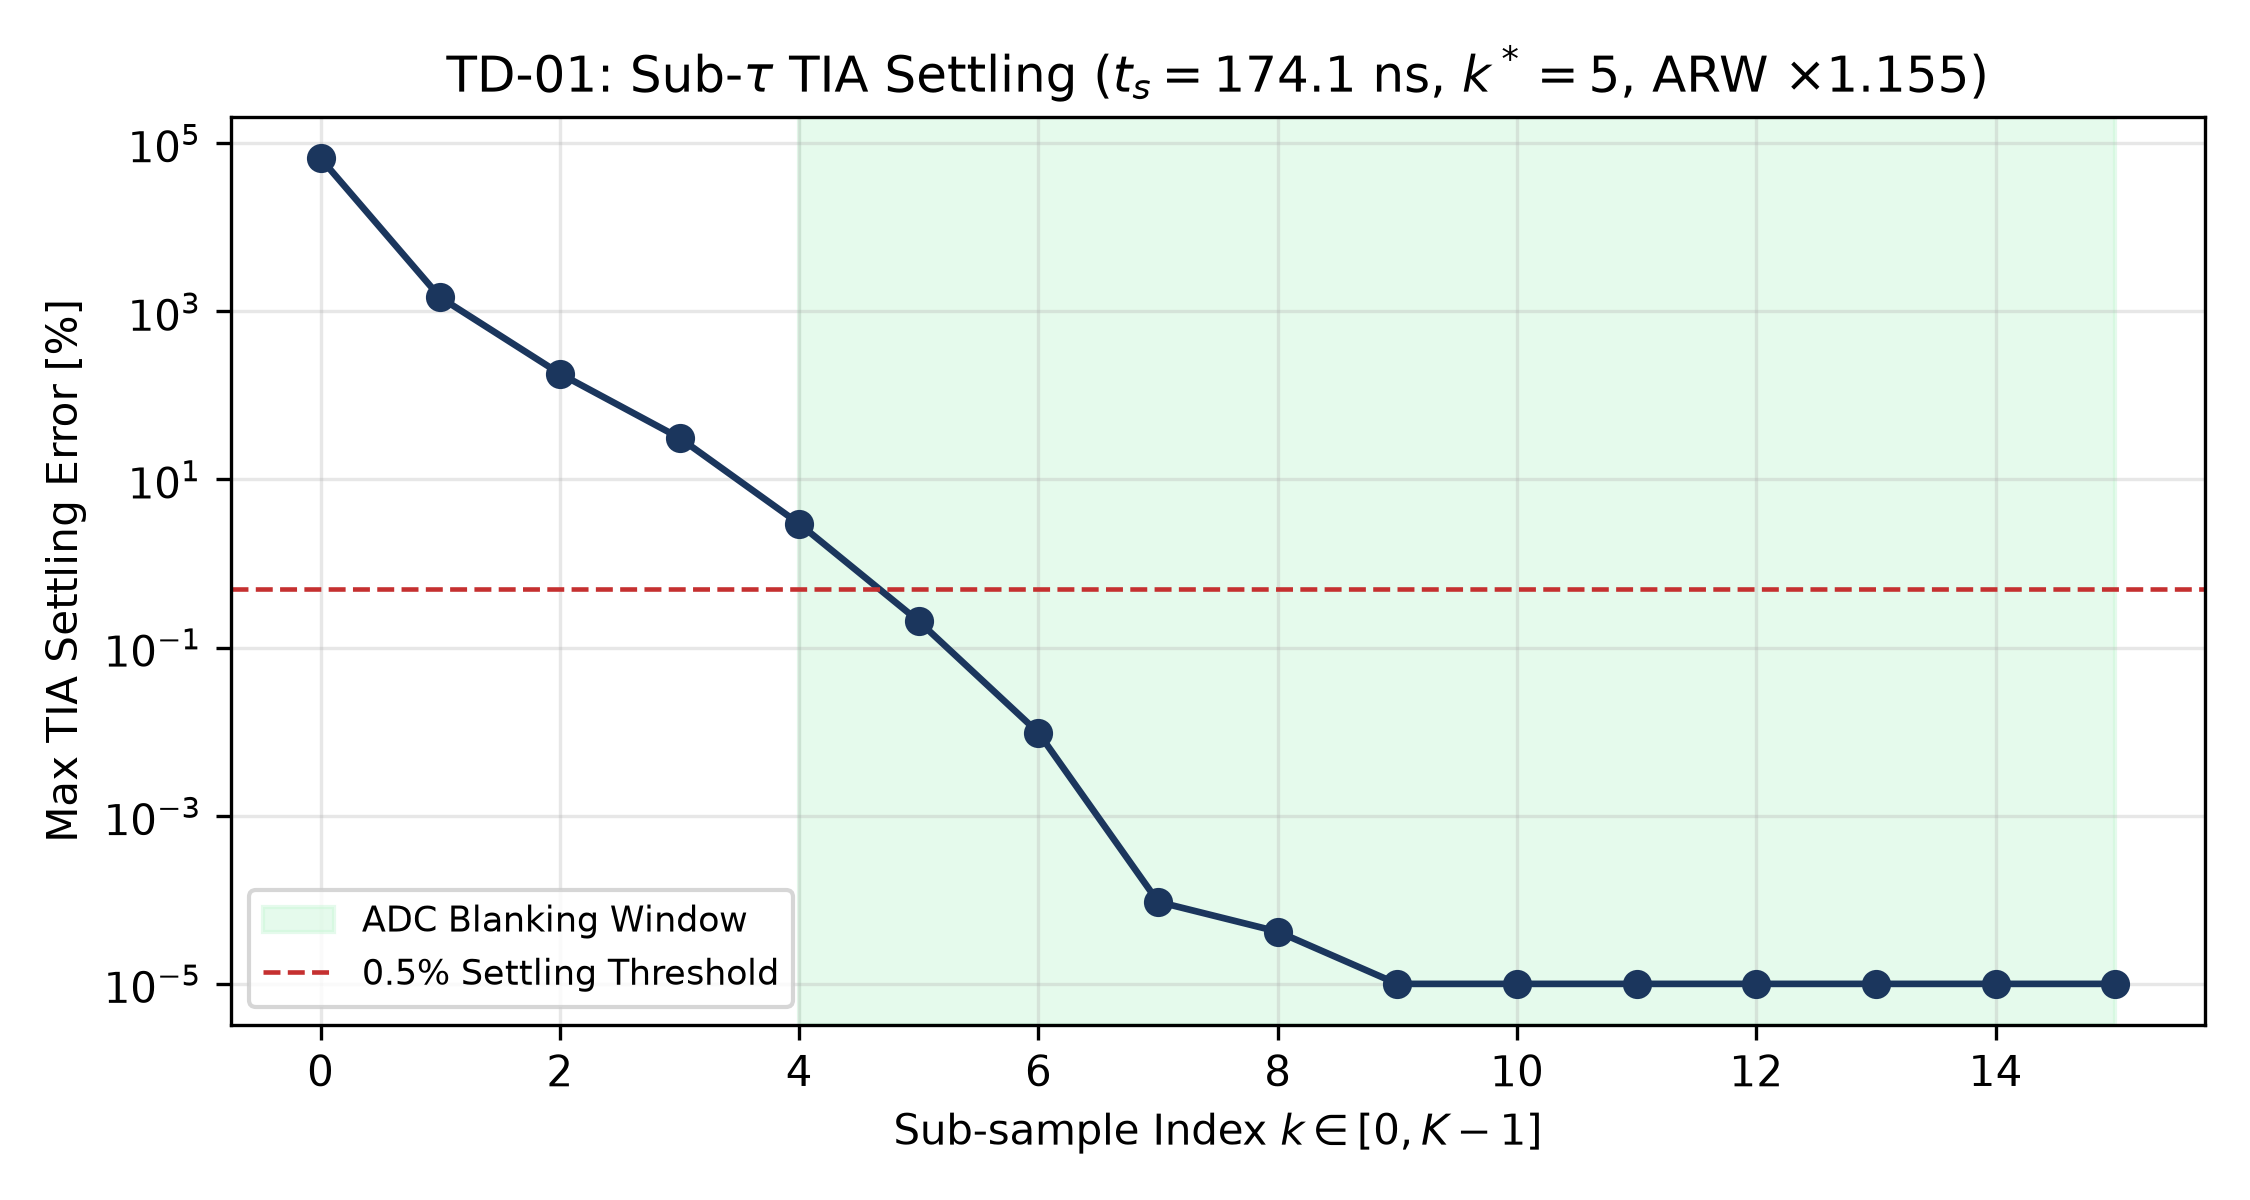
\includegraphics[width=0.88\textwidth,height=0.43\textheight,keepaspectratio]{../examples/full_all_scenarios/figures/td01_blanking.png}
\end{center}
\vspace{0.02cm}
\begin{columns}[T]
  \begin{column}{0.52\textwidth}
    \begin{eqbox}[Cách đọc Đồ thị \& Bản chất Vật lý (LTF TIA)]
      \begin{itemize}\setlength\itemsep{1.6pt}
        \item \textbf{Trục X/Y:} Chỉ số mẫu con $k\in[0,15]$ trong 1 chu kỳ truyền $\tau=4.90\,\mu\text{s}$ vs sai số xác lập cực đại của điện áp TIA [\%] (thang logarit).
        \item \textbf{Bản chất vật lý:} Tại $k=0..3$, gai chuyển mạch DAC + xuyên nhiễu $C_{\text{xtalk}}\dot{V}$ qua LTF $H_{\text{TIA}}(s)$ gây sai số rất lớn ($10^2\text{--}10^5\%$); sau $k=4$ sóng tắt dần xuống dưới ngưỡng đỏ $0.5\%$ (vùng tô xanh \emph{ADC Blanking Window} $[4..15]$).
      \end{itemize}
    \end{eqbox}
  \end{column}
  \begin{column}{0.46\textwidth}
    \begin{remarkbox}[Kết luận Kỹ thuật \& Điều được Chứng minh]
      \begin{itemize}\setlength\itemsep{1.6pt}
        \item Thời gian xác lập TIA $0.1\%$: \textbf{$t_s = 174.1\text{ ns}$}.
        \item Điểm mở cửa sổ Blanking tối ưu: \textbf{$k^*_{\text{start}} = 5$} (sai số vùng sạch \textbf{2.98\%}, hệ số tăng ARW $1/\sqrt{\eta_b}$ chỉ $\times\mathbf{1.155}$).
        \item \textbf{Giá trị:} Định cỡ chính xác số xung nhịp FPGA cần che gai chuyển mạch mà không làm suy giảm tỷ số tín hiệu/nhiễu (SNR).
      \end{itemize}
    \end{remarkbox}
  \end{column}
\end{columns}
\end{frame}

% SLIDE 19: THỰC NGHIỆM (2/11) — DYN-01: ĐÁP ỨNG BƯỚC VÒNG KÍN
\begin{frame}{Kết quả Thực nghiệm (2/11): Đáp ứng Bước Vòng kín (Step Response)}{\texttt{DYN-01} (\texttt{dyn01\_step\_response.png}) \enspace|\enspace Nhảy bậc $0\to 10^\circ/\text{s}$ \& $100^\circ/\text{s}$ (4-State vs 6-State \& quét $K_{\text{tot},1}$)}
\begin{columns}[c]
  \begin{column}{0.66\textwidth}
    \centering
    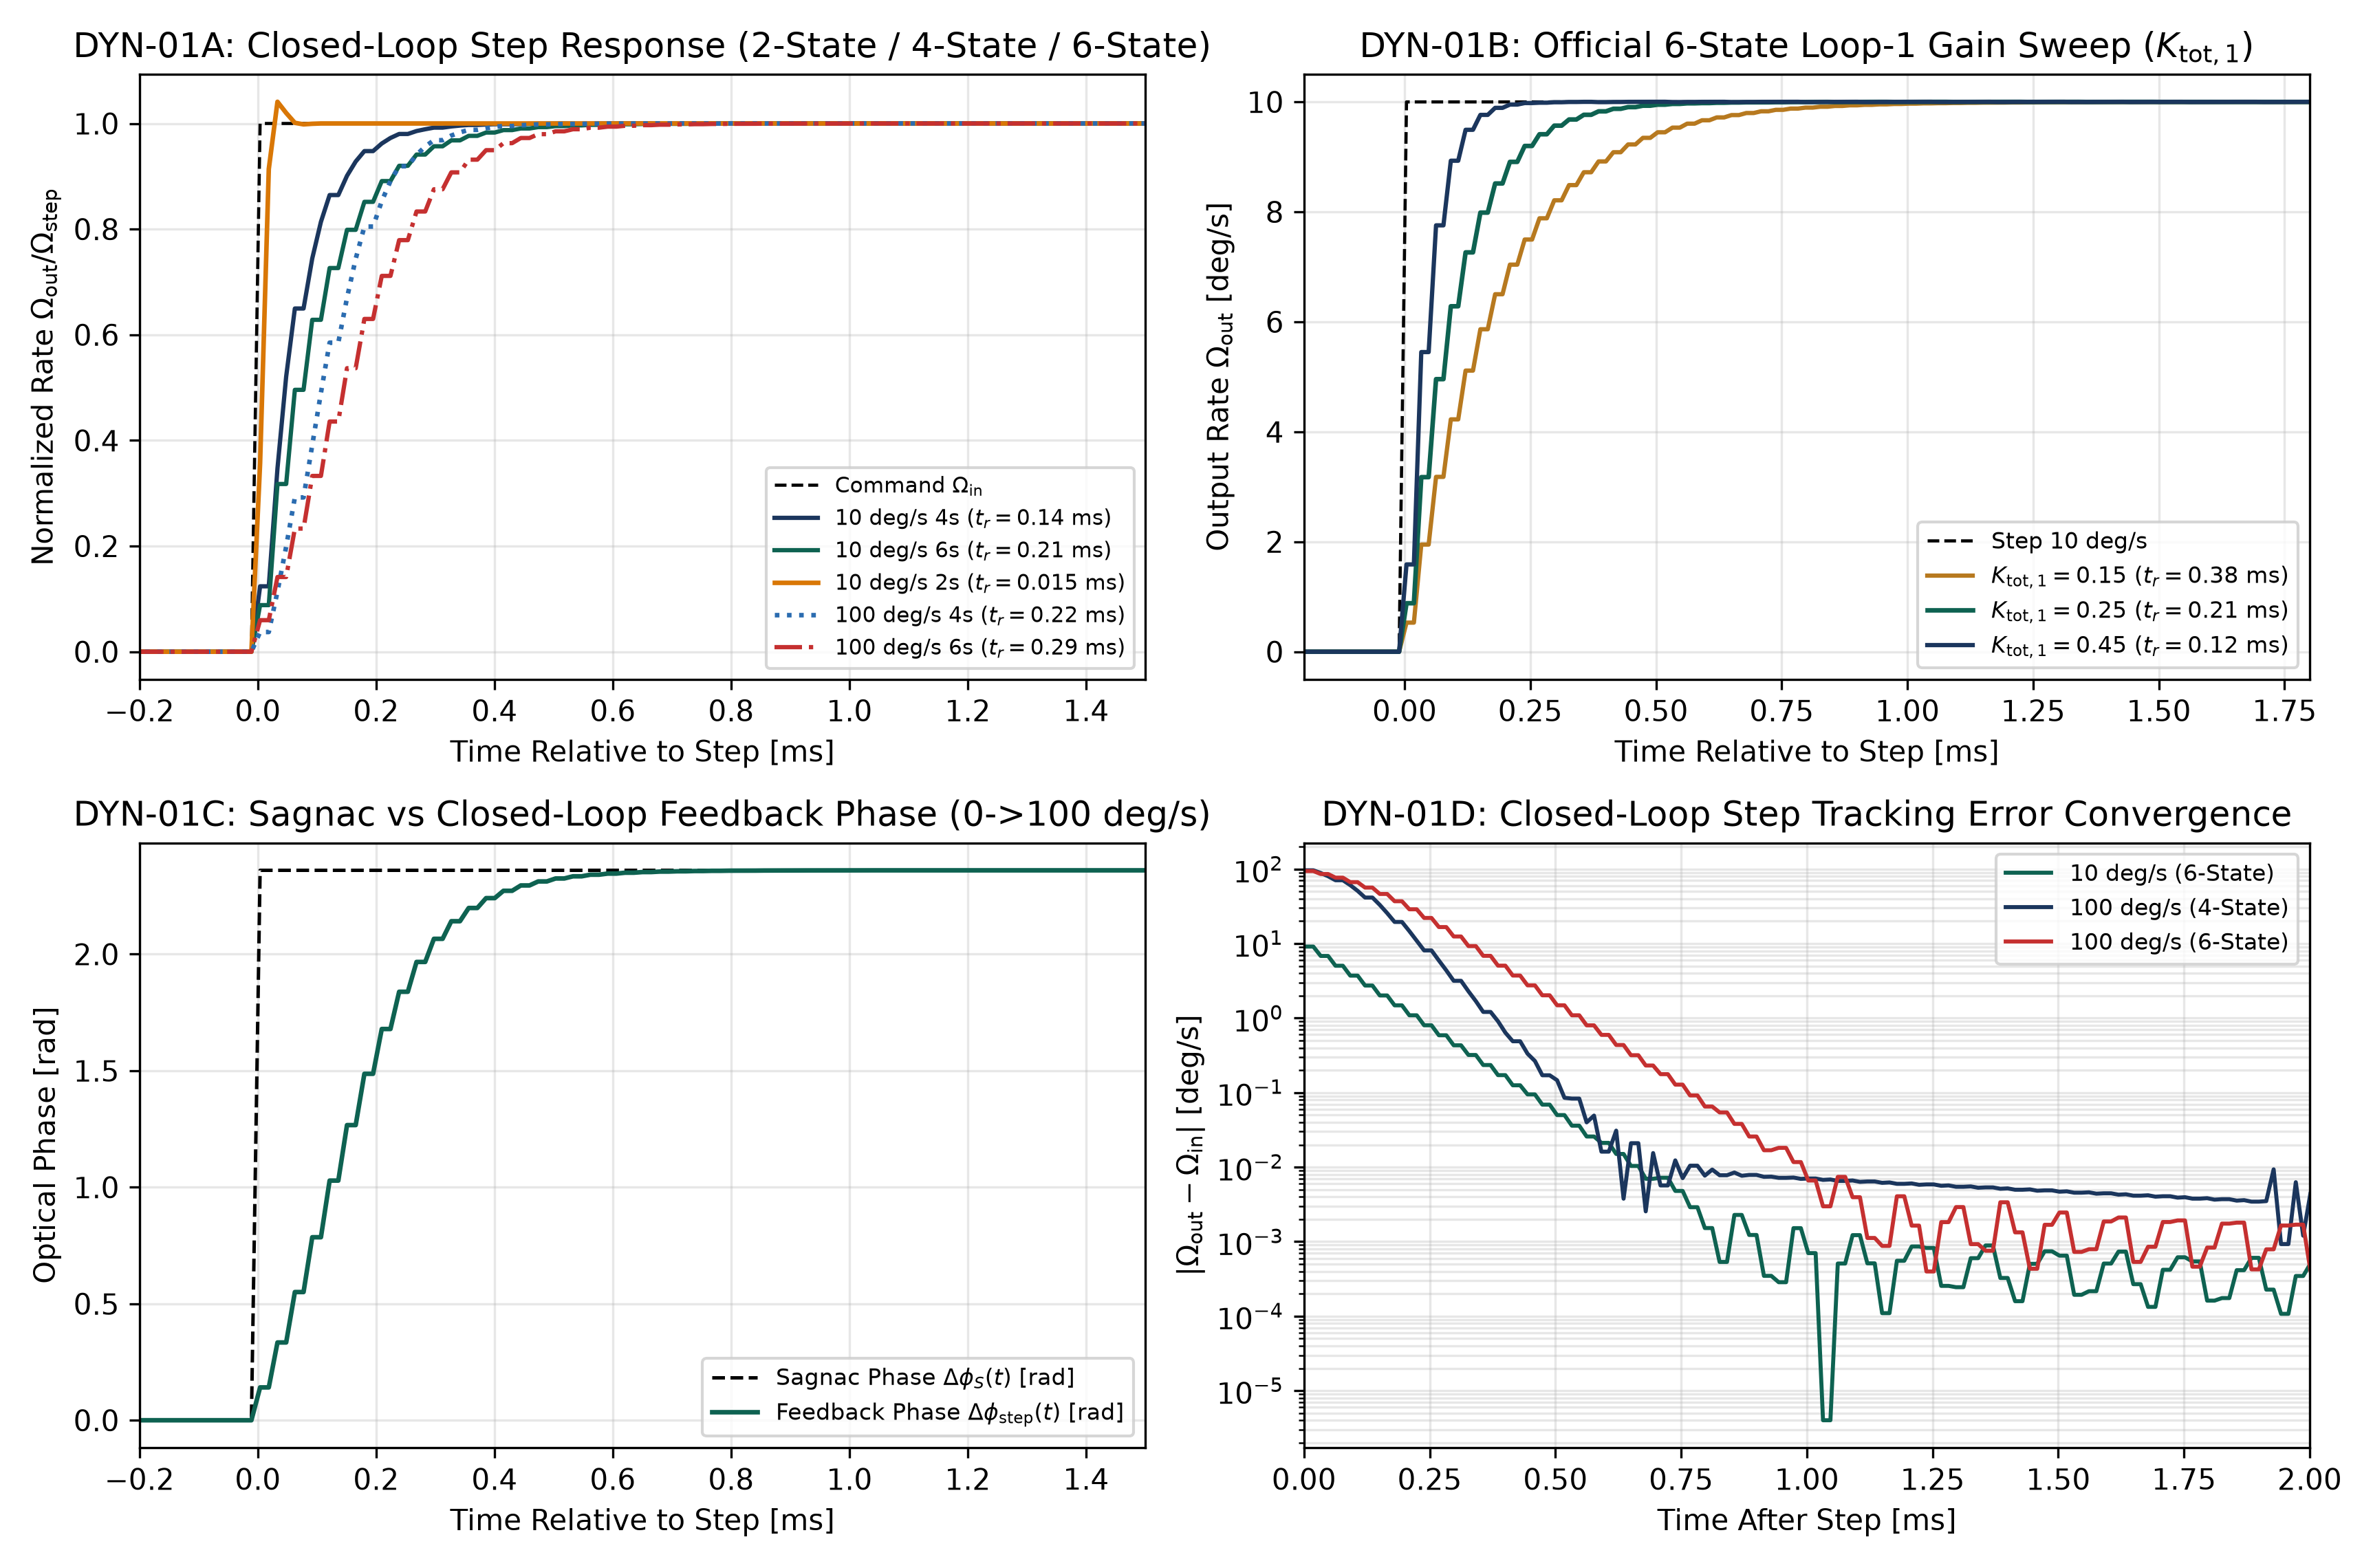
\includegraphics[width=\linewidth,height=0.77\textheight,keepaspectratio]{../examples/full_all_scenarios/figures/dyn01_step_response.png}
  \end{column}
  \begin{column}{0.32\textwidth}
    \begin{eqbox}[Giải thích Đồ thị \& Ý nghĩa Vật lý]
      \begin{itemize}\setlength\itemsep{2.8pt}
        \item \textbf{Cách đọc:} Trục hoành là thời gian [ms]; đường nét đứt là tốc độ góc bước nhảy đầu vào $\Omega_{\text{in}}(t)$; các đường màu là đầu ra vòng kín $\Omega_{\text{out}}(t)$ khi đổi kiến trúc DSP và hệ số vòng $K_{\text{tot},1}$.
        \item \textbf{Bản chất vật lý:} Hệ tích phân loại I với trễ pipeline $d=2$ ($L_1(z)=K_{\text{tot},1}/[z^2(z-1)]$) quyết định trực tiếp độ nhanh ($t_r$) và mức vọt lố (OS): tăng $K_{\text{tot},1}$ làm vòng phản hồi nhanh hơn nhưng tiến gần biên ổn định Jury.
        \item \textbf{Chứng minh (6-State chuẩn):} Thời gian tăng $t_r = \mathbf{0.206\text{ ms}}$ ($10^\circ/\text{s}$) và $\mathbf{0.294\text{ ms}}$ ($100^\circ/\text{s}$), độ vọt lố \textbf{0.00\%}, sai số xác lập \textbf{0.0000\%} (bám tuyệt đối không sai số tĩnh).
      \end{itemize}
    \end{eqbox}
  \end{column}
\end{columns}
\end{frame}

% SLIDE 20: THỰC NGHIỆM (3/11) — DYN-02: ĐÁP ỨNG TẦN SỐ (BODE MAG, PHASE & GROUP DELAY)
\begin{frame}{Kết quả Thực nghiệm (3/11): Đáp ứng Tần số Vòng kín (Bode \& Group Delay)}{\texttt{DYN-02} (\texttt{dyn02\_freq\_response.png}) \enspace|\enspace Quét 15 tần số $10\text{ Hz}\dots 5\text{ kHz}$: Biên độ, Pha \& Độ trễ nhóm}
\begin{columns}[c]
  \begin{column}{0.64\textwidth}
    \centering
    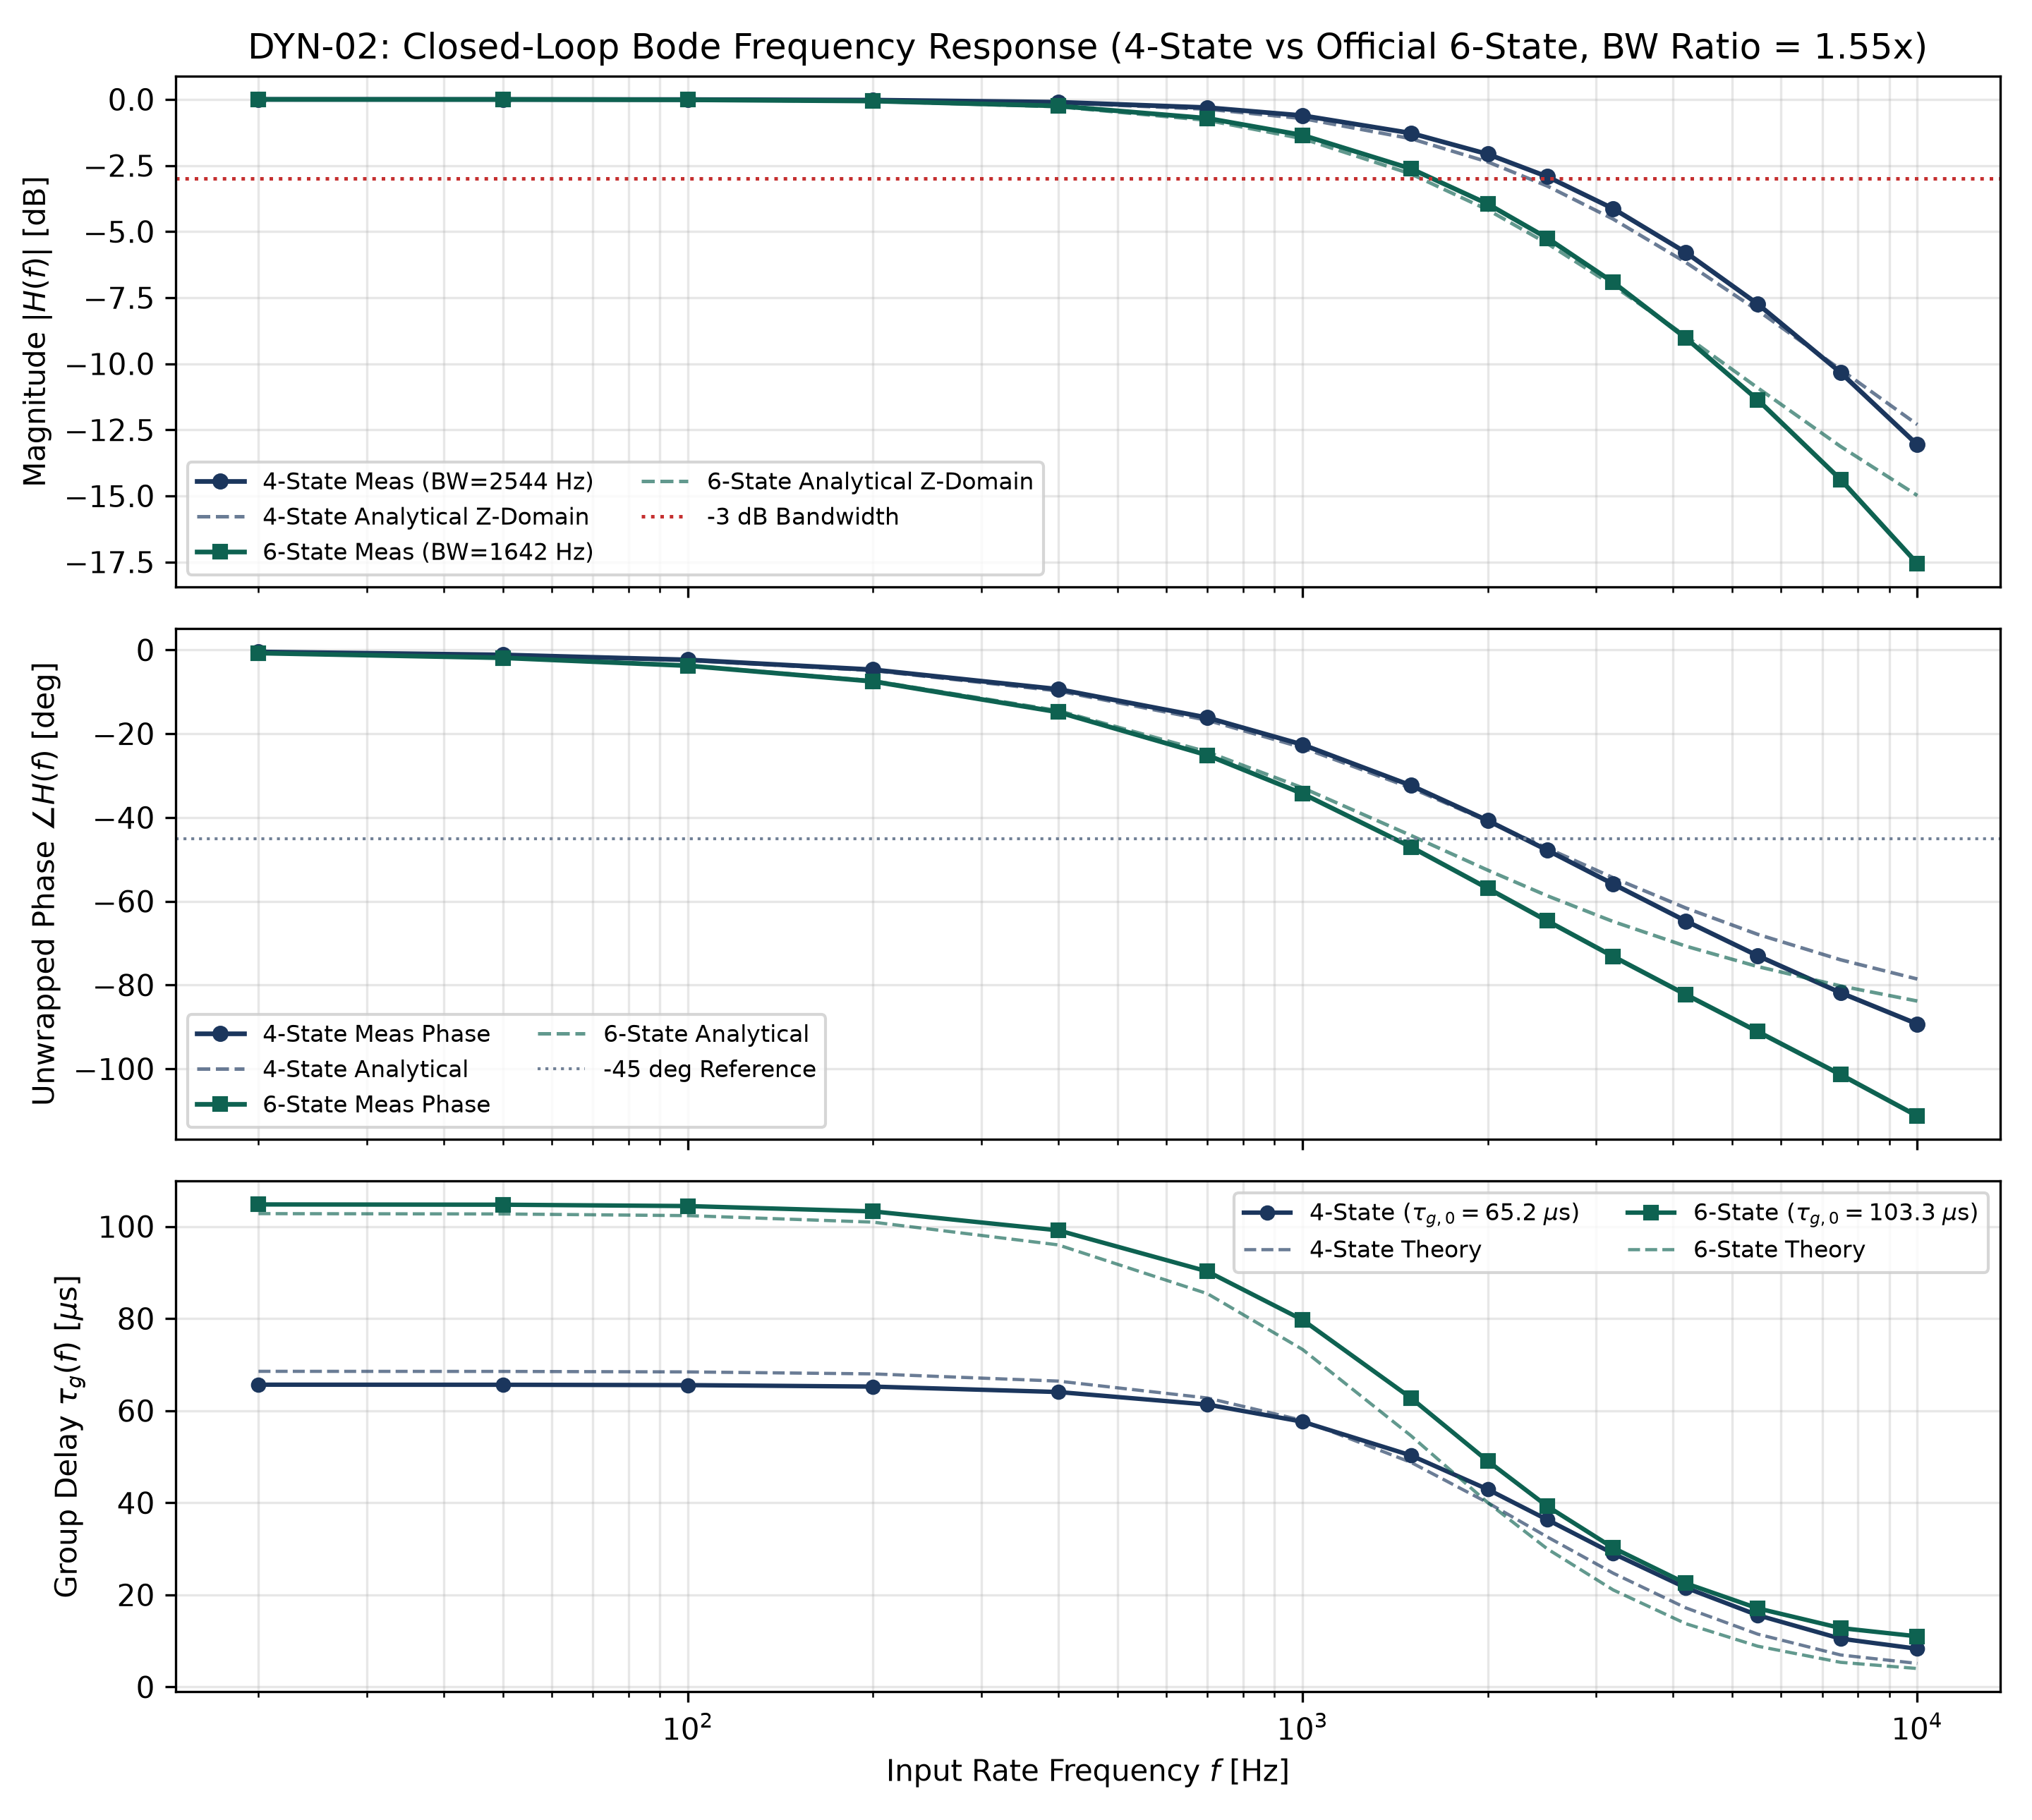
\includegraphics[width=\linewidth,height=0.79\textheight,keepaspectratio]{../examples/full_all_scenarios/figures/dyn02_freq_response.png}
  \end{column}
  \begin{column}{0.34\textwidth}
    \begin{remarkbox}[Giải thích 3 Đồ thị Bode \& Ý nghĩa]
      \begin{itemize}\setlength\itemsep{2.6pt}
        \item \textbf{Trên (Biên độ [dB]):} Tỷ số $|\Omega_{\text{out}}/\Omega_{\text{in}}|$ phẳng $0\text{ dB}$ ở tần số thấp và giảm $-3\text{ dB}$ tại băng thông vòng kín $f_{-3\text{ dB}}$ (đặc tính lọc thông thấp của bộ tích phân số).
        \item \textbf{Giữa (Pha [deg]):} Góc trễ pha tăng dần theo tần số do trễ khung điều biến ($4\tau$ hoặc $6\tau$) cộng trễ pipeline $d=2$.
        \item \textbf{Dưới (Trễ nhóm $\tau_g=-\frac{d\phi}{d\omega}$):} Đo độ trễ truyền tín hiệu thực tới máy tính dẫn đường GNC.
        \item \textbf{Chứng minh định lượng:} 4-State đạt \textbf{$f_{-3\text{dB}}=2544\text{ Hz}$} ($\tau_g=65.2\,\mu\text{s}$), 6-State đạt \textbf{$1642\text{ Hz}$} ($\tau_g=103.3\,\mu\text{s}$); tỷ số thực đo \textbf{$1.55\times$} khớp sát tỷ số khung lý thuyết $6\tau/4\tau = 1.50\times$.
      \end{itemize}
    \end{remarkbox}
  \end{column}
\end{columns}
\end{frame}

% SLIDE 21: THỰC NGHIỆM (4/11) — DYN-03: PHỔ PSD ĐẦU RA & NHIỄU RMS TÍCH LŨY
\begin{frame}{Kết quả Thực nghiệm (4/11): Phổ Mật độ Công suất Đầu ra (Output PSD / ASD)}{\texttt{DYN-03} (\texttt{dyn03\_output\_psd.png}) \enspace|\enspace Phân bố năng lượng nhiễu theo tần số \& Kiểm chứng nền ARW}
\begin{center}
  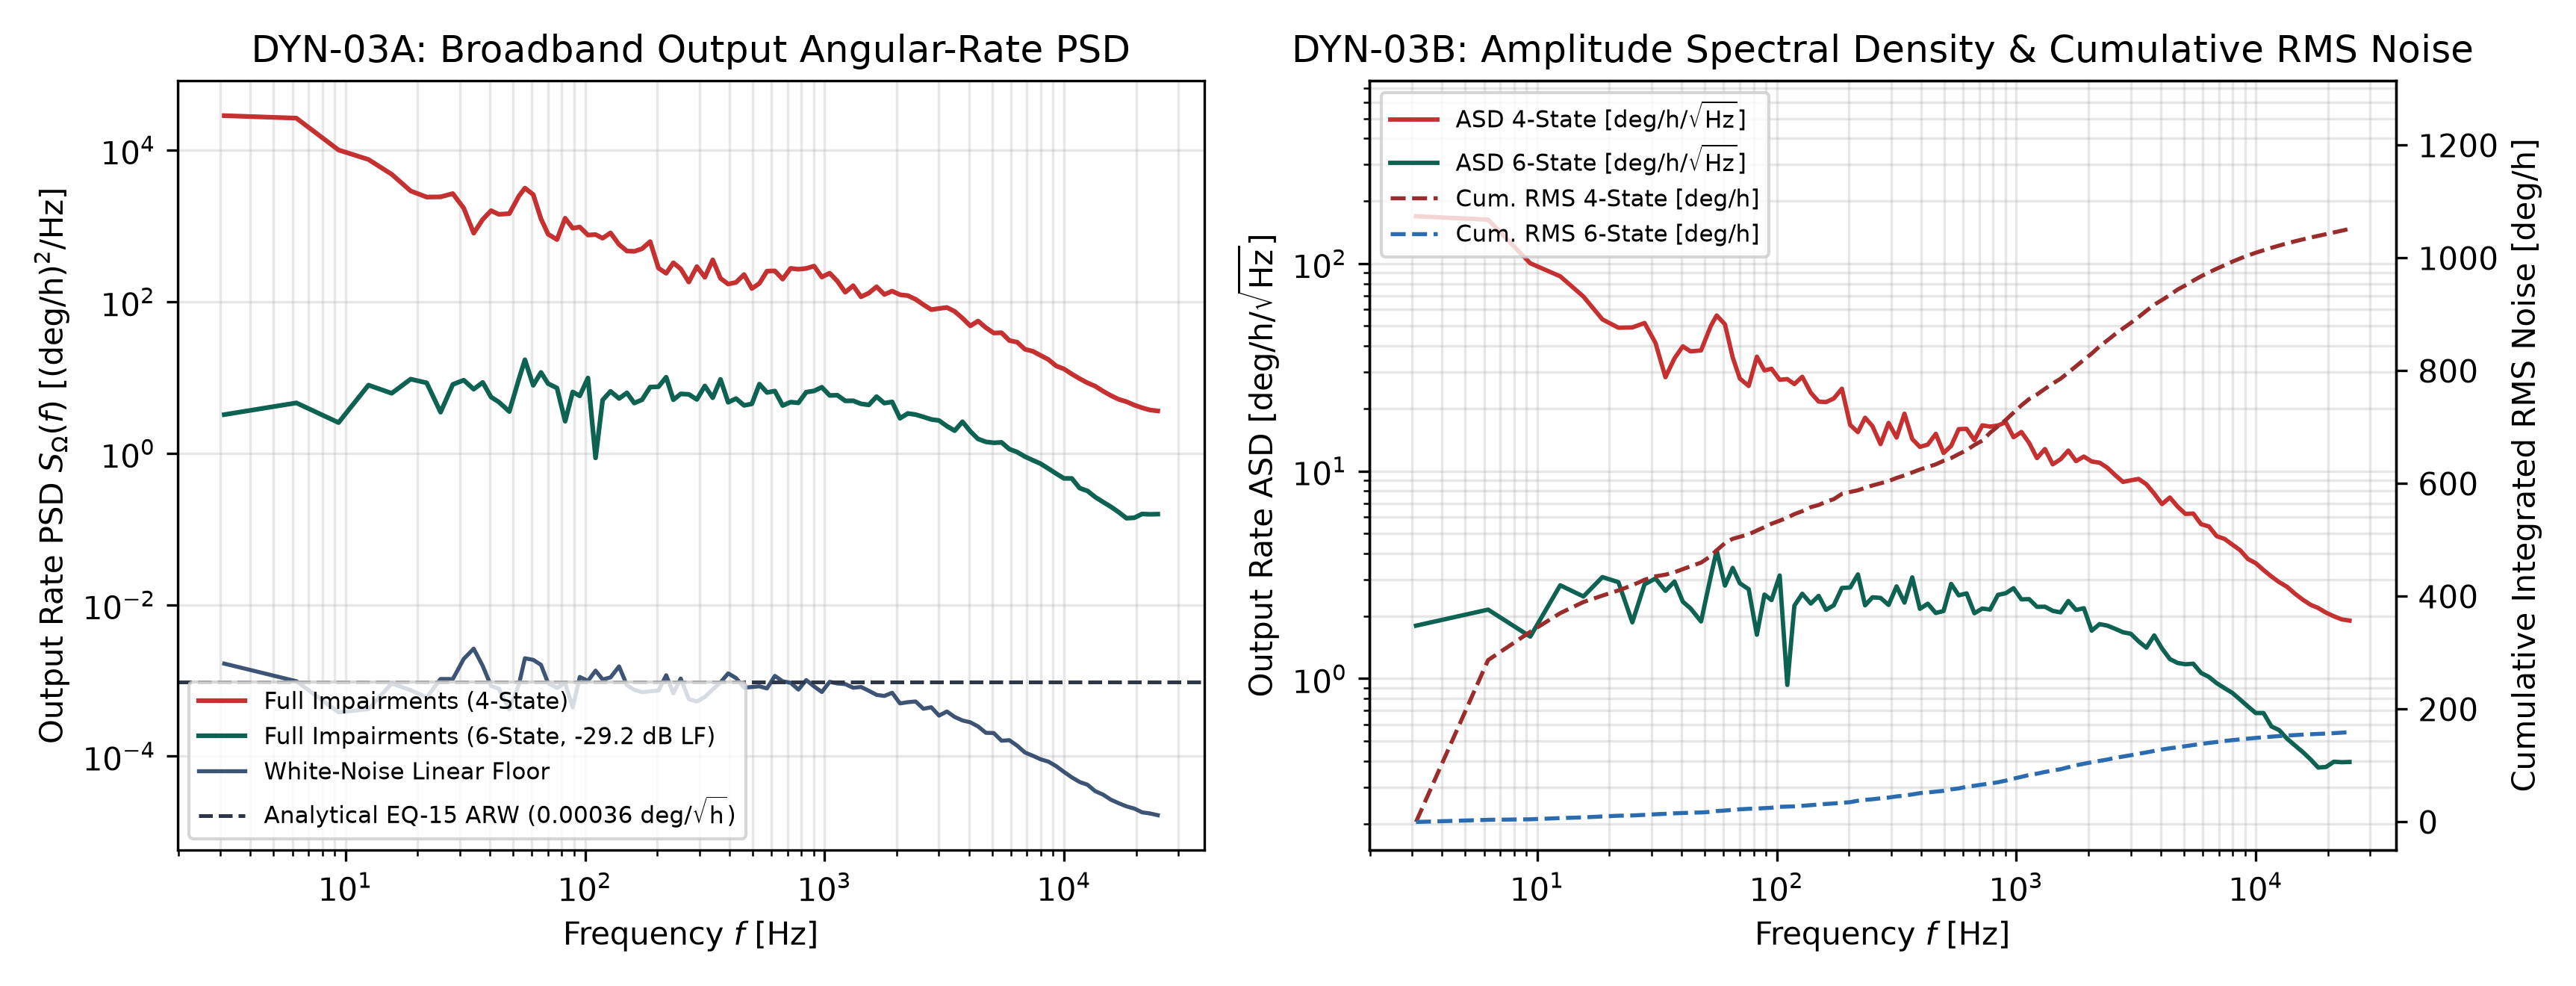
\includegraphics[width=0.94\textwidth,height=0.43\textheight,keepaspectratio]{../examples/full_all_scenarios/figures/dyn03_output_psd.png}
\end{center}
\vspace{0.02cm}
\begin{columns}[T]
  \begin{column}{0.51\textwidth}
    \begin{eqbox}[Cách đọc Đồ thị \& Bản chất Vật lý]
      \begin{itemize}\setlength\itemsep{1.6pt}
        \item \textbf{Hình trái (PSD $[(^\circ/\text{h})^2/\text{Hz}]$):} Đường đỏ (4-State) mang sườn $1/f$ cao ở tần số thấp do rò ký sinh; đường xanh (6-State) triệt mạnh tần thấp; đường xanh đậm nằm sát nền nhiễu trắng giải tích \texttt{EQ-15} và dốc xuống khi $f > f_{-3\text{dB}}$.
        \item \textbf{Hình phải (ASD \& Nhiễu RMS tích lũy):} Đường liền nét là phổ biên độ ASD; đường nét đứt (trục phải) cho tổng nhiễu RMS tích lũy theo băng thông $[f_{\min},f]$.
      \end{itemize}
    \end{eqbox}
  \end{column}
  \begin{column}{0.47\textwidth}
    \begin{remarkbox}[Kết luận Kỹ thuật \& Điều được Chứng minh]
      \begin{itemize}\setlength\itemsep{1.6pt}
        \item Nền trắng đo từ phổ PSD khớp lý thuyết ARW $= \mathbf{0.0004^\circ/\sqrt{\text{h}}}$ (tỷ số thực đo/lý thuyết $= \mathbf{0.97}$).
        \item Kiến trúc 6-State triệt tiêu nhiễu tần thấp vượt trội \textbf{$29.2\text{ dB}$} so với 4-State và tự lọc suy giảm tần cao \textbf{$-13.5\text{ dB}$}.
        \item \textbf{Chứng minh:} Đảm bảo tính nhất quán tuyệt đối giữa miền tần số (PSD) và miền thời gian (Allan Variance).
      \end{itemize}
    \end{remarkbox}
  \end{column}
\end{columns}
\end{frame}

% SLIDE 22: THỰC NGHIỆM (5/11) — DYN-04: CHUỖI ĐIỆN–QUANG HÌNH SIN
\begin{frame}{Kết quả Thực nghiệm (5/11): Soi Toàn chuỗi Điện–Quang Dưới Kích thích Hình Sin}{\texttt{DYN-04} (\texttt{dyn04\_sine\_electro\_optic.png}) \enspace|\enspace $\Omega_{\text{in}}(t) = 50^\circ/\text{s}\,\sin(2\pi\cdot 250t)$ qua 6 nút vật lý}
\begin{columns}[c]
  \begin{column}{0.68\textwidth}
    \centering
    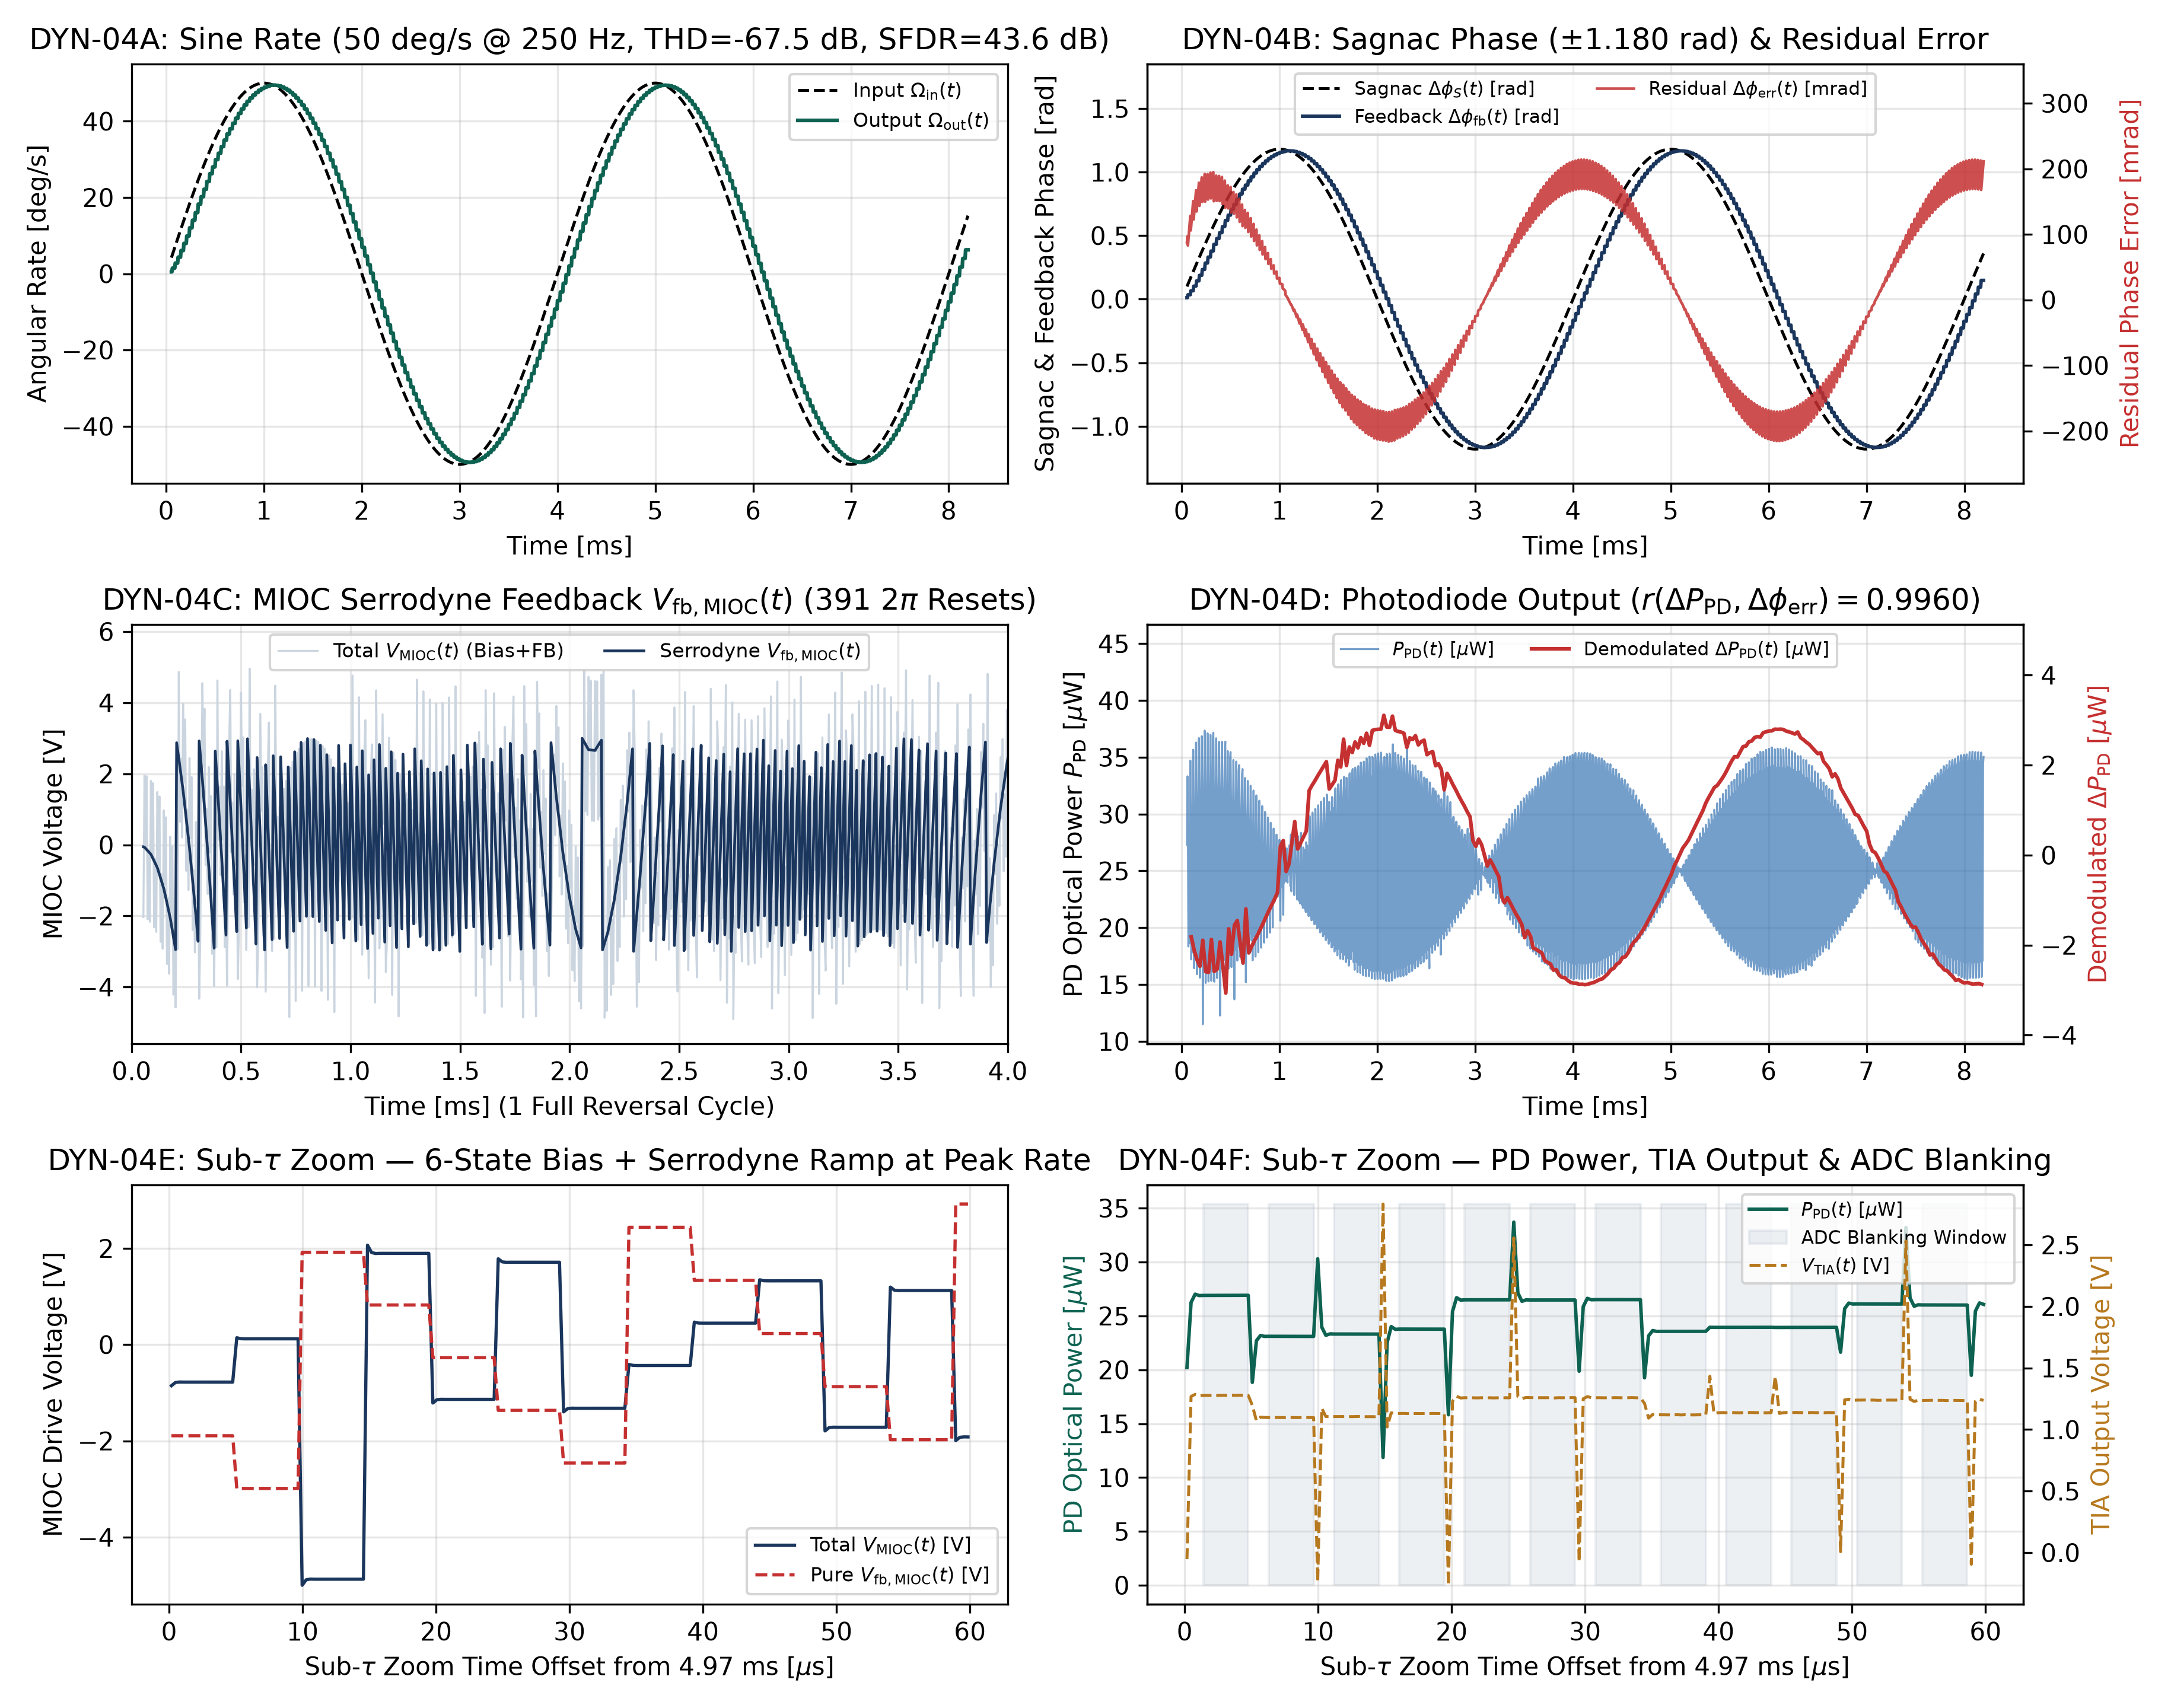
\includegraphics[width=\linewidth,height=0.79\textheight,keepaspectratio]{../examples/full_all_scenarios/figures/dyn04_sine_electro_optic.png}
  \end{column}
  \begin{column}{0.30\textwidth}
    \begin{remarkbox}[Hướng dẫn Đọc 6 Biểu đồ (A–F)]
      \begin{itemize}\setlength\itemsep{2.4pt}
        \item \textbf{A (Tốc độ góc):} Đầu ra $\Omega_{\text{out}}$ bám khít sóng sin $250\text{ Hz}$ (THD \textbf{$-67.5\text{ dB}$}, SFDR \textbf{$43.6\text{ dB}$}), chứng tỏ vòng kín không méo hài.
        \item \textbf{B (Pha Sagnac vs Hồi tiếp):} Pha $\Delta\phi_S=\pm 1.18\text{ rad}$ bị pha bù triệt tiêu sát $0$ (đường đỏ pha dư cực nhỏ).
        \item \textbf{C (Điện áp MIOC $V_{\text{fb}}$):} Xuất hiện dạng răng cưa \emph{serrodyne} với \textbf{391 lần reset $2\pi$} mượt mà khi pha vượt biên.
        \item \textbf{D (Công suất Photodiode):} Sóng mang cao tần điều biên theo pha dư với hệ số tương quan $r=\mathbf{0.9960}$.
        \item \textbf{E \& F (Zoom sub-$\tau$):} Soi cận cảnh 6 bậc điều biến, gai TIA và vùng tô xám cửa sổ ADC Blanking.
      \end{itemize}
    \end{remarkbox}
  \end{column}
\end{columns}
\end{frame}

% SLIDE 23: THỰC NGHIỆM (6/11) — GATE 2: DEADBAND & BUNNY EARS
\begin{frame}{Kết quả Thực nghiệm (6/11): Khử Vùng chết (Deadband) \& Lỗi Tỷ lệ Bunny Ears}{Gate 2 (\texttt{bunny\_ears.png}) \enspace|\enspace Quét 23 điểm tốc độ siêu chậm $\Omega_{\text{in}}\in[-0.5,+0.5]^\circ/\text{s}$}
\begin{columns}[c]
  \begin{column}{0.67\textwidth}
    \centering
    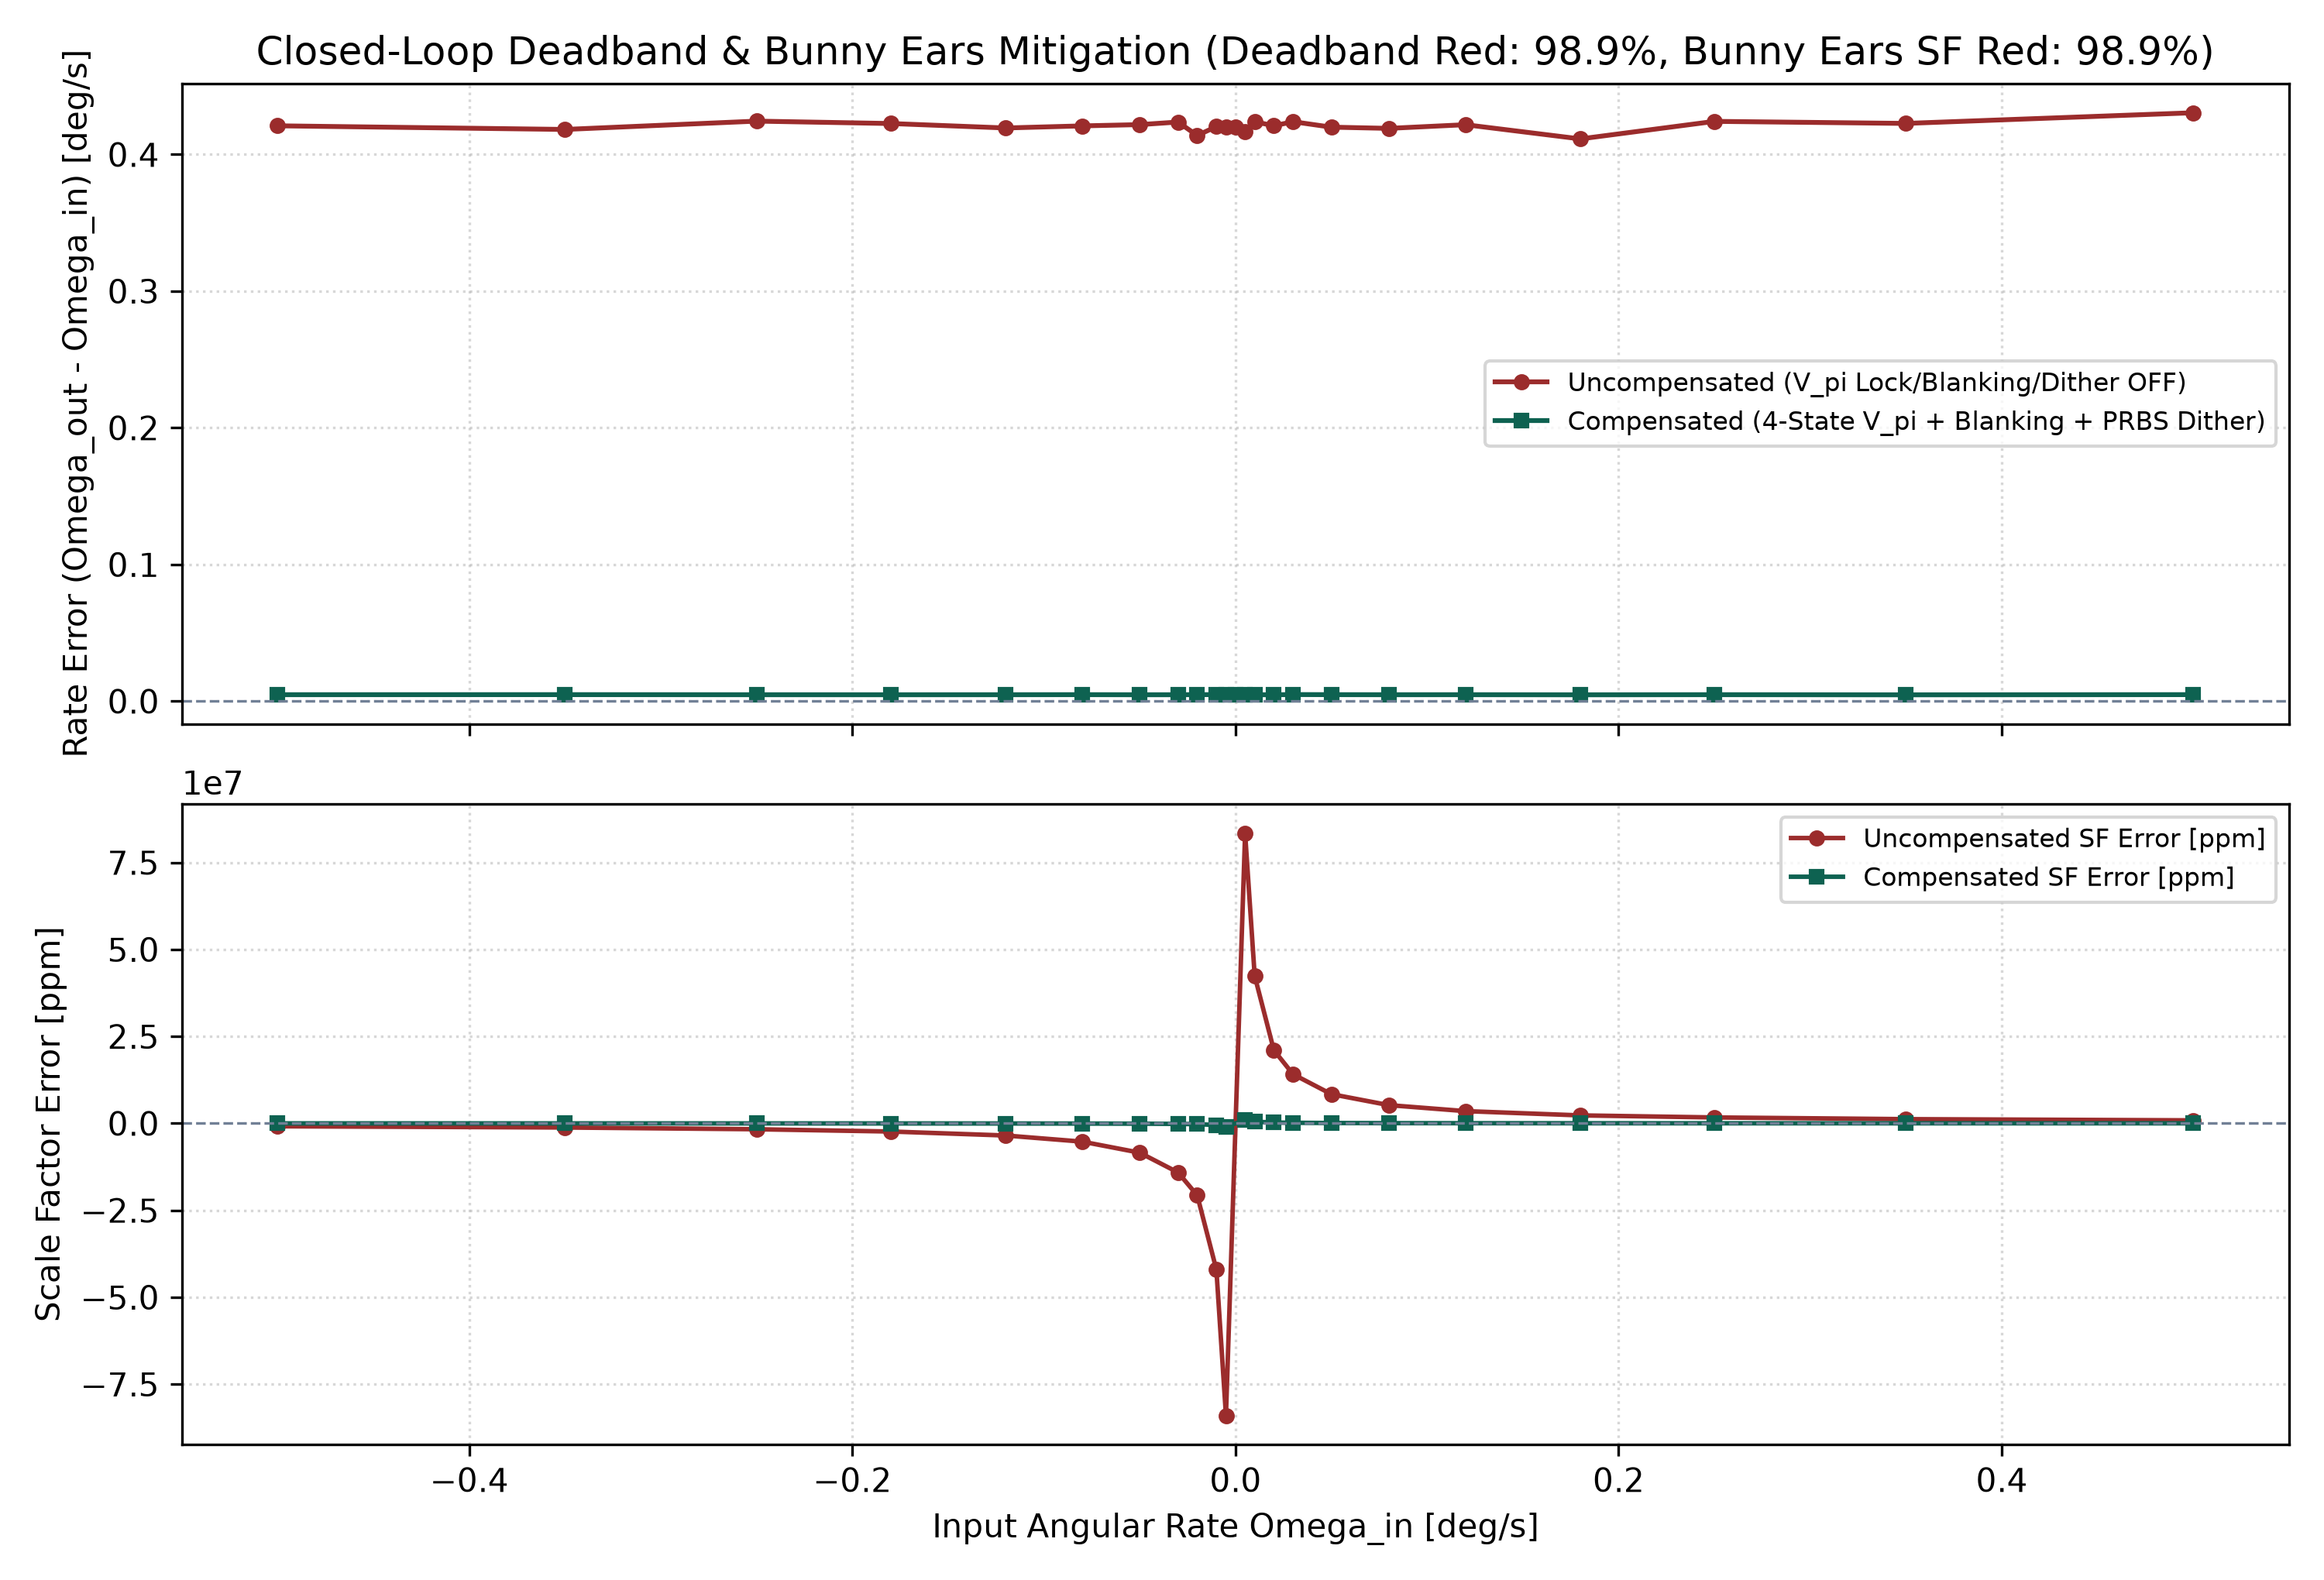
\includegraphics[width=\linewidth,height=0.77\textheight,keepaspectratio]{../examples/full_all_scenarios/figures/bunny_ears.png}
  \end{column}
  \begin{column}{0.31\textwidth}
    \begin{eqbox}[Hướng dẫn Đọc Đồ thị Gate 2]
      \begin{itemize}\setlength\itemsep{2.6pt}
        \item \textbf{Đồ thị trên (Sai số tốc độ góc):} Trục X là vận tốc quay thực quanh $0$; trục Y là sai số $|\Omega_{\text{out}}-\Omega_{\text{in}}|$.
        \item \textbf{Đồ thị dưới (Lỗi hệ số tỷ lệ [ppm]):} Khi tắt bù (đường đỏ), xuyên nhiễu PCB khóa dính vòng hồi tiếp quanh $0$ rồi bật vọt tạo hai đỉnh nhọn đối xứng gọi là \emph{Tai thỏ (Bunny Ears)}.
        \item \textbf{Đường xanh (Bật Vòng 2 + Blanking + PRBS dither):} Nằm phẳng sát trục $0$ trên toàn dải đo.
        \item \textbf{Chứng minh:} Giảm \textbf{98.85\%} đỉnh Deadband và \textbf{98.85\%} lỗi Bunny Ears (vượt chuẩn $\ge 90\%$).
      \end{itemize}
    \end{eqbox}
  \end{column}
\end{columns}
\end{frame}

% SLIDE 24: THỰC NGHIỆM (7/11) — GATE 4: ALLAN VARIANCE 5 VÙNG (10 GIỜ)
\begin{frame}{Kết quả Thực nghiệm (7/11): Biểu đồ Allan Variance 5 Vùng Chế độ Kép (10 Giờ)}{Gate 4 (\texttt{avar\_5regions.png}) \enspace|\enspace Ghép nối $4\times 60\text{ s}$ SystemC-AMS (Tầng 2) + $12\times 10\text{ h}$ @ $100\text{ Hz}$ (Tầng 3)}
\begin{columns}[c]
  \begin{column}{0.67\textwidth}
    \centering
    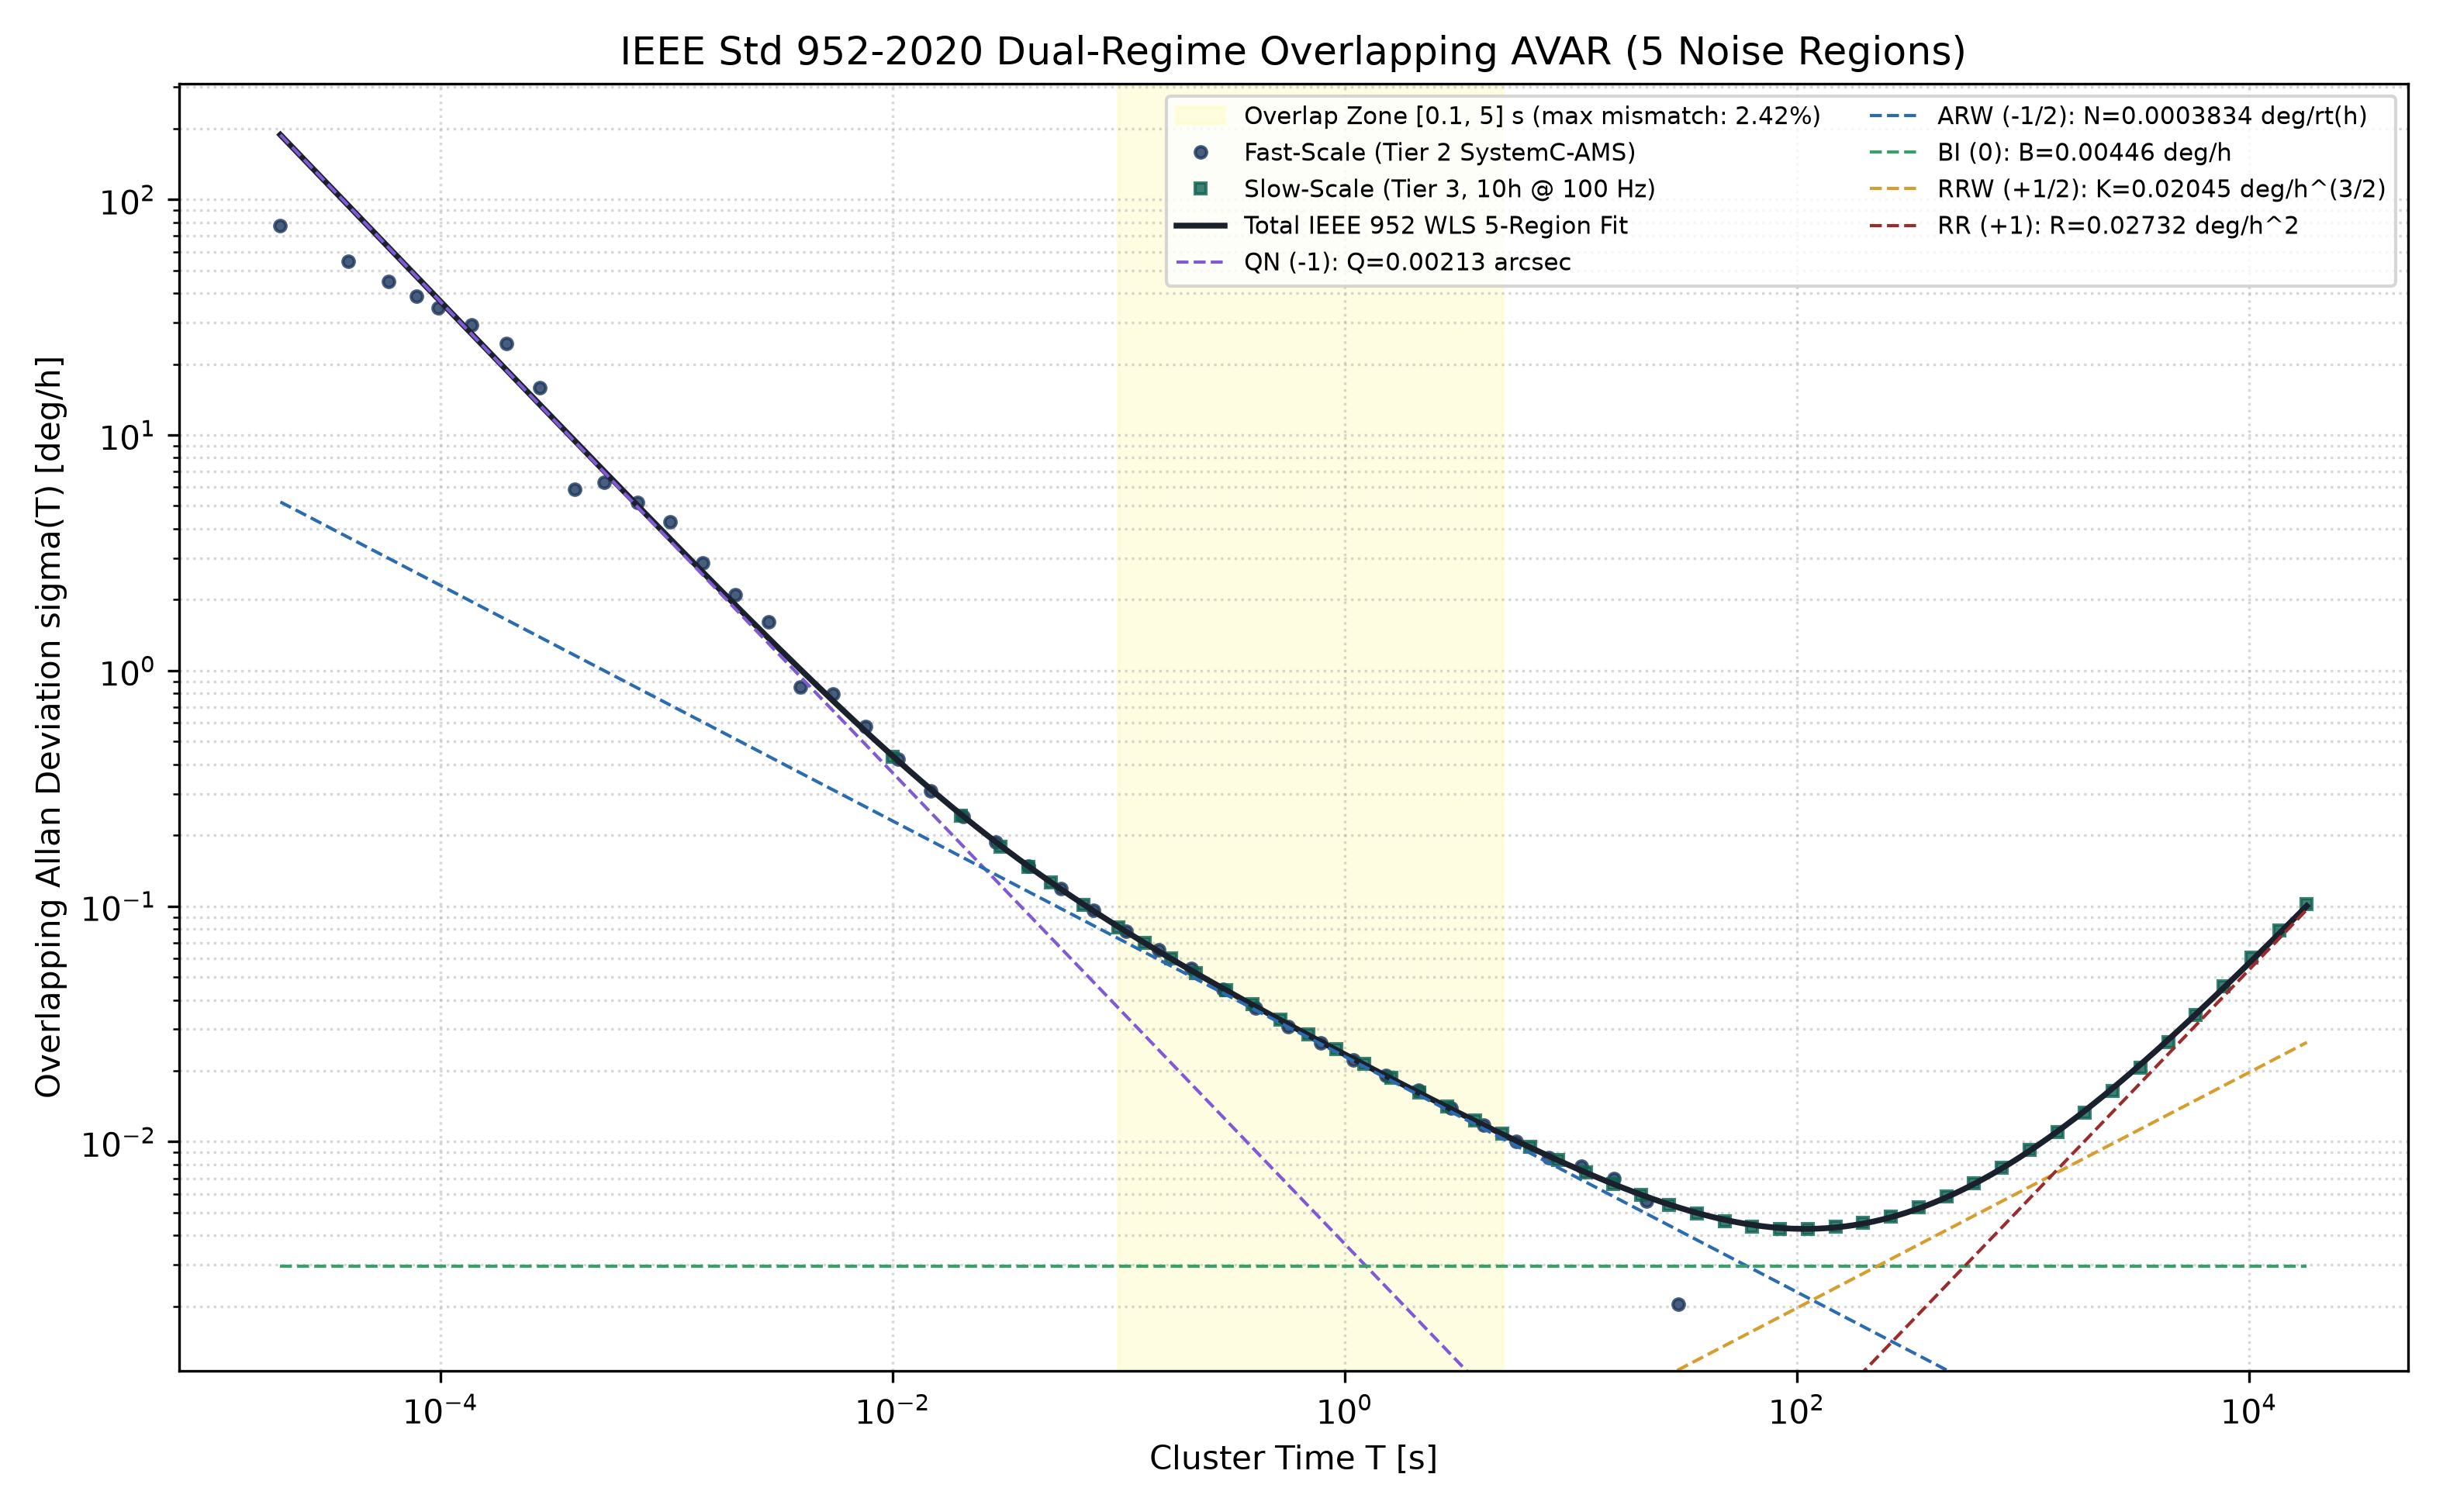
\includegraphics[width=\linewidth,height=0.78\textheight,keepaspectratio]{../examples/full_all_scenarios/figures/avar_5regions.png}
  \end{column}
  \begin{column}{0.31\textwidth}
    \begin{remarkbox}[Cách đọc Biểu đồ Chữ U IEEE 952]
      \begin{itemize}\setlength\itemsep{2.2pt}
        \item \textbf{Trục X/Y (log--log):} Thời gian lấy trung bình $T_m$ [$10^{-5}\dots 10^4\text{ s}$] vs độ bất ổn định $\sigma(T_m)$ [$^\circ/\text{h}$].
        \item \textbf{5 đoạn dốc lý thuyết:}
          \begin{itemize}\setlength\itemsep{0.6pt}
            \item Dốc $-1$: Lượng tử $Q=0.00213''$
            \item Dốc $-\frac{1}{2}$: ARW $N=0.00383^\circ/\sqrt{\text{h}}$
            \item Đáy phẳng $0$: BI $B=0.00446^\circ/\text{h}$
            \item Dốc $+\frac{1}{2}$: RRW $K=0.02045^\circ/\text{h}^{3/2}$
            \item Dốc $+1$: Trôi nhiệt $R=0.02732^\circ/\text{h}^2$
          \end{itemize}
        \item \textbf{Vùng tô vàng $[0.1,5]\text{ s}$:} Chấm xanh đậm (Tầng 2) và xanh lục (Tầng 3) nối khít nhau với sai lệch \textbf{2.42\%} ($<5\%$), chứng minh phép ghép 11 bậc thang thời gian bảo toàn vật lý.
      \end{itemize}
    \end{remarkbox}
  \end{column}
\end{columns}
\end{frame}

% SLIDE 25: THỰC NGHIỆM (8/11) — GATE 5: SO SÁNH 6-STATE vs 4-STATE DSP
\begin{frame}{Kết quả Thực nghiệm (8/11): Thực nghiệm Khử Nhiễu Ký sinh — 6-State vs 4-State}{Gate 5 (\texttt{dsp6\_compare.png}) \enspace|\enspace Kiểm chứng thực tế độ lợi $+136.94\text{ dB}$ và giảm $-33.3\%$ áp đỉnh MIOC}
\begin{center}
  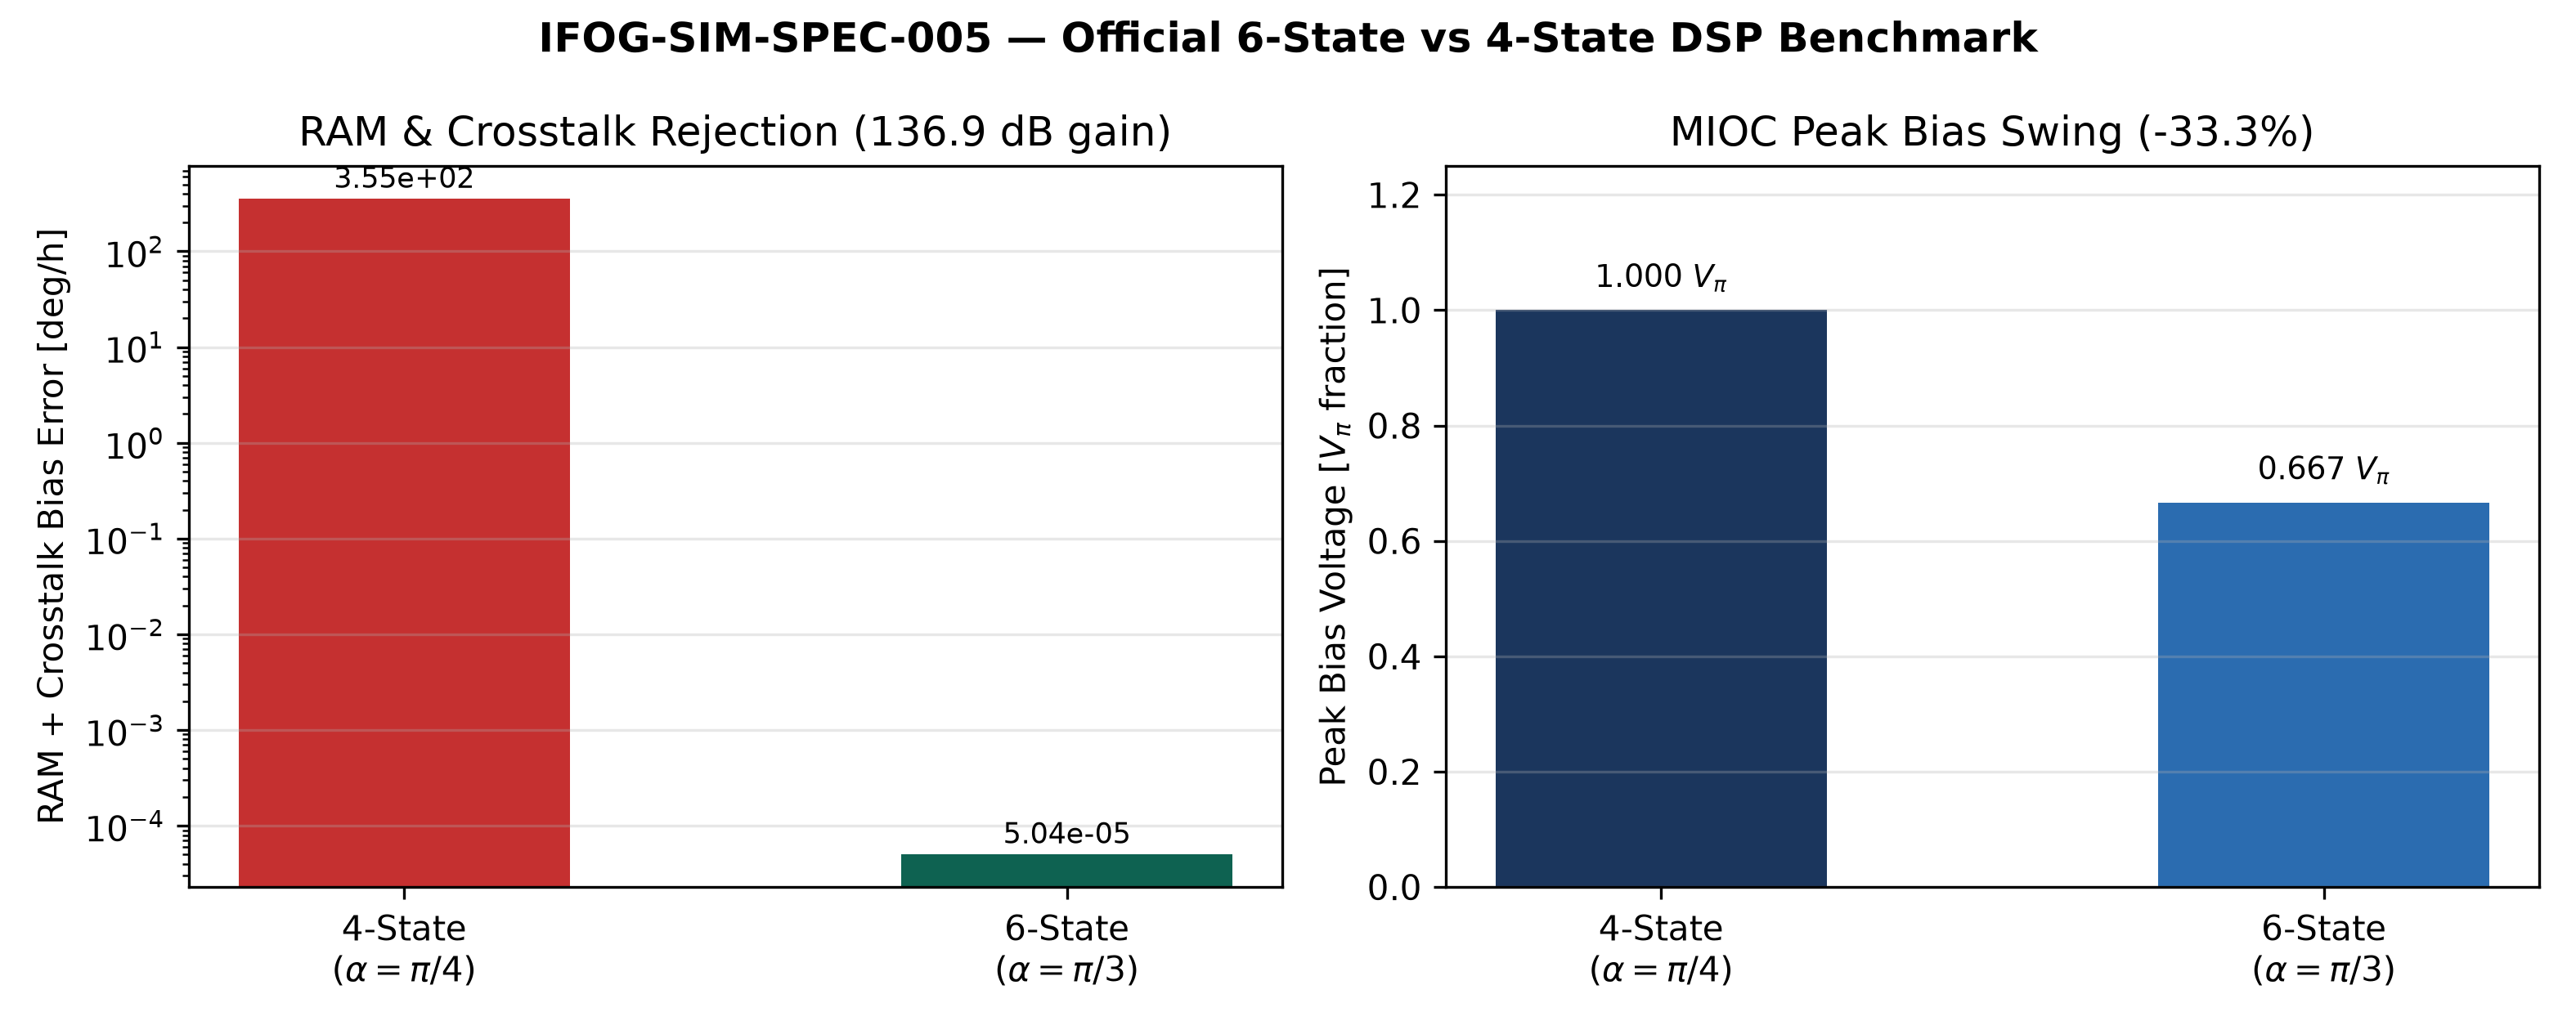
\includegraphics[width=0.90\textwidth,height=0.44\textheight,keepaspectratio]{../examples/full_all_scenarios/figures/dsp6_compare.png}
\end{center}
\vspace{0.02cm}
\begin{columns}[T]
  \begin{column}{0.51\textwidth}
    \begin{eqbox}[Cách đọc 2 Biểu đồ Cột \& Bản chất Vật lý]
      \begin{itemize}\setlength\itemsep{1.6pt}
        \item \textbf{Cột trái (trục Y logarit [$^\circ/\text{h}$]):} Cùng bơm RAM + xuyên nhiễu PCB + $\gamma_{\text{nl}}$: 4-State (cột đỏ) bị trôi mạnh ($354.6^\circ/\text{h}$) do điện áp lái có trung bình DC $\bar{\psi}\ne 0$; 6-State (cột xanh) triệt tiêu về $5.04{\times}10^{-5}\,^\circ/\text{h}$.
        \item \textbf{Cột phải (Biên độ áp đỉnh MIOC):} 6-State chỉ cần biên độ $0.667\,V_\pi$ so với $1.000\,V_\pi$ của 4-State (trong khi 2-State không có Vòng 2 khóa $V_\pi$).
      \end{itemize}
    \end{eqbox}
  \end{column}
  \begin{column}{0.47\textwidth}
    \begin{remarkbox}[Kết luận Kỹ thuật \& Giá trị Thiết kế]
      \begin{itemize}\setlength\itemsep{1.6pt}
        \item Độ lợi triệt tiêu sai số ký sinh đạt \textbf{$+136.94\text{ dB}$} (hơn $7$ triệu lần) mà không cần tăng chi phí phần cứng quang.
        \item Giảm \textbf{$-33.3\%$} biên độ lái MIOC giúp tăng dư địa tuyến tính DAC, giảm công suất tiêu tán và hạ xuyên nhiễu IMU 3 trục xuống $+51.6\text{ dB}$.
      \end{itemize}
    \end{remarkbox}
  \end{column}
\end{columns}
\end{frame}

% SLIDE 26: THỰC NGHIỆM (9/11) — GATE 6: FMI 3.0 BLACK-BOX FMU
\begin{frame}{Kết quả Thực nghiệm (9/11): Kiểm chứng Đóng gói Hộp đen FMI 3.0 FMU}{Gate 6 (\texttt{fmi\_fmu\_gate.png}) \enspace|\enspace Chạy \texttt{build/ifog\_core.fmu} qua \texttt{FMPy} (\texttt{EQ-42..EQ-44})}
\begin{center}
  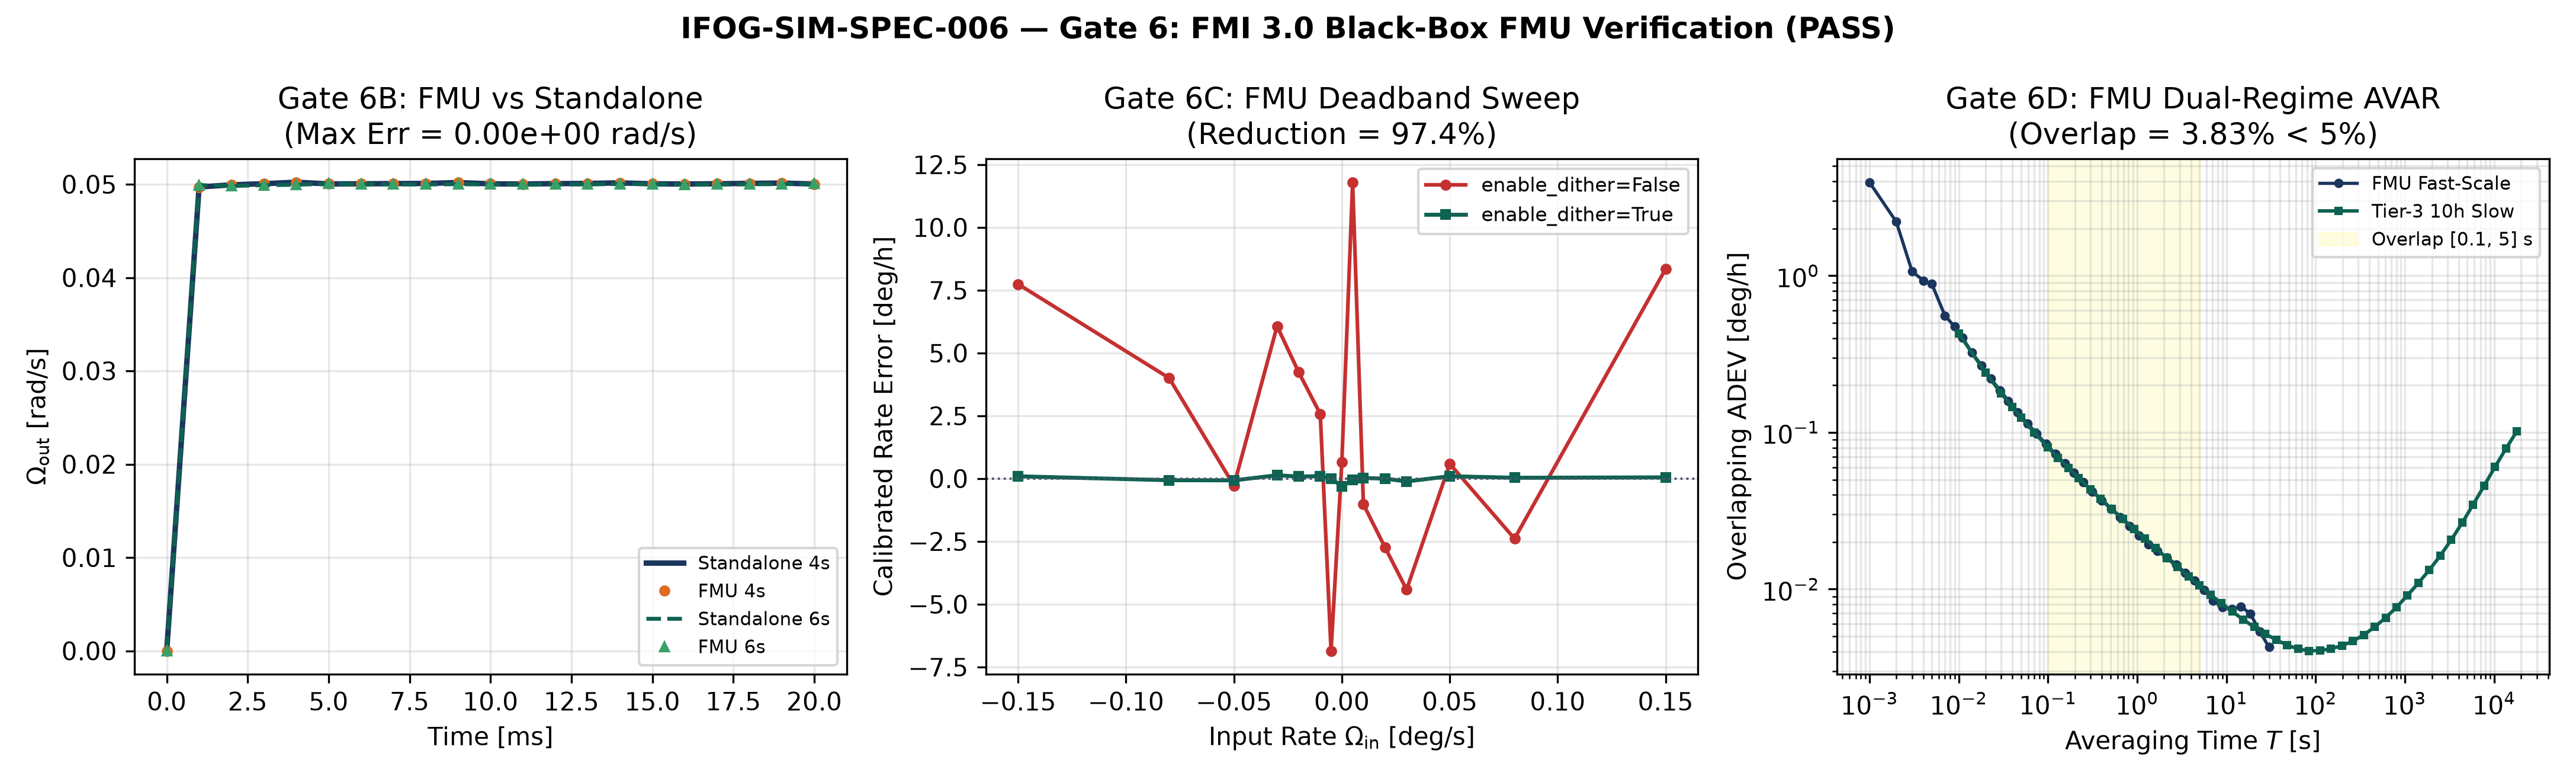
\includegraphics[width=0.95\textwidth,height=0.41\textheight,keepaspectratio]{../examples/full_all_scenarios/figures/fmi_fmu_gate.png}
\end{center}
\vspace{0.02cm}
\begin{columns}[T]
  \begin{column}{0.53\textwidth}
    \begin{eqbox}[Cách đọc 3 Hình Kiểm chứng Hộp đen FMU]
      \begin{itemize}\setlength\itemsep{1.5pt}
        \item \textbf{Hình trái (Đáp ứng bước FMU vs Standalone):} Các điểm rời rạc của \texttt{ifog\_core.fmu} nằm chồng khít 100\% lên đường liên tục của lõi C++ \texttt{ifog\_sim} trên cả 4-State và 6-State.
        \item \textbf{Hình giữa (Quét Deadband qua FMU):} Đường đỏ (tắt dither) hiện gai Deadband; đường xanh (bật dither) phẳng sát $0$.
        \item \textbf{Hình phải (AVAR 5 vùng từ FMU):} Ghép trực tiếp dữ liệu bước $H=1\text{ ms}$ từ FMU sang Tầng 3 10 giờ.
      \end{itemize}
    \end{eqbox}
  \end{column}
  \begin{column}{0.45\textwidth}
    \begin{remarkbox}[Kết luận Nghiệm thu Gate 6]
      \begin{itemize}\setlength\itemsep{1.5pt}
        \item Xác thực lược đồ XML XSD 3.0.2: \textbf{0 lỗi}.
        \item Sai lệch tương đương tối đa: \textbf{\texttt{0.00e+00 rad/s}} (tuyệt đối tới bit cuối cùng).
        \item Giảm Deadband qua FMU: \textbf{97.42\%}; sai lệch vùng chồng AVAR: \textbf{3.83\%} ($<5\%$) — sẵn sàng nhúng vào Simulink/GNC 6-DOF.
      \end{itemize}
    \end{remarkbox}
  \end{column}
\end{columns}
\end{frame}

% SLIDE 27: THỰC NGHIỆM (10/11) — PHY-01: VẬT LÝ DỰ BÁO SPEC-007
\begin{frame}{Kết quả Thực nghiệm (10/11): Kiểm chứng Vật lý Dự báo \texttt{SPEC-007} (\texttt{PHY-01})}{Group D (\texttt{fig\_spec007\_physics\_winding\_mioc.png}) \enspace|\enspace Quấn Octupole, LUT v2 \& Gai MIOC + $C_{\text{xtalk}}$}
\begin{center}
  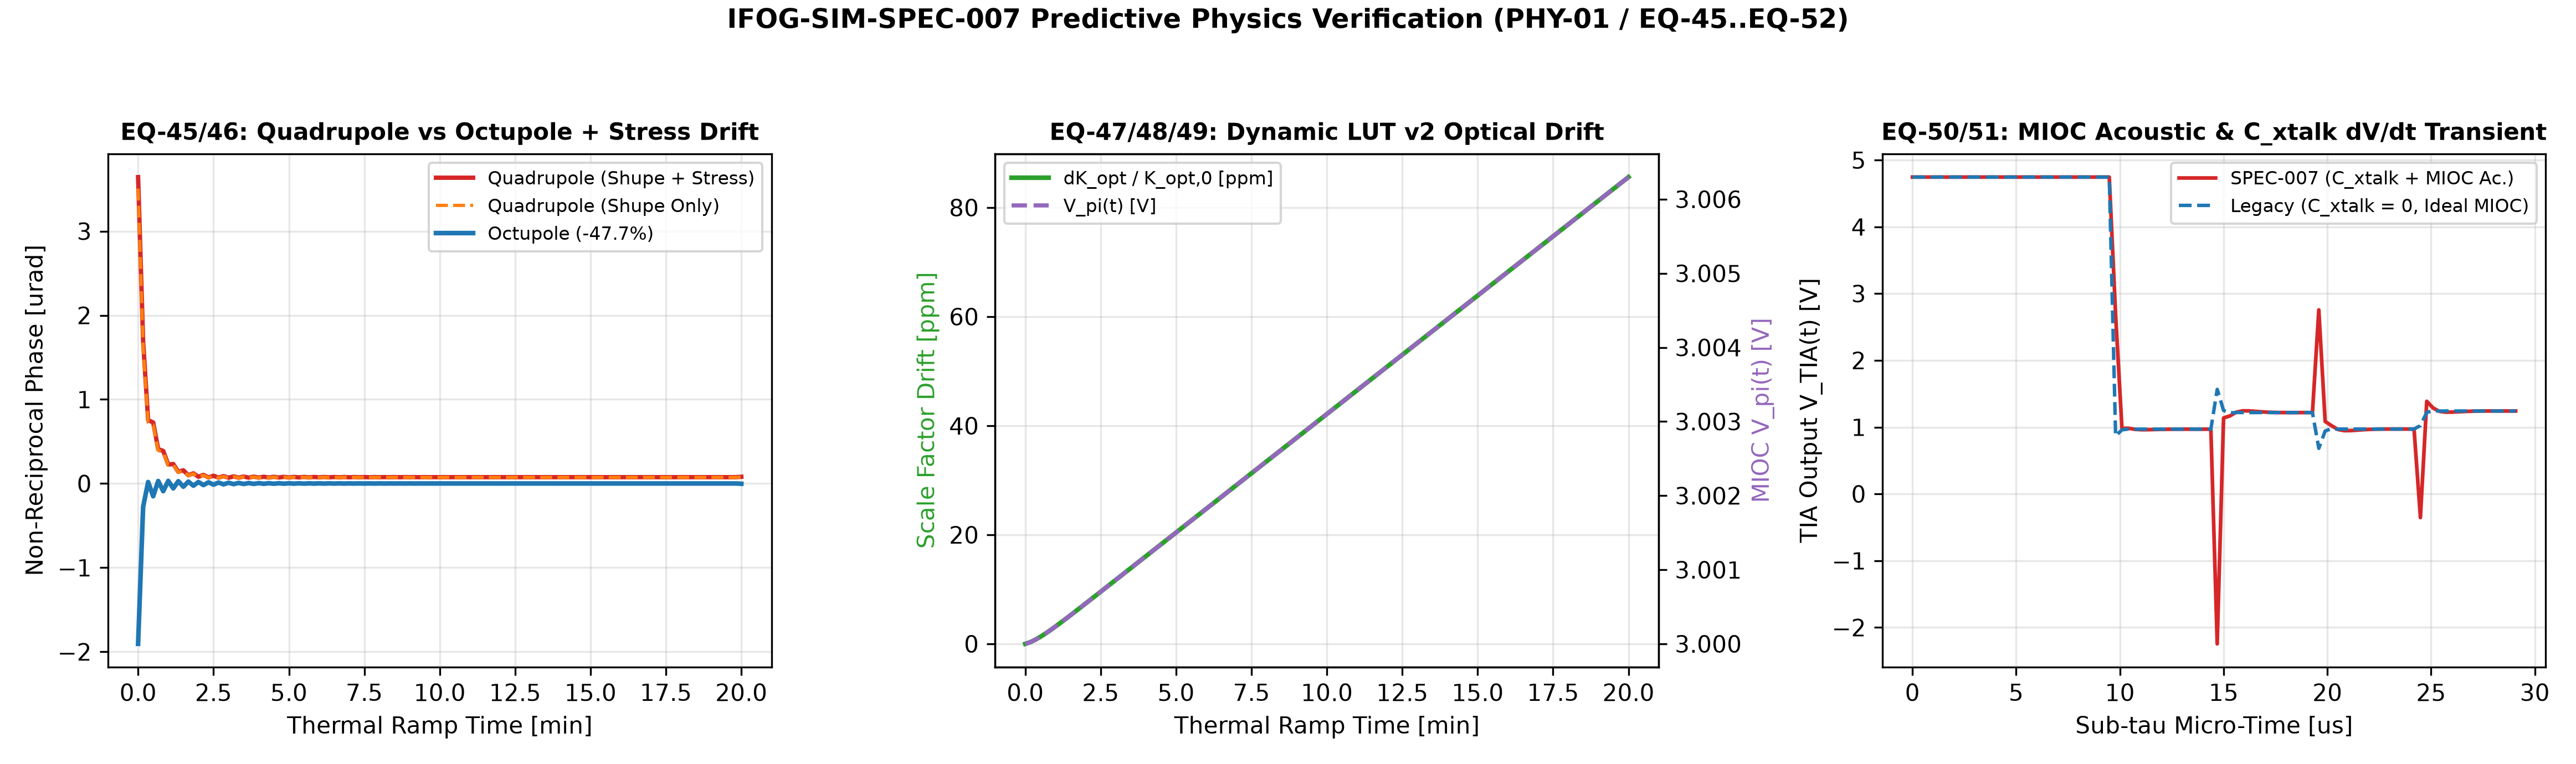
\includegraphics[width=0.95\textwidth,height=0.40\textheight,keepaspectratio]{../examples/full_all_scenarios/figures/fig_spec007_physics_winding_mioc.png}
\end{center}
\vspace{0.02cm}
\begin{columns}[T]
  \begin{column}{0.53\textwidth}
    \begin{eqbox}[Cách đọc 3 Hiện tượng Vật lý Mới trên Hình]
      \begin{itemize}\setlength\itemsep{1.5pt}
        \item \textbf{Hình trái (Pha trôi nhiệt theo thời gian):} Đường đỏ (Quadrupole + Ứng suất) có đỉnh trôi lớn hơn rõ rệt so với đường xanh dương (Octupole 8 lớp) khi buồng nhiệt tăng tốc.
        \item \textbf{Hình giữa (LUT v2 động):} Hai trục tung biểu diễn đồng thời trôi hệ số tỷ lệ $\delta K_{\text{opt}}(t)$ [ppm] và điện áp $V_\pi(t)$ [V] tăng tuyến tính theo nhiệt độ.
        \item \textbf{Hình phải (Zoom sub-$\tau$):} Đường đỏ (có MIOC bậc 2 + $C_{\text{xtalk}}\dot{V}$) bật gai xung nhọn hơn hẳn đường xanh nét đứt (mô hình lý tưởng cũ).
      \end{itemize}
    \end{eqbox}
  \end{column}
  \begin{column}{0.45\textwidth}
    \begin{remarkbox}[Kết luận Kỹ thuật \texttt{PHY-01} (\texttt{EQ-45..52})]
      \begin{itemize}\setlength\itemsep{1.5pt}
        \item Quấn \textbf{Octupole giảm 47.69\%} đỉnh trôi nhiệt Shupe so với Quadrupole.
        \item Bảng \texttt{shupe\_lut.bin} v2 khôi phục chính xác 6 kênh động (sai số \texttt{0.0}, $\delta K_{\text{opt}}=85.59\text{ ppm}$).
        \item Gai xuyên nhiễu điện dung + cộng hưởng MIOC đạt $\Delta V_{\text{TIA}}=\mathbf{0.583\text{ V}}$ — yếu tố then chốt để dự báo chính xác Deadband/Bunny Ears phần cứng.
      \end{itemize}
    \end{remarkbox}
  \end{column}
\end{columns}
\end{frame}

% SLIDE 28: THỰC NGHIỆM (11/11) — CAL-01: HIỆU CHUẨN NGƯỢC (< 5% -> < 1%)
\begin{frame}{Kết quả Thực nghiệm (11/11): Kiểm chứng Hiệu chuẩn Ngược \texttt{CAL-01} ($>40\% \to <1\%$)}{Khớp đồng thời 3 miền thí nghiệm (Static AVAR, Deadband Ramp, Thermal Chamber) đạt chuẩn $<5\%$}
\begin{center}
  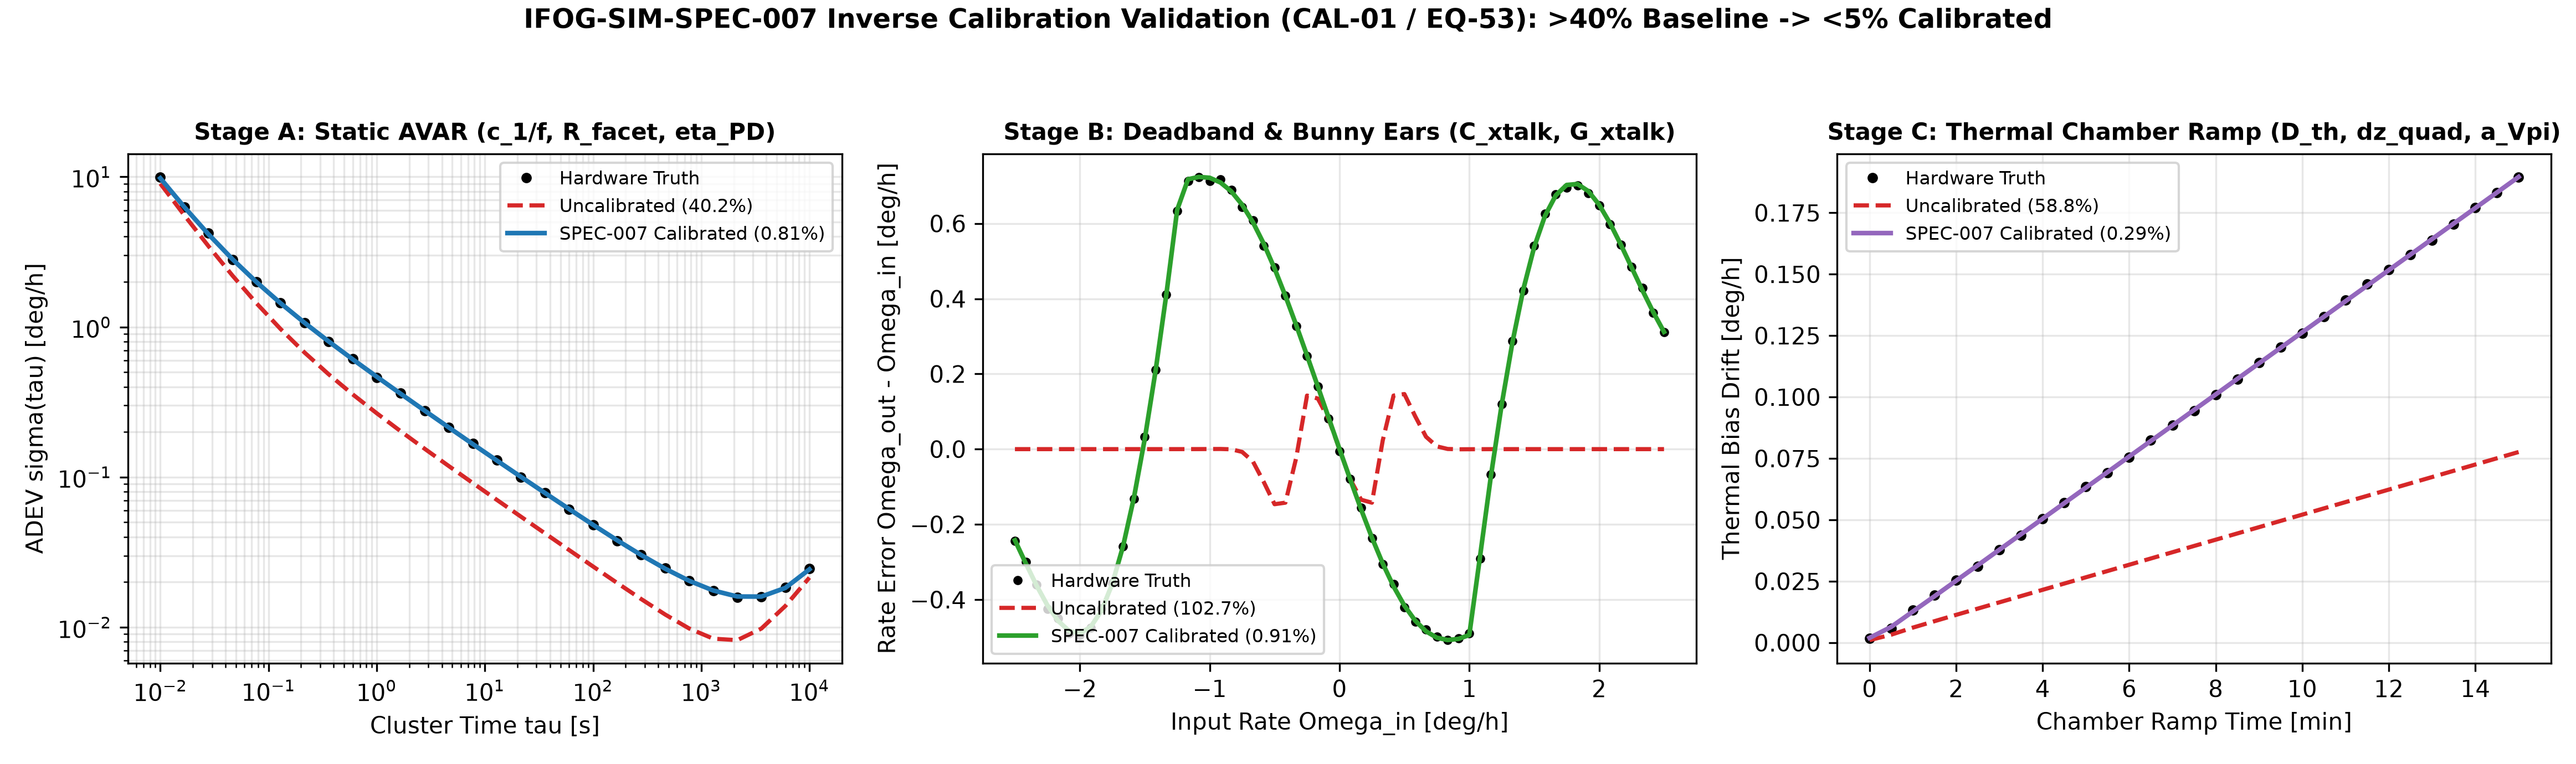
\includegraphics[width=0.95\textwidth,height=0.36\textheight,keepaspectratio]{../examples/full_all_scenarios/figures/fig_spec007_calibration_validation.png}
\end{center}
\vspace{0.01cm}
\begin{columns}[T]
  \begin{column}{0.46\textwidth}
    \begin{remarkbox}[Cách đọc 3 Hình \& Bảng Sai số Trước / Sau HC]
      {\tiny Chấm đen: mẫu thật; đường đỏ đứt: datasheet chưa HC ($>40\%$); đường liền nét: sau \texttt{InverseCalibrator} khớp sát mẫu thật.}
      \vspace{1.5pt}
      \tiny\renewcommand{\arraystretch}{1.04}
      \begin{tabularx}{\linewidth}{@{}X r r c@{}}
        \toprule
        \textbf{Miền đối chiếu} & \textbf{Chưa HC} & \textbf{Sau HC} & \textbf{Ngưỡng} \\
        \midrule
        Static AVAR (5 vùng) & $40.23\%$ & \textbf{0.81\%} & $<5\%$ \\
        Deadband / Bunny Ears & $102.68\%$ & \textbf{0.91\%} & $<5\%$ \\
        Thermal Bias Drift & $58.78\%$ & \textbf{0.29\%} & $<5\%$ \\
        Scale Factor Drift & $52.30\%$ & \textbf{0.04\%} & $<5\%$ \\
        \bottomrule
      \end{tabularx}
    \end{remarkbox}
  \end{column}
  \begin{column}{0.52\textwidth}
    \begin{eqbox}[Ý nghĩa \& Kiểm chứng Chéo trên Lõi C++ Thật]
      \begin{itemize}\setlength\itemsep{1.8pt}
        \item \textbf{Ý nghĩa hình vẽ:} Chứng minh khi chỉ dùng thông số datasheet (đường đỏ), mô hình bỏ sót hoàn toàn biên độ Bunny Ears và trôi nhiệt thực tế; sau 3 giai đoạn TRF, đường mô phỏng trùng khít thực nghiệm trên cả 3 miền.
        \item \textbf{Hồi phục tham số ẩn:} Cả \textbf{10 / 10 tham số ký sinh} phục hồi trong sai số \textbf{$\le 2.18\%$}.
        \item \textbf{Kiểm chứng chéo C++ Tầng 2:} Sai số dự báo tốc độ góc vòng kín đạt \textbf{0.034\%}, xuất sẵn \texttt{calibrated\_params.json} kèm 95\% CI.
      \end{itemize}
    \end{eqbox}
  \end{column}
\end{columns}
\end{frame}

% SLIDE 29: MA TRẬN 23 KỊCH BẢN & TRIỂN KHAI TÁI LẬP
\begin{frame}{Hệ thống 23 Kịch bản Chuẩn hóa, CLI \& Khả năng Tái lập Thực nghiệm}{Chạy độc lập từng bài toán vật lý hoặc toàn bộ 23/23 kịch bản trên Linux / Docker}
\scriptsize
\renewcommand{\arraystretch}{1.08}
\begin{tabularx}{\textwidth}{@{}p{2.3cm} p{2.7cm} >{\raggedright\arraybackslash}X c@{}}
\toprule
\textbf{Nhóm Kịch bản} & \textbf{Lệnh CLI (\texttt{--mode})} & \textbf{Nội dung kiểm chứng khoa học chính} & \textbf{Kết quả} \\
\midrule
\textbf{Core Gates 1--4} & \texttt{full} (\texttt{gate1..4}) & Tuyến tính $2\pi$ flyback, Deadband/Bunny Ears, $1/f$ \& $\mathbf{K}$, AVAR 5 vùng 10h & \textcolor{AcadTeal}{\textbf{4/4 PASS}} \\
\textbf{Gate 5 (6-State)} & \texttt{dsp6\_compare} & 6-State đối xứng ($\alpha^*=\pi/3$): $-33.3\%$ áp đỉnh, $+136.9\text{ dB}$ khử RAM/xtalk & \textcolor{AcadTeal}{\textbf{PASS}} \\
\textbf{Gate 6 (FMI 3.0)} & \texttt{fmi\_gate} & XSD 0 lỗi, tương đương \texttt{0.00e+00 rad/s}, Deadband 97.4\%, AVAR 3.83\% & \textcolor{AcadTeal}{\textbf{PASS}} \\
\textbf{Group A (TD)} & \texttt{td\_all} (\texttt{TD-01..06}) & Blanking $k^*=5$, Bode 2.54 kHz, sốc $V_\pi$, $700^\circ/\text{s}$ anti-windup, Shupe, PRBS & \textcolor{AcadTeal}{\textbf{6/6 PASS}} \\
\textbf{Group B (ENG)} & \texttt{eng\_all} (\texttt{ENG-01..05}) & BOM ENOB/Jitter, IMU 3 trục ($+51.6\text{ dB}$), VRE/Mu-metal, 5 lỗi BIT, MC $N=500$ & \textcolor{AcadTeal}{\textbf{5/5 PASS}} \\
\textbf{Group C (DYN)} & \texttt{dyn\_all} (\texttt{DYN-01..04}) & Đáp ứng bước, Bode Mag/Phase/GD 15 điểm, Output PSD, Sine soi PD/$V_{\text{fb}}$ & \textcolor{AcadTeal}{\textbf{4/4 PASS}} \\
\textbf{Group D (SPEC-007)} & \texttt{spec007\_all} (\texttt{PHY/CAL}) & Quấn Octupole ($-47.7\%$), LUT v2, MIOC+$C_{\text{xtalk}}$ \& Hiệu chuẩn ngược $<1\%$ & \textcolor{AcadTeal}{\textbf{2/2 PASS}} \\
\bottomrule
\end{tabularx}

\vspace{0.18cm}
\begin{columns}[T]
  \begin{column}{0.49\textwidth}
    \begin{eqbox}[Tái lập trực tiếp trên Linux (Native Build)]
      \texttt{bash scripts/setup\_env.sh --build-tier2 --verify}\\
      \texttt{source scripts/env.sh}\\
      \texttt{./scripts/run\_sim.sh --mode spec007\_all}\\
      \texttt{./scripts/run\_all\_scenarios.sh --mc-runs 500}
    \end{eqbox}
  \end{column}
  \begin{column}{0.49\textwidth}
    \begin{remarkbox}[Tái lập tức thì qua Container (Docker / Podman)]
      \texttt{./scripts/container\_run.sh build}\\
      \texttt{./scripts/container\_run.sh sim --mode fmi\_gate}\\
      \texttt{./scripts/container\_run.sh example}\\
      {\scriptsize Tự động sinh \texttt{report/<id>/\{report.md, report.html, figures/*.png\}}.}
    \end{remarkbox}
  \end{column}
\end{columns}
\end{frame}

% SLIDE 30: CHẤT LƯỢNG, CI/CD DIFF FILTER & TÀI LIỆU THAM KHẢO
\begin{frame}{Đảm bảo Chất lượng, CI/CD Chọn lọc theo Diff \& Tài liệu Tham khảo}{Tổng kết kỹ thuật \texttt{ifog-vproto \DocVersion} và cơ sở học thuật}
\begin{columns}[T]
  \begin{column}{0.50\textwidth}
    \begin{eqbox}[1. Kiểm chứng Chất lượng \& CI/CD Thông minh]
      \begin{itemize}\setlength\itemsep{2.8pt}
        \item \textbf{Độ phủ mã nguồn kép 100.0\%:}
          \begin{itemize}\setlength\itemsep{1pt}
            \item C++ (\texttt{tier2\_sysc\_ams/} + \texttt{fmi\_wrapper/src/}): \textbf{2,329 / 2,329 dòng} (\textbf{100.0\%}, 211/211 hàm qua \texttt{gcovr}).
            \item Python (\texttt{tier1}, \texttt{tier3}, \texttt{viz}): \textbf{100.00\%} dòng (\texttt{pytest-cov}, 4,770/4,770 stmts).
          \end{itemize}
        \item \textbf{Truy vết công thức 1-đối-1:} Toàn bộ \textbf{53 / 53 công thức} (\texttt{EQ-01..53}) có bài kiểm thử tự động trong CI.
        \item \textbf{Khóa toàn vẹn Đặc tả (Rule 7) \& Đồng bộ (Rule 16):} Xác thực SHA-256 cho \texttt{SPEC-004..007} và tài liệu phát hành.
        \item \textbf{Bộ lọc Diff CI/CD (\texttt{scripts/ci\_diff\_filter.py}):} Tự phân tích \texttt{git diff} tại bước \texttt{detect-changes} — \textbf{chỉ kích hoạt CI/CD khi mã nguồn/cấu hình/đặc tả thay đổi}, tự bỏ qua khi chỉ sửa tài liệu (\texttt{docs/}, slide, \texttt{README.md}).
      \end{itemize}
    \end{eqbox}
  \end{column}
  \begin{column}{0.48\textwidth}
    \begin{remarkbox}[2. Tài liệu Tham khảo \& Chuẩn mực Khoa học]
      \scriptsize
      \begin{enumerate}\setlength\itemsep{1.8pt}
        \item \textbf{IEEE Std 952-2020}, \emph{Specification Format Guide and Test Procedure for Single-Axis Interferometric Fiber Optic Gyros}.
        \item H. C. Lefèvre, \emph{The Fiber-Optic Gyroscope}, 3rd Ed., Artech House, 2022.
        \item M. Barnasconi \emph{et al.}, \emph{SystemC AMS Extensions User's Guide} (TDF \& LTF \texttt{sca\_ltf\_nd}), Accellera Systems Initiative / \textbf{IEEE Std 1666.1-2016}.
        \item D. M. Shupe, ``Thermally induced nonreciprocity in the fiber-optic interferometer,'' \emph{Applied Optics}, 19(5):654--655, 1980.
        \item F. Mohr, ``Thermooptically induced bias drift in fiber optical Sagnac interferometers,'' \emph{J. Lightwave Technol.}, 14(1):27--41, 1996.
        \item \textbf{Modelica Association}, \emph{Functional Mock-up Interface (FMI) Specification 3.0.2}, 2024.
      \end{enumerate}
    \end{remarkbox}
  \end{column}
\end{columns}
\end{frame}

\end{document}
